\chapter{Electronic excitations}\label{chap:10}
An electron--hole pair is the signal most searches for sub-GeV dark matter look for. A single pair in silicon costs at least the gap, \SI{1.17}{eV}, and a pair is easy to count: the charge-coupled devices of \cref{sec:1.5} read out one electron at a time. Dark matter of \SI{1}{MeV} carries at most \SI{3.5}{eV} of kinetic energy, enough to cross the gap, and this is why electron scattering in semiconductors reaches masses that nuclear recoils cannot. \Cref{chap:8} wrote the rate for any coupling as a contraction of the response matrix with a tensor from the dark-matter side, and \cref{chap:9} placed each electronic excitation on the map of channels. How faithfully can the rate of making pairs be computed in a real crystal? The band structure alone gives the crystal form factor. The answer depends on what the band structure leaves out: other electrons that screen the potential and bind the pair, couplings to spin and current rather than number, and particles that are absorbed, split or fast rather than slow and elastic. Throughout, the nuclei stay clamped. This is the electronic sector of \cref{sec:8.6}, and the lattice enters only in \crefrange{chap:11}{chap:13}, while the pairs made here are followed into the detector in \cref{chap:18}. We start from independent electrons and add, one at a time, the pieces of the response that they leave out (\cref{fig:10-map}).

\begin{figure}[tbp]
  \centering
  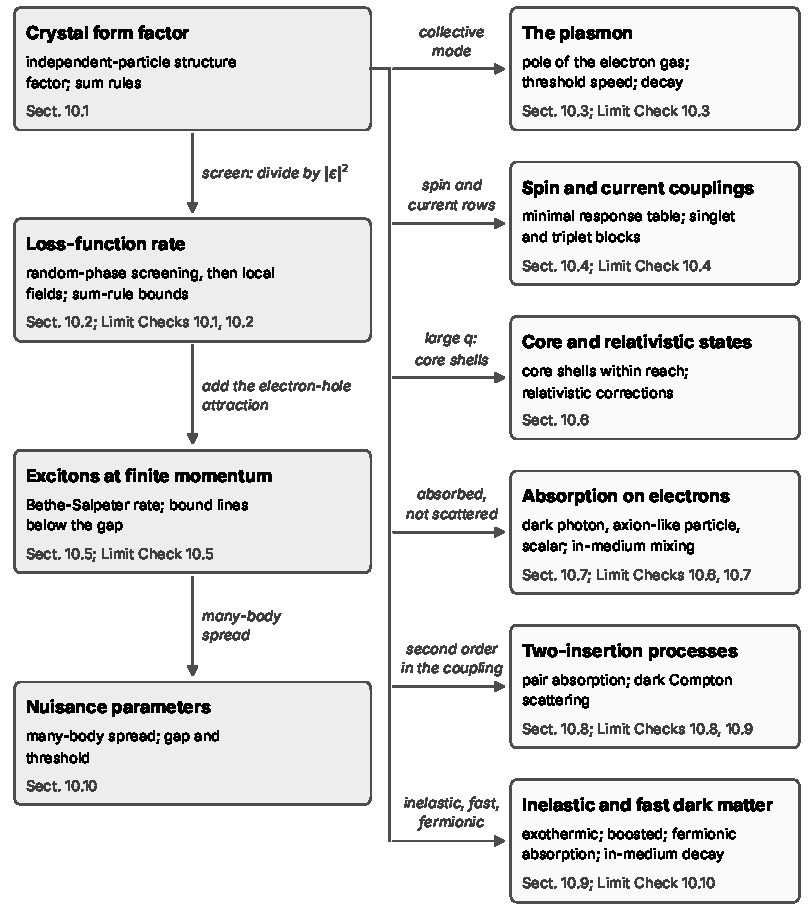
\includegraphics[width=0.85\linewidth]{figures/ch10/map10.pdf}
  \caption{The electronic response and its extensions. Left, the hierarchy of approximations to the density response: the independent-particle crystal form factor (\cref{sec:10.1}), screened by $|\varepsilon|^2$ in the random-phase approximation and then with local fields (\cref{sec:10.2}; \cref{lim:10.2a,lim:10.2b}), with the electron--hole attraction added (\cref{sec:10.5}; \cref{lim:10.5a}); the step to the next approximation is the theory uncertainty of the rate, collected in its uncertainty budget (\cref{sec:10.10}). Right, the response classes beyond slow, elastic scattering on the density: the plasmon (\cref{sec:10.3}; \cref{lim:10.3b}), spin and current rows (\cref{sec:10.4}; \cref{lim:10.4a}), core shells at large $q$ (\cref{sec:10.6}), absorption (\cref{sec:10.7}; \cref{lim:10.7a,lim:10.7b}), processes second order in the coupling (\cref{sec:10.8}; \cref{lim:10.8a}), and inelastic, boosted or fermionic dark matter (\cref{sec:10.9}; \cref{lim:10.9d}).}
  \label{fig:10-map}
\end{figure}

\section{The crystal form factor}\label{sec:10.1}

A dark-matter particle of \SI{10}{MeV} that crosses silicon can transfer up to \SI{53}{keV} of momentum and deposit up to \SI{35}{eV} (\cref{tab:1-kinematics}). Whether it leaves an electron--hole pair behind depends, for each pair $(\vect{q},\omega)$, on how strongly the filled bands respond at that momentum and energy. In the simplest description of the crystal, electrons that move independently in the potential of clamped nuclei, that response is a sum over transitions from one valence state to one conduction state, each weighted by the square of the density vertex of \cref{sec:3.2}. Experiments quote it as the \emph{crystal form factor} of Essig and collaborators~\cite{essig2016direct}, and nearly every projected or published limit on electron scattering in silicon and germanium rests on a table of it.

\subsection{The independent-particle structure factor}

Electron scattering through a mediator that couples to the electron number uses one row of the master formula, the density $n_e(\vect{q})$, with $\mathfrak{D}_{ee} = |\tilde V(\vect{q})|^2$ and all other entries zero (\cref{sec:8.2}). The spectrum per unit target mass is then \cref{eq:8.2-spectrum} with the dynamic structure factor of the electrons in place of the contraction, which is \cref{eq:A.8-rate}.

At the base point $\mathfrak{T}_0$ of the expansion hierarchy, \cref{eq:8.5-base}, the nuclei are clamped, the temperature is zero and the electrons are independent particles. The ground state is then a single Slater determinant $|0\rangle$ in which the four valence bands of silicon are filled with both spins and the conduction bands are empty. The one-electron states are Kohn--Sham states, and the conduction energies are raised by the scissor shift of \cref{sec:3.4}, which leaves the states themselves unchanged.

In the Bloch basis the density operator is \cref{eq:3.2-ne}. Acting on $|0\rangle$, a term $c^\dagger_{m,\vect{k}+\vect{q},s}c_{n\vect{k}s}$ vanishes if $n$ is a conduction band, since there is no electron to remove, and if $m$ is a valence band, since the state is already occupied, unless it is the state just emptied. That exception requires $\vect{k} + \vect{q} \equiv \vect{k}$, that is $\vect{q} = \vect{G}$, and it returns $|0\rangle$ itself with $\omega = 0$, the elastic Bragg term that no detector sees. For $\omega > 0$,
\begin{equation}
  n_e(\vect{q})|0\rangle = \sum_s\sum_{\vect{k}\in\mathrm{BZ}}\sum_{v,c}\rho_{cv}(\vect{k},\vect{q})\,|c,\vect{k}+\vect{q},s;\,v\vect{k}s\rangle ,
  \label{eq:D.29-pairs}
\end{equation}
where the ket is $|0\rangle$ with the electron moved from $v\vect{k}s$ to $c,\vect{k}+\vect{q},s$. These pair states are orthonormal, and their energies above the ground state are $\varepsilon_{c,\vect{k}+\vect{q}} - \varepsilon_{v\vect{k}}$, with $\vect{k} + \vect{q}$ folded into the first zone by the Umklapp vector $\vect{G}_{\mathrm{U}}$ of \cref{eq:3.2-rho}. Each pair appears once in \cref{eq:D.29-pairs}: at fixed $\vect{q}$ the hole $v\vect{k}s$ fixes the crystal momentum of the electron. Inserting \cref{eq:D.29-pairs} into \cref{eq:4.2-Sab} with $a = b = n_e$, the two spins give equal terms, and the sum over the $N$ crystal momenta of the zone becomes $\Vol\int_{\mathrm{BZ}}\dd^3k/(2\pi)^3$ with $\Vol = N\Omega$ (\cref{sec:3.1}). The volume cancels against the $1/\Vol$ in the definition of $S$, and
\begin{keyresult}[Independent-particle structure factor of a semiconductor]
\begin{equation}
  S^0(\vect{q},\omega) = 4\pi\sum_{v,c}\int_{\mathrm{BZ}}\frac{\dd^3k}{(2\pi)^3}\,\bigl|\rho_{cv}(\vect{k},\vect{q})\bigr|^2\,\delta\bigl(\omega - \varepsilon_{c,\vect{k}+\vect{q}} + \varepsilon_{v\vect{k}}\bigr) ,
  \label{eq:10.1-S0}
\end{equation}
for $\omega > 0$ at $T = 0$, with $v$ over the valence and $c$ over the conduction bands. The electron-recoil rate at $\mathfrak{T}_0$ is \cref{eq:8.2-spectrum} with $\mathfrak{D}_{ee} = \pi\sigmae\FDM(q)^2/\mu_{\chi e}^2$ (\cref{eq:1.4-Vsq}) and $S = S^0$.
\end{keyresult}
\noindent The factor $4\pi$ in $S^0$ is the $2\pi$ of \cref{eq:4.2-Sab} times 2 for spin. Each transition counts once, with the square of an amplitude of order one, and the rate is a sum of $|\rho_{cv}|^2$ over pairs, weighted by energy conservation. The same expression is $-2\Imag R^0_{\vect{0}\vect{0}}(\vect{q},\omega)$, the head of the independent-particle bubble \cref{eq:4.6-R0} at $T = 0$: in the bubble, a pair costs $\varepsilon_{c,\vect{k}+\vect{q}} - \varepsilon_{v\vect{k}}$ and its resonant denominator carries the imaginary part $-\pi\delta(\omega - \varepsilon_{c,\vect{k}+\vect{q}} + \varepsilon_{v\vect{k}})$. So the codes that compute dielectric functions compute $S^0$ along the way, and the screened response of \cref{sec:10.2} starts from the same object.

As in \cref{chap:3}, $S^0$ vanishes below the smallest pair energy $E_{\mathrm{min}}(\vect{q})$ of \cref{eq:3.3-Emin}, and a mass is kinematically allowed only where \cref{eq:3.3-allowed} holds. Its total weight is fixed by the closure relation \cref{eq:3.2-closure}, each valence state distributes a total weight of one over all bands at $\vect{k}+\vect{q}$, and only the part that lands in conduction bands counts. The zeroth moment is therefore at most $4\pi\cdot4/\Omega$, four valence bands of unit weight, a bound reached only when every transition leads into a conduction band. At small $q$ most of the weight stays in the same band and is lost to the rate; at large $q$ it spreads over conduction bands far above the gap.

Its energy-weighted sum is fixed as well. For a local one-electron potential, the double commutator of \cref{sec:4.3} taken for one electron gives $\sum_m(\varepsilon_{m,\vect{k}+\vect{q}} - \varepsilon_{n\vect{k}})|\rho_{mn}(\vect{k},\vect{q})|^2 = q^2/2m_e$ for every state $n\vect{k}$, the sum running over all bands $m$. The terms in which $m$ is another valence band are absent from \cref{eq:10.1-S0}, but summed over $\vect{k}$ they cancel: each transition at $-\vect{q}$ is the reverse of one at $\vect{q}$, so the valence--valence sum at $-\vect{q}$ is minus the sum at $\vect{q}$, while $S^0(\vect{q},\omega) = S^0(-\vect{q},\omega)$ in silicon makes the two sums equal, and a sum equal to its own negative vanishes. The first moment of \cref{eq:10.1-S0} is then $4\pi\cdot4\cdot\Omega^{-1}\cdot q^2/2m_e = \pi\nd_eq^2/m_e$ with $\nd_e = 8/\Omega$, the $f$-sum rule \cref{eq:4.3-fsum} for the valence electrons, since $\int_{\mathrm{BZ}}\dd^3k/(2\pi)^3 = 1/\Omega$. It is the standard test of a computed $S^0$, with the caveats of \cref{sec:4.3} for nonlocal potentials.

Note that $\vect{q}$ in \cref{eq:10.1-S0} is the physical momentum transfer and is never folded. The crystal momentum of the final electron is $\vect{k} + \vect{q}$ reduced to the first zone, but the vertex $\rho_{cv}$ depends on the whole $\vect{q}$ through the Umklapp vector that stays in the plane wave (\cref{eq:3.2-rho}), and so do $\vmin$ and $\FDM$ on the dark-matter side (\cref{sec:1.3}). Two momentum transfers that differ by a reciprocal-lattice vector reach the same pairs with different amplitudes and different kinematic weights.

The structure factor of a crystal depends on the direction of $\vect{q}$, and the full velocity kernel of \cref{eq:8.2-spectrum} gives a rate that changes as the Earth turns the crystal through the dark-matter wind, the daily modulation of \cref{sec:11.7}. For the time-averaged rate of a target whose orientation is not resolved, the literature replaces $S^0$ by its average $\bar S^0(q,\omega)$ over the directions of $\vect{q}$. The velocity and angular integrals then reduce to the mean inverse speed, \cref{eq:A.8-eta}. The rate takes the isotropic form \cref{eq:A.8-rateiso},
\begin{equation}
  \frac{\dd\mathcal{R}}{\dd\omega} = \frac{\rho_\chi\,\sigmae}{4\pi\,\mchi\,\rho_T\,\mu_{\chi e}^2}\int q\,\dd q\;\FDM(q)^2\,\eta\bigl(\vmin(q,\omega)\bigr)\,\bar S^0(q,\omega) .
  \label{eq:10.1-rateiso}
\end{equation}
\Cref{app:A.8} explains why this is not the same as averaging the directional rate over a day: a detector at fixed latitude does not sample all orientations equally.

\subsection{Form-factor normalizations}

Essig, Fernandez-Serra, Mardon, Soto, Volansky and Yu wrote the same rate per target, with the target information collected into a dimensionless function~\cite[Eqs.~(3.13) and (3.17)]{essig2016direct}. In our notation their crystal form factor is
\begin{equation}
  |f_{\mathrm{crys}}(q,\omega)|^2 = \frac{q^3\,\Omega}{4\pi\alpha\,m_e^2}\,\bar S^0(q,\omega) ,
  \label{eq:10.1-fcrys}
\end{equation}
which is \cref{eq:A.8-fcrys} at $\mathfrak{T}_0$. The factor $q^3/\alpha m_e^2$ is chosen so that $|f_{\mathrm{crys}}|^2$ is close to one where the rate is made. We substitute $\Omega\bar S^0 = 4\pi\alpha m_e^2|f_{\mathrm{crys}}|^2/q^3$ into \cref{eq:10.1-rateiso} and use $\rho_T\Omega = M_{\mathrm{cell}}$, the cell mass:
\begin{equation}
  \begin{aligned}
  \frac{\dd\mathcal{R}}{\dd\omega} &= \frac{\rho_\chi\,\sigmae\,\alpha\,m_e^2}{\mchi\,M_{\mathrm{cell}}\,\mu_{\chi e}^2} \\
  &\quad\times\int\frac{\dd q}{q^2}\,\eta\bigl(\vmin(q,\omega)\bigr)\,\FDM(q)^2\,|f_{\mathrm{crys}}(q,\omega)|^2 .
  \end{aligned}
  \label{eq:D.29-rate}
\end{equation}
Multiplying by $\omega$ turns $\dd q/q^2$ into $\dd\ln q\,(\omega/q)$ and the left side into $\dd\mathcal{R}/\dd\ln\omega$. Of the crystal, only the cell mass is left outside the form factor, because $|f_{\mathrm{crys}}|^2$ is defined per cell:
\begin{limitbox}[Crystal form-factor rate][lim:10.1a]
At independent-particle level, unscreened, at zero temperature and with clamped nuclei, the electron-recoil spectrum per unit target mass is
\begin{equation*}
  \begin{aligned}
  \frac{\dd\mathcal{R}}{\dd\ln\omega} &= \frac{\rho_\chi\,\sigmae\,\alpha\,m_e^2}{\mchi\,M_{\mathrm{cell}}\,\mu_{\chi e}^2} \\
  &\quad\times\int\dd\ln q\;\frac{\omega}{q}\,\eta\bigl(\vmin(q,\omega)\bigr)\,\FDM(q)^2\,|f_{\mathrm{crys}}(q,\omega)|^2 ,
  \end{aligned}
\end{equation*}
after Ref.~\cite[Eqs.~(3.13) and (3.17)]{essig2016direct}, divided by the target mass.
\par\smallskip
{\centering
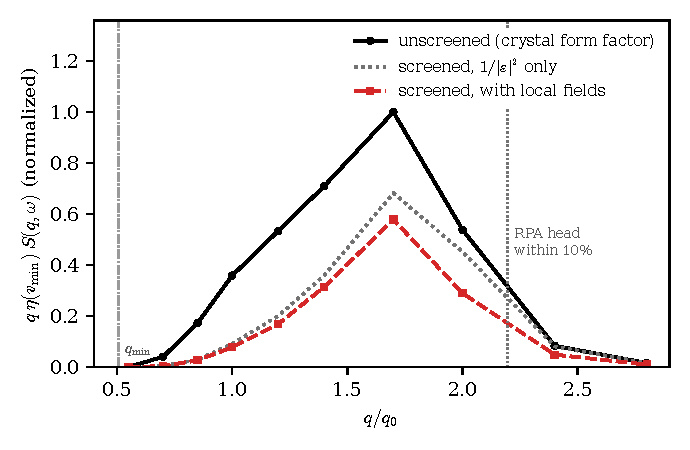
\includegraphics[width=\linewidth]{figures/ch10/limit10_1a.pdf}
\captionof{figure}{Unscreened rate against screened rates in silicon at $\omega = \SI{5}{eV}$, for $\mchi = \SI{10}{MeV}$ and a heavy mediator: the rate weight $q\,\eta(\vmin)\,S(q,\omega)$ of \cref{eq:10.1-rateiso} against $q$, normalized to the maximum of the unscreened curve. All three curves come from one model, the local empirical pseudopotential of \cref{we:8-lf-nuisance} (model gap \SI{0.82}{eV}), with $\vect{q}$ along the direction $(5,3,1)$, chosen so that no $\vect{q} + \vect{G}$ comes close to zero, and spectra averaged over 4.5 to \SI{5.5}{eV}. Solid: independent particles, the crystal form factor of the box. Dotted: random-phase screening by the macroscopic $1/|\varepsilon|^2$ alone, the leading correction. Dashed: random-phase screening with local fields over the 51 shortest reciprocal-lattice vectors, the fuller result. Dash-dotted: the smallest $q$ the halo reaches at \SI{5}{eV}. Dotted vertical: above $2.2\,q_0 = \SI{8.2}{keV}$, with $q_0 = \alpha m_e$, the macroscopic screening changes the rate by less than 10 percent. The model has no momentum components above $2.8\,q_0$, where the plot ends. Nothing is shaded. No $q$ in the plotted range brings the fuller result within 10 percent of the unscreened one.}\label{fig:10-fcrys-limit}
\par}
\smallskip
Near the kinematic edge the unscreened formula overstates the response twentyfold, at $q_0$ fourfold; macroscopic screening fades above about \SI{8}{keV}, but local fields keep the screened response near 0.6 of the unscreened one up to the largest $q$ this model can describe.
\end{limitbox}
\noindent The leading correction to the box lies on the many-body axis $\mathcal{X}$ of \cref{sec:8.5}: the polarization of the valence electrons screens the dark matter's potential and multiplies the response at small $q$ by roughly $1/|\varepsilon(q,\omega)|^2$, and the local fields of the crystal modify that factor. \Cref{sec:10.2} adds both. In silicon at \SI{5}{eV} the correction is not small (\cref{fig:10-fcrys-limit}). The kinematic edge at that energy lies at $0.525\,q_0$, with $q_0 = \alpha m_e = \SI{3.73}{keV}$; just above it, at $q = 0.55\,q_0$, screening cuts the response to 0.05 of the unscreened value, and at $q_0$ to 0.22. The local fields do not fade with $q$ as the macroscopic factor does: between 2 and $2.8\,q_0$ they hold the response at 0.54 to 0.61 of the unscreened value, with an uncertainty of about 10 percent from the size of the set of reciprocal-lattice vectors. Integrated over $q$, the screened rate at \SI{5}{eV} is 0.47 of the unscreened one. The model is cruder than the tabulated form factor, which it matches to within 25 percent at $q_0$, and \cref{sec:10.2} computes the same ratios from first-principles tables.

Written out with \cref{eq:10.1-S0}, $|f_{\mathrm{crys}}|^2$ is a double integral over the initial and final crystal momenta $\vect{k}$ and $\vect{k}'$ and a sum over the Umklapp vectors $\vect{G}'$ that connect them, the form in which Ref.~\cite[Eq.~(3.17)]{essig2016direct} defines it. For any function $g(\vect{q})$,
\begin{equation*}
  \int\frac{\dd^2\hat{\vect{q}}}{4\pi}\,g(q\hat{\vect{q}}) = \frac{1}{4\pi q^2}\int\dd^3q'\,\delta(q - |\vect{q}'|)\,g(\vect{q}') ,
\end{equation*}
since $\dd^3q' = q'^2\dd q'\,\dd^2\hat{\vect{q}}'$. At fixed $\vect{k}$, every $\vect{q}'$ is reached exactly once as $\vect{q}' = \vect{k}' - \vect{k} + \vect{G}'$ with $\vect{k}'$ in the first zone and $\vect{G}'$ a reciprocal-lattice vector, because the zones translated by all $\vect{G}'$ tile space. Then $\int\dd^3q' = \sum_{\vect{G}'}\int_{\mathrm{BZ}}\dd^3k'$, the final crystal momentum is $\vect{k}'$, and $\vect{G}'$ is the Umklapp vector of the transition. Applied to \cref{eq:10.1-S0},
\begin{equation*}
  \begin{aligned}
  \bar S^0(q,\omega) &= \frac{(2\pi)^3}{q^2}\sum_{v,c}\int_{\mathrm{BZ}}\frac{\dd^3k}{(2\pi)^3}\int_{\mathrm{BZ}}\frac{\dd^3k'}{(2\pi)^3}\sum_{\vect{G}'}\delta(q - |\vect{k}' - \vect{k} + \vect{G}'|) \\
  &\quad\times|\rho_{cv}(\vect{k},\vect{k}'-\vect{k}+\vect{G}')|^2\,\delta(\omega - \varepsilon_{c\vect{k}'} + \varepsilon_{v\vect{k}}) .
  \end{aligned}
\end{equation*}
Multiplying by $q^3\Omega/4\pi\alpha m_e^2$ and writing $(2\pi)^3/4\pi = 2\pi^2$,
\begin{equation}
  \begin{aligned}
  |f_{\mathrm{crys}}(q,\omega)|^2 &= \frac{2\pi^2}{\alpha m_e^2\Omega}\sum_{v,c}\int_{\mathrm{BZ}}\frac{\Omega\,\dd^3k}{(2\pi)^3}\int_{\mathrm{BZ}}\frac{\Omega\,\dd^3k'}{(2\pi)^3}\sum_{\vect{G}'}q\,\delta(q - |\vect{k}' - \vect{k} + \vect{G}'|) \\
  &\quad\times|\rho_{cv}(\vect{k},\vect{k}'-\vect{k}+\vect{G}')|^2\,\delta(\omega - \varepsilon_{c\vect{k}'} + \varepsilon_{v\vect{k}}) .
  \end{aligned}
  \label{eq:D.29-fcrys}
\end{equation}
Their prefactor $2\pi^2(\alpha m_e^2V_{\mathrm{cell}})^{-1}E_e^{-1}$ times their $E_e\,\delta(E_e - \cdots)$ is our $2\pi^2/\alpha m_e^2\Omega$ times the energy delta function, their $f_{[i\vect{k},i'\vect{k}',\vect{G}']}$ is $\rho_{cv}(\vect{k},\vect{k}'-\vect{k}+\vect{G}')$ in the plane-wave form \cref{eq:3.2-rhopw}, and the spin factor 2 sits in their $2\pi^2$ as it sits in our $4\pi$~\cite[Eq.~(A.29)]{essig2016direct}. The prefactor $2\pi^2/\alpha m_e^2\Omega$ is \SI{1.99}{eV} for silicon, with $\Omega = \SI{40.05}{\angstrom^3}$.

Since a tabulated form factor is used far from the paper that produced it, its normalization is where errors enter. The literature states the same rate in several normalizations, and each converts to $\bar S^0$ in one line.
\begin{itemize}
\item \emph{Structure factor, form factor and dielectric function.} $\Omega\bar S^0 = 4\pi\alpha m_e^2|f_{\mathrm{crys}}|^2/q^3$ and $|f_{\mathrm{crys}}|^2 = q^5\Omega\,\varepsilon_2/8\pi^2\alpha^2m_e^2$, \cref{eq:A.8-fcrys}; the second uses the unscreened $\varepsilon_2 = 2\pi\alpha\bar S^0/q^2$ of \cref{eq:A.7-SL} at $T = 0$, and agrees with Ref.~\cite[Eq.~(16)]{knapen2021dark}.
\item \emph{Per target or per unit mass.} A rate for a target of $N_{\mathrm{cell}}$ cells~\cites[Eq.~(3.13)]{essig2016direct}[Eq.~(36)]{catena2021crystal} is $N_{\mathrm{cell}}M_{\mathrm{cell}}$ times \cref{eq:D.29-rate}.
\item \emph{Sums over states.} Ref.~\cite[Eqs.~(3.6) and (3.12)]{griffin2021extended} writes the rate with the transition form factor $f_{i\to f}(\vect{q}) = \langle f|\ee^{\ii\vect{q}\cdot\vect{r}}|i\rangle$ between unit-normalized spatial orbitals and a separate spin factor. Then $(2\pi/\Vol)\sum_{i,f}|f_{i\to f}|^2\delta(\omega - E_f + E_i) = S^0/2$. The transition matrix element of the density in Ref.~\cite[Eqs.~(11) and (17)]{trickle2023exceed} is the vertex $\rho_{cv}(\vect{k},\vect{q})$ of \cref{eq:3.2-rho}.
\item \emph{Crystal-momentum weights.} Plane-wave codes replace $\int_{\mathrm{BZ}}\Omega\,\dd^3k/(2\pi)^3$ by $\frac12\sum_{\vect{k}}w_{\vect{k}}$ with weights that sum to 2~\cite[Eq.~(4.2)]{essig2016direct}. The 2 is the spin factor already present in the prefactor, and it must not be counted twice.
\item \emph{Bins.} A tabulated form factor is an average over bins of width $\Delta q$ and $\Delta\omega$~\cite[Eq.~(4.1)]{essig2016direct}, and \cref{eq:D.29-rate} becomes a double sum with $\dd q\,\dd\omega \to \Delta q\,\Delta\omega$. A table that stores the sum over a bin rather than the average differs by the bin widths.
\end{itemize}
A factor of two or ten in a rate is easy to make in these steps and hard to see in a plot. The $f$-sum rule catches it: at $q \approx q_0$, where the free recoil energy $q^2/2m_e = \SI{13.6}{eV}$ lies well inside the tabulated range, $\int\dd\omega\,\omega\,\bar S^0$ must come within some ten percent of $\pi\nd_eq^2/m_e$. A rigid scissor shift $\Delta_{\mathrm{scis}}$ raises it by $\Delta_{\mathrm{scis}}\int\dd\omega\,\bar S^0$, since it moves the weight without changing the vertices.

\subsection{The silicon form factor}

\Cref{fig:10-fcrys} shows the crystal form factor of silicon as Ref.~\cite{essig2016direct} tabulated it, from PBE bands with the gap set by a scissor shift, four valence and 52 conduction bands, and a plane-wave cutoff of \SI{70}{Ry}~\cite[Sects.~4.1 and 4.2]{essig2016direct}. The scissor puts the gap at \SI{1.11}{eV}, close to the room-temperature gap of \SI{1.12}{eV} (\cref{sec:10.7-edge}); the gap at zero temperature is \SI{1.17}{eV} (\cref{sec:3.3}), and a cryogenic detector sees the difference as a shift of the onset. The table begins at \SI{1.2}{eV}, its first bin above the gap, and ends at \SI{50}{eV}, where the highest conduction band runs out.
\begin{figure}[t]
  \centering
  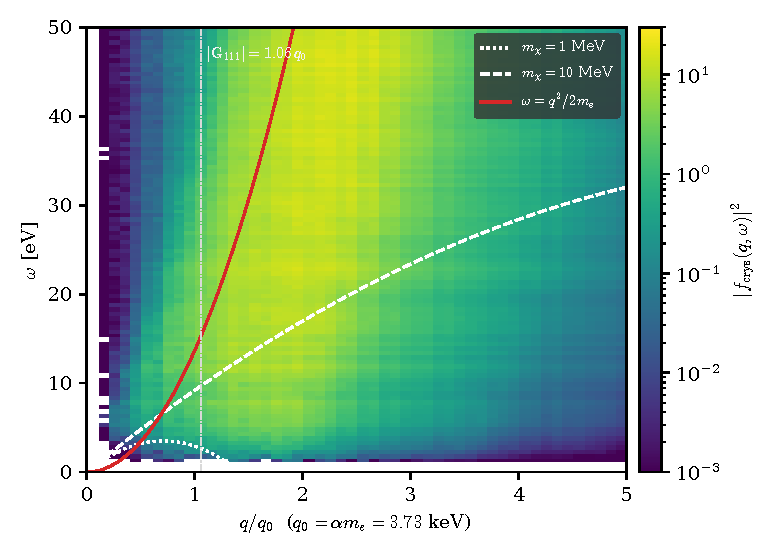
\includegraphics[width=0.85\linewidth]{figures/ch10/fig10_1.pdf}
  \caption{Crystal form factor $|f_{\mathrm{crys}}(q,\omega)|^2$ of silicon, \cref{eq:10.1-fcrys}, from the tabulation of Ref.~\cite{essig2016direct}: PBE bands with the gap set to \SI{1.11}{eV} by a scissor shift, valence to conduction, unscreened, averaged over the directions of $\vect{q}$. For display, bins are merged to $0.1\,q_0$ in $q$ and \SI{0.5}{eV} in $\omega$; white cells below $0.3\,q_0$ are bins that the grid of crystal momenta of the calculation does not reach, and white cells in the lowest row are bins next to the gap that hold no weight. White curves: the largest energy that dark matter of 1 and \SI{10}{MeV} can deposit at each $q$, $qv_{\mathrm{max}} - q^2/2\mchi$ with $v_{\mathrm{max}} = \SI{794.5}{km.s^{-1}}$ (\cref{eq:1.3-region}); everything below a curve is kinematically allowed. Red: the free-electron recoil $\omega = q^2/2m_e$, along which the weight concentrates at large $q$. Dash-dotted: $|\vect{G}_{111}| = \sqrt3\,2\pi/a = 1.06\,q_0$, the shortest reciprocal-lattice vector. The color scale is logarithmic.}\label{fig:10-fcrys}
\end{figure}

Divided by $\pi\nd_eq^2/m_e$ with the valence density $\nd_e = 8/\Omega$, the first moment of the tabulated $\bar S^0$ over its \SI{50}{eV} is 1.03 at $q_0$, and 1.1 to 1.2 between $0.3\,q_0$ and $0.7\,q_0$, as means over windows of $0.2\,q_0$ with the bins the grid does not reach counted as zero. The scissor shift raises the first moment, since it moves every transition up by about \SI{0.55}{eV} without changing its weight; that is the difference between the PBE gap of silicon (\cref{sec:3.4}) and \SI{1.11}{eV}. At small $q$, where the mean energy deposited is a few eV, the shift accounts for about ten percent; the rest of the excess has no identified cause (\cref{sec:10.10-manybody}). Beyond $1.5\,q_0$ the ratio falls, to 0.83 at $1.5\,q_0$ and 0.33 at $2\,q_0$: the free recoil energy is then 31 and \SI{54}{eV}, and the weight has moved past the last tabulated band. As a second check, the tabulated $\bar S^0$ at $q_0$ lies within 25 percent of the independent-particle structure factor of the local empirical pseudopotential of \cref{we:8-lf-nuisance}, along $[100]$, between 5 and \SI{20}{eV}. The two calculations share no input other than the crystal structure.

The form factor varies with $q$ on two scales that silicon happens to have in common, the zone scale and $q_0$ (\cref{sec:1.3}). At momentum transfers small compared with the zone, $2\pi/a = 0.61\,q_0$, the vertex reduces to its optical limit, $\rho_{cv} \simeq \vect{q}\cdot\vect{v}_{cv}/(\varepsilon_{c\vect{k}} - \varepsilon_{v\vect{k}})$ (\cref{sec:3.2}), so $\bar S^0 \propto q^2$ at fixed $\omega$, and by \cref{eq:A.8-fcrys} $|f_{\mathrm{crys}}|^2 \simeq q^5\Omega\varepsilon_2(\omega)/8\pi^2\alpha^2m_e^2$ with the optical $\varepsilon_2$. Integrated over energy, the tabulated form factor grows as $q^{4.8}$ between $0.3\,q_0$ and $0.75\,q_0$, close to this dipole scaling even where $q$ is no longer small compared with the zone. Near $|\vect{G}_{111}| = 1.06\,q_0$ the momentum transfer resolves the bond, the optical limit fails, and the vertex is set by the plane-wave content of the valence states at momenta of order $q$ (\cref{eq:3.2-rhopw}). At fixed $\omega$ between 3 and \SI{10}{eV}, $|f_{\mathrm{crys}}|^2$ peaks at $1.7$ to $1.8\,q_0$ and at $2\,q_0$ it is still 2.1 to 2.5 times its value at $q_0$; by $3\,q_0$ it has fallen to a quarter of its value at $q_0$. The factor $q^3$ in \cref{eq:10.1-fcrys} pushes this peak outward. The rate weight of \cref{eq:10.1-rateiso}, $q\bar S^0$, peaks earlier, at 1.1 to $1.4\,q_0$.

At large $q$ the figure shows where the weight goes. Along the red curve, $\omega = q^2/2m_e$, a dark-matter particle would give a free electron at rest its recoil energy, and at large $q$ the response of bound electrons gathers around it, broadened by their momenta, as in the impulse approximation of \cref{we:4-gas}. At a fixed small energy deposited, a large $q$ needs an electron that already moves against the momentum transfer with a momentum of about $q/2$, and the bound valence states have little weight at momenta much above $q_0$. That is why, integrated over the tabulated energies, $|f_{\mathrm{crys}}|^2$ falls as $q^{-5}$ between 2 and $4\,q_0$. The white curves show which part of the plane the halo can reach. Dark matter of \SI{1}{MeV} reaches only a thin sliver above the gap at $q < 1.4\,q_0$, near the bottom of the figure; at \SI{10}{MeV} it reaches deposits up to \SI{35}{eV} and momentum transfers well past the peak of $|f_{\mathrm{crys}}|^2$.

\begin{workedexample}{The silicon rate at \SI{10}{MeV}}\label{we:10-rate}
Take $\mchi = \SI{10}{MeV}$, $\sigmae = \SI{e-37}{cm^2}$ and the standard halo of \cref{app:A.8}: $\rho_\chi = \SI{0.3}{GeV.cm^{-3}}$, $v_0 = \SI{238}{km.s^{-1}}$, $v_{\mathrm{esc}} = \SI{544}{km.s^{-1}}$ and $v_{\mathrm{E}}^{\mathrm{ref}} = \SI{250.5}{km.s^{-1}}$. The reduced mass is $\mu_{\chi e} = \SI{486.2}{keV}$, so $m_e^2/\mu_{\chi e}^2 = 1.105$, and the number density is $\rho_\chi/\mchi = \SI{30}{cm^{-3}}$. The prefactor of the box, with $M_{\mathrm{cell}} = \SI{52.33}{GeV}$, is
\begin{equation*}
  \frac{\rho_\chi\,\sigmae\,\alpha\,m_e^2}{\mchi\,M_{\mathrm{cell}}\,\mu_{\chi e}^2}
  = \frac{\SI{30}{cm^{-3}}\times\SI{e-37}{cm^2}\times c\times1.105}{137.036\times M_{\mathrm{cell}}}
  = \SI{2.45e5}{kg^{-1}.yr^{-1}} ,
\end{equation*}
where the factor $c$ turns $\rho_\chi\sigmae/\mchi$ into a rate and $\eta$ is then a pure number, $\langle1/v\rangle = 1041$ in units of $1/c$. Everything else is the double integral of $\eta\FDM^2|f_{\mathrm{crys}}|^2\,\dd q\,\dd\omega/q^2$ over the tabulated bins, with $\vmin = \omega/q + q/2\mchi$ and $\eta$ in the closed form of \cref{app:D.1}.

For a heavy mediator, $\FDM = 1$, the double integral is 0.652, and the rate above the gap is
\begin{equation*}
  \mathcal{R} = \SI{2.45e5}{kg^{-1}.yr^{-1}}\times0.652 = \SI{1.60e5}{kg^{-1}.yr^{-1}} ,
\end{equation*}
about 440 events per kilogram and day. The spectrum $\dd\mathcal{R}/\dd\omega$ peaks at \SI{6.5}{eV}, its mean is \SI{6.0}{eV}, 38 percent of the events deposit at most \SI{4.9}{eV}, and it ends at \SI{35}{eV}, the largest energy a particle at $v_{\mathrm{max}}$ can deposit. At the peak energy the integrand in $q$ is flat between about $1.7\,q_0$ and $1.9\,q_0$ (6.5 to \SI{7.09}{keV}); only 5 percent of the rate comes from $q < q_0$, and 27 percent from $q > 2\,q_0$.

For a light mediator, $\FDM = (q_0/q)^2$, the integral is 0.193, and $\mathcal{R} = \SI{4.73e4}{kg^{-1}.yr^{-1}}$, about 130 per kilogram and day. The factor $(q_0/q)^4$ moves the rate to small $q$ and low energy: the spectrum peaks at \SI{3.3}{eV}, its mean is \SI{4.5}{eV}, 66 percent of the events deposit at most \SI{4.9}{eV}, and the $q$ integrand at the peak is largest near $0.6\,q_0 = \SI{2.2}{keV}$, near the kinematic edge. Now 44 percent of the rate comes from $q < q_0$.

The two mediators probe different parts of \cref{fig:10-fcrys}. The heavy mediator samples the form factor near its maximum, at twice $q_0$ and a few eV, where the bands and the plane-wave content of the valence states set the answer. The light mediator samples its small-$q$ edge, where the form factor is smallest and where, as the limit check shows, screening matters most. The scaling of \cref{eq:1.5-heuristic} gives the rest: at fixed $\sigmae$ the rate falls as $1/\mchi$ once $\mchi$ is well above the threshold and the reach in $q$ covers the peak. Published rates differ from these numbers mainly through the halo: Ref.~\cite{essig2016direct} uses $\rho_\chi = \SI{0.4}{GeV.cm^{-3}}$, $v_0 = \SI{230}{km.s^{-1}}$, $v_{\mathrm{esc}} = \SI{600}{km.s^{-1}}$ and an Earth speed of \SI{240}{km.s^{-1}}~\cite[Sect.~6]{essig2016direct}.
\end{workedexample}

\subsection{Convergence parameters and omitted physics}

A crystal form factor is computed from Kohn--Sham bands and plane-wave vertices. The bands come from a density-functional calculation with a pseudopotential (\cref{sec:3.4,sec:3.5}), with the gap set by a scissor shift or by quasiparticle corrections (\cref{app:E.1,app:E.3}). The vertex is the plane-wave overlap \cref{eq:3.2-rhopw}, evaluated for every valence state, every conduction state and every Umklapp vector that a given $\vect{q}$ requires, with $\vect{q}$ kept unfolded. \Cref{app:E.7} sets out the calculation and its cost, about $5\times10^{11}$ vertices for silicon with 52 conduction bands and momentum transfers up to \SI{30}{keV}. The plane-wave cutoff limits the largest $q$ a vertex can carry, the number of conduction bands the largest $\omega$, and the grid of crystal momenta the resolution at small $q$ and near the onset; the white cells of \cref{fig:10-fcrys} are this last limit. At large $q$ the pseudopotential matters as well. A pseudo-wavefunction is smooth inside the core region by construction, and above a few $q_0$ the vertex needs the nodes of the true valence states near the nucleus. The all-electron reconstruction of \cref{app:E.2} restores them; Griffin and collaborators found that it raises the valence-to-conduction rate of germanium at energies above about \SI{15}{eV}~\cite[Sect.~1]{griffin2021extended}. For silicon at \SI{10}{MeV}, \cref{we:10-rate} draws a quarter of the heavy-mediator rate from $q > 2\,q_0$, and that part rests on the same correction.

Its place in the expansion hierarchy, $\mathfrak{T}_0$, fixes what the calculation leaves out. It has no screening: the dark matter's potential acts on independent electrons, while in the crystal the other electrons polarize and reduce it, most strongly at small $q$, where the light mediator and the lightest masses collect their rate. \Cref{sec:10.2} adds the random-phase screening and the local fields, and shows when the loss function gives the rate exactly. It has no electron--hole attraction: an exciton moves weight from the continuum toward the gap, which matters for the lowest thresholds, and \cref{sec:10.5} treats excitons at finite momentum. It has no lattice: the nuclei are clamped, so the phonon-assisted transitions that open the indirect gap below the zero-phonon edge (\cref{sec:13.1}) and the Migdal effect (\cref{chap:12}) are absent. It holds only valence-to-conduction transitions: the $2p$ shell of silicon, \SI{99}{eV} below the valence maximum, and the $3d$ shell of germanium, about \SI{29}{eV} below it, are the subject of \cref{sec:10.6}, and the table ends at the highest conduction band it includes. And it is an angle average at zero temperature, which drops the daily modulation and the thermal shift of the gap.

\section{Screening and the loss-function rate}\label{sec:10.2}

At a momentum transfer of \SI{2}{keV} the static dielectric function of silicon is about 2.9, and a potential that varies on that scale reaches the valence electrons weakened by $1/|\varepsilon|^2 \approx 0.12$. Yet the screened rate of a \SI{10}{MeV} particle with a heavy mediator is only 2.3 times smaller than the unscreened rate of \cref{sec:10.1}. The rate is an integral over all the momentum transfers and energies that kinematics allows, most of which lie where the medium screens little, and over a spectrum whose total weight screening cannot change. Two sum rules of the loss function bound it from above, with only the plasma frequency and the static dielectric function as input. The bound on the static step fails for a mediator that couples to electrons alone once the lattice is free to move, because the electrons that follow the nuclei add an acoustic peak.

\subsection{The loss-function rate}\label{sec:10.2-rate}

A mediator that couples to the electron number acts on one row of the master formula, the density $n_e(\vect{q})$, with $\mathfrak{D}_{ee} = |\tilde V(\vect{q})|^2 = \pi\sigmae\FDM(q)^2/\mu_{\chi e}^2$ (\cref{eq:1.4-Vsq}), and the spectrum \cref{eq:8.2-spectrum} needs only the structure factor $S_{ee}$. \Cref{sec:10.1} computed it for independent electrons. The exact structure factor follows from the fluctuation--dissipation theorem as $S = (2q^2/e^2)\,L/(1 - \ee^{-\beta\omega})$, with $L(\vect{q},\omega) = \Imag[-(\varepsilon^{-1})_{\vect{0}\vect{0}}(\vect{q},\omega)]$ the loss function of \cref{eq:4.4-SL}, and the exactness theorem \cref{eq:8.4-exact} says for which couplings this holds. For a dark photon, or any mediator that couples to the total charge $n_Z$, it holds at every $(\vect{q},\omega)$ with the loss function of the total dielectric matrix of electrons and nuclei. For a mediator that couples to electrons and not to nucleons it holds exactly only with the nuclei clamped. Above the phonon band the nuclei reach the electronic final states through the Migdal amplitudes alone, suppressed by powers of $\kappa_{\mathrm{BO}}$, and the loss function gives the electron-only rate to that accuracy (\cref{sec:8.4-exact}). An electron--hole pair in silicon costs at least \SI{1.17}{eV}, eighteen times the top of the phonon band, so for the electronic rate the two couplings share one formula. In silicon the Born charges vanish, and the ionic part of the total dielectric function at these energies is negligible.

Inserting $S$ into \cref{eq:8.2-spectrum}, with $e^2 = 4\pi\alpha$, gives $|\tilde V|^2 S = \sigmae\FDM^2q^2L/[2\alpha\mu_{\chi e}^2(1 - \ee^{-\beta\omega})]$ under the integrals~\cites[Eq.~(13)]{knapen2021dark}[Eq.~(1)]{hochberg2021determining}. For an isotropic target, or a crystal whose loss function is averaged over the directions of $\vect{q}$, the velocity integral and the angular integral act on the delta function alone and produce the measure $q\,\dd q\,\eta(\vmin)/4\pi^2$ of \cref{eq:A.8-eta}, with $\vmin = \omega/q + q/2\mchi$ from \cref{eq:1.3-vmin}. Collecting the factors,
\begin{keyresult}[Loss-function rate]
\begin{equation}
  \frac{\dd\mathcal{R}}{\dd\omega} = \frac{\rho_\chi\,\sigmae}{8\pi^2\alpha\,\rho_T\,\mchi\,\mu_{\chi e}^2}\int\dd q\;q^3\,\eta\bigl(\vmin(q,\omega)\bigr)\,\FDM(q)^2\,\frac{\bar L(q,\omega)}{1 - \ee^{-\beta\omega}} ,
  \label{eq:10.2-rate}
\end{equation}
with $\bar L$ the loss function averaged over the directions of $\vect{q}$. It is exact for a coupling to the total charge, and for a coupling to the electron density at clamped nuclei or above the phonon band to Migdal order.
\end{keyresult}
\noindent At the temperatures of a detector $\beta\Eg$ is of order $10^4$ or more, and the factor $1/(1 - \ee^{-\beta\omega})$ is one. All of the medium's physics is now in one measurable function. Screening is in it through the inverse of the dielectric matrix, and so are the local fields, because $L$ is a diagonal element of $\varepsilon^{-1}$ and not the inverse of a diagonal element of $\varepsilon$. For a momentum transfer beyond the first zone the element is the one at the reciprocal vector $\vect{G}_q$ of the unreduced $\vect{q} = \vect{q}_r + \vect{G}_q$, $L = \Imag[-(\varepsilon^{-1})_{\vect{G}_q\vect{G}_q}(\vect{q}_r,\omega)]$. A crystal has a loss function that depends on the direction of $\vect{q}$, and a rate at a fixed time keeps the full kernel of \cref{app:A.8} in place of $\eta/2q$. In a cubic crystal the first anisotropic term of $L$ has angular momentum four, and it is the source of the daily modulation of \cref{sec:11.7}.

The rate of \cref{sec:10.1} is the same formula with $L$ replaced by $\varepsilon_2$ of the independent-particle head: since $S^{\mathrm{IP}} = -2\Imag R^0_{\vect{0}\vect{0}}$ (\cref{sec:10.1}) and $\varepsilon_2 = -v_{\mathrm{C}}(q)\Imag R^0_{\vect{0}\vect{0}}$ (\cref{eq:4.6-R0}), $S^{\mathrm{IP}} = (2q^2/e^2)\,\varepsilon_2^{\mathrm{IP}}$. The prefactor is the one of \cref{eq:10.2-rate}, and \cref{eq:10.1-fcrys} is this relation rewritten as a form factor. Each many-body approximation of \cref{sec:4.6} is then a choice of what to put in place of $\bar L$. Independent particles put $\varepsilon_2^{\mathrm{IP}}$. The random-phase approximation without local fields puts $\varepsilon_2^{\mathrm{IP}}/|\varepsilon_{\vect{0}\vect{0}}|^2$, in which the head $\varepsilon_{\vect{0}\vect{0}} = 1 - v_{\mathrm{C}}(q)R^0_{\vect{0}\vect{0}}$ is inverted as a number. With local fields it is $\Imag[-(\varepsilon^{-1})_{\vect{0}\vect{0}}]$ with the full matrix of \cref{eq:4.6-rpaLF}. Exchange--correlation kernels and the electron--hole attraction change the proper response inside the same inverse (\cref{sec:4.6,sec:4.9}). The three rates differ only in the many-body approximation $\mathcal{X}$ of \cref{sec:8.5}, IP, RPA and RPA + LF, with every other entry of $\mathfrak{T}$ at its base value.

For a dark photon, \cref{eq:10.2-rate} uses the reference cross section with the vacuum mixing $\zeta$, and the loss function already contains the in-medium mixing. In scattering the dark photon mixes with the longitudinal photon of the medium, its propagator acquires the factor $1/\varepsilon(\vect{q},\omega)$, and that factor is the screening of the total-charge row (\cref{sec:8.4-mixing}). The vacuum mixing goes with the full response and the in-medium mixing with the proper one; multiplying \cref{eq:10.2-rate} by $\zeta_{\mathrm{eff}}^2/\zeta^2$ would count the screening twice.

The loss function is computed from Kohn--Sham states: the random-phase dielectric matrix with local fields is inverted at each $(\vect{q}_r,\omega)$, and the diagonal element is read off at $\vect{G}_q$ (\cref{app:E.6}). Two kinds of measurement test it: optical constants give $L$ at $q \to 0$, the curve of \cref{fig:4-siloss}, and electron energy-loss and inelastic x-ray scattering give it at finite $q$. The silicon tables used below are a published calculation of this kind~\cite{knapen2021dark}, distributed with the DarkELF code~\cite{knapen2022darkelf}. They use Kohn--Sham states with the gap fixed by a scissor shift, a $\vect{k}$ grid of $8^3$ and 70 bands, and give the dielectric matrix with and without local fields. They extend to $q = \SI{22.5}{keV}$ and $\omega = \SI{89}{eV}$. Kinematics keeps the rate inside them, since $\omega \le qv_{\mathrm{max}}$ is below \SI{60}{eV} for every momentum of the table. For a material without such tables, the Mermin oscillator method of \cref{sec:4.5} fits the measured optical loss function, gap and absorption peaks included, and carries each term to finite $q$ with its share of the $f$-sum. For silicon it agrees with the first-principles tables to within 10 percent in the rate above a two-electron threshold, and the uncertainty grows for masses whose rate lies near the gap~\cite[App.~C]{knapen2021dark}.

\begin{limitbox}[Loss-function rate][lim:10.2a]
For a coupling to the electron density or to the total charge, the spectrum per unit target mass is $\dd\mathcal{R}/\dd\omega = [\rho_\chi\sigmae/(8\pi^2\alpha\rho_T\mchi\mu_{\chi e}^2)]\int\dd q\,q^3\eta(\vmin)\FDM^2\,\Imag[-1/\varepsilon(q,\omega)]/(1 - \ee^{-\beta\omega})$~\cites[Eqs.~(6) and (13)]{knapen2021dark}[Eq.~(1)]{hochberg2021determining}.
\par\smallskip
{\centering
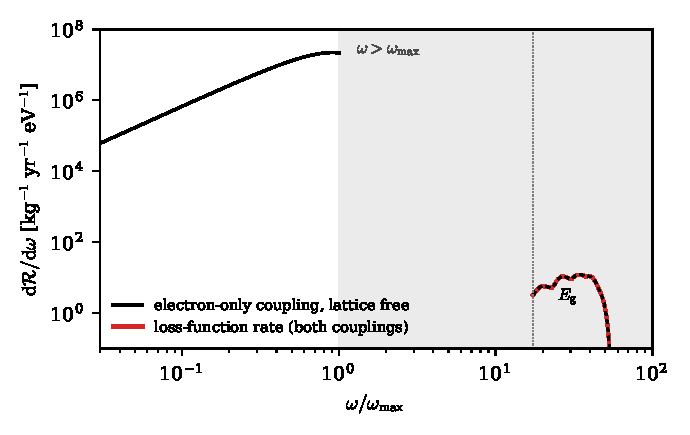
\includegraphics[width=0.82\linewidth]{figures/ch10/limit10_2a.pdf}
\captionof{figure}{Spectrum of silicon at $\mchi = \SI{1}{MeV}$, heavy mediator, $\sigmae = \SI{e-37}{cm^2}$, against $\omega/\omega_{\max}$, with $\omega_{\max} = \SI{64.1}{meV}$ the top of the phonon band. Red: the loss-function rate with the random-phase loss function with local fields; it is the whole rate of a dark photon, since the Born charges of silicon vanish. Black: an electron-only coupling with the lattice free to move, which adds the acoustic peak carried by the electrons that follow the nuclei. Model of the peak: isotropic linear longitudinal branch with $c_{\mathrm{LA}} = \SI{8.43}{km/s}$ up to $|\vect{q}| = 2\pi/a$, 14 electrons per atom following rigidly, no Debye--Waller factor, no Umklapp, transverse or multiphonon terms. Gray: $\omega > \omega_{\max}$, where the two couplings share the loss-function rate; dotted, the gap.}\label{fig:10-elf-limit}
\par}
\smallskip
Inside the phonon band an electron-only coupling excites acoustic phonons through the electrons that move with the nuclei, a peak that the loss function of the total charge does not have and that, in this model, carries more than $10^4$ times the electronic rate.
\end{limitbox}

\subsection{Screening corrections in silicon}\label{sec:10.2-corrections}

\Cref{fig:10-screening} shows the silicon rate in the three approximations. At \SI{10}{MeV} with a heavy mediator the spectrum peaks near \SI{5}{eV} in each of them, and only its height changes. Per kilogram-year at $\sigmae = \SI{e-37}{cm^2}$ the total above the gap is $1.36\times10^5$ events for independent particles, from the independent-particle head of these tables and not from the form-factor table of \cref{sec:10.1}, which gives $1.60\times10^5$ (\cref{sec:10.10-manybody} traces the difference), $8.6\times10^4$ in the random-phase approximation without local fields and $5.9\times10^4$ with them. The ratio of the unscreened rate to the screened one with local fields is 2.3 for a heavy mediator and 3.7 for a light one, and above about \SI{10}{MeV} it hardly depends on the mass. Below a few MeV it rises steeply, to 9 and 13 at \SI{1}{MeV}. At \SI{3}{MeV} it is 2.8 for a heavy mediator and 5.1 for a light one: random-phase screening lowers the independent-particle rate by \SI{52}{\percent}, and local fields lower what remains by a further \SI{26}{\percent}; for a light mediator the steps are \SI{76}{\percent} and \SI{18}{\percent}. The local fields alone lower the rate by a factor 1.46 for a heavy mediator and 1.27 for a light one at \SI{10}{MeV}, and by about 1.1 at \SI{1}{MeV}.

\begin{figure}[tbp]
  \centering
  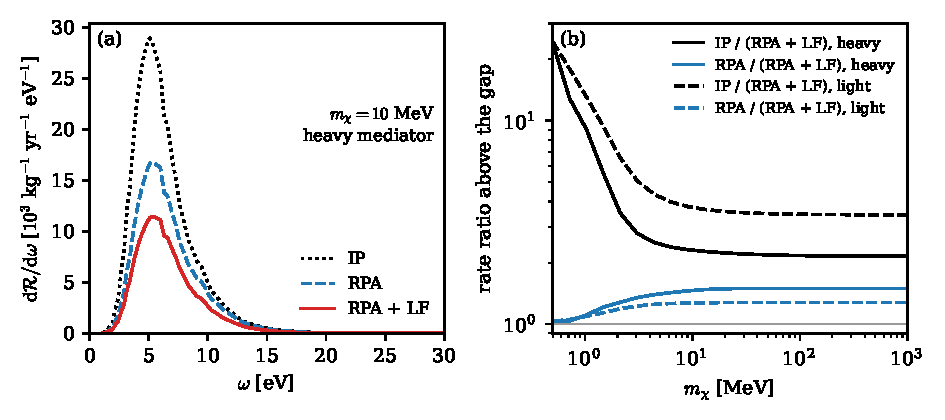
\includegraphics[width=\linewidth]{figures/ch10/fig10_2.pdf}
  \caption{Electron-recoil rate of silicon in three approximations, independent particles, RPA, and RPA with local fields, from the random-phase dielectric matrices of Knapen, Kozaczuk and Lin~\cite{knapen2021dark}, with and without local fields, with $\rho_\chi = \SI{0.3}{GeV.cm^{-3}}$, the standard halo of \cref{sec:1.2}, $\sigmae = \SI{e-37}{cm^2}$ and threshold \SI{1.11}{eV}, the step-model gap of pair creation that accompanies the tables (their scissor puts the gap at \SI{1.17}{eV}). IP: $\varepsilon_2$ of the independent-particle head of the same tables in place of $L$, the unscreened rate of \cref{sec:10.1} from a different tabulation; RPA: $\varepsilon_2/|\varepsilon_{\vect{0}\vect{0}}|^2$; RPA + LF: $\Imag[-(\varepsilon^{-1})_{\vect{0}\vect{0}}]$. The tabulated functions are averaged over the directions of $\vect{q}$ in bins of \SI{100}{eV} in $|\vect{q}|$, a choice of this figure, and end at $|\vect{q}| = \SI{22.5}{keV}$; momenta above \SI{15}{keV} already carry less than \SI{2}{\percent} of the rate at \SI{10}{MeV}. (a) Spectra at $\mchi = \SI{10}{MeV}$, heavy mediator. (b) Ratio of the rate above the gap to the rate with local fields, against $\mchi$; solid, heavy mediator, $\FDM = 1$; dashed, light mediator, $\FDM = (q_0/q)^2$.}
  \label{fig:10-screening}
\end{figure}

A pointwise screening factor would suggest a larger effect. The static values of the same tables give $\varepsilon(q,0) = 2.87$ at \SI{2}{keV} and 1.76 at $q_0 = \SI{3.73}{keV}$, so $1/\varepsilon^2$ is 0.12 and 0.32. At finite frequency the factor is stronger still: at $q_0$ the ratio $\varepsilon_2^{\mathrm{IP}}/L$ is 4.7 at \SI{3}{eV}, 5.2 at \SI{5}{eV} and 4.4 at \SI{10}{eV}. A pointwise factor leaves out where in $q$ the rate comes from, the $f$-sum rule, and the local fields, and these set the rate ratio of 2.3.

Consider first which momentum transfers carry the rate. With a heavy mediator, $q^3\eta(\vmin)$ weights large momentum transfers until the kinematic edge closes them, and at \SI{10}{MeV} half of the screened rate comes from $q > \SI{6.7}{keV}$ and \SI{29}{\percent} from $q > 2q_0$. There the valence electrons barely screen. At \SI{8}{keV} the static factor is 0.87, and the head screening, the ratio of the independent-particle rate to the random-phase rate without local fields at that momentum, is 1.18, against 13 at \SI{2}{keV} and 4.2 at $q_0$. A light mediator weights the small momenta, where screening is strong, and its ratio is correspondingly larger.

The $f$-sum rule is the second. Screening does not remove spectral weight, since $\int\dd\omega\,\omega L$ and $\int\dd\omega\,\omega\varepsilon_2$ are both $(\pi/2)\omega_p^2$ at every $\vect{q}$ (\cref{eq:4.4-fsumL,eq:4.4-fsumeps}); it moves the weight from the transition energies up toward the plasmon. At $q_0$ the peak of $\varepsilon_2^{\mathrm{IP}}$ lies at \SI{14}{eV} and that of $L$ at \SI{26}{eV}. Whether the moved weight is lost depends on the largest energy the dark matter can deposit, $\mchi v_{\mathrm{max}}^2/2$. At \SI{10}{MeV} this is \SI{35}{eV}, the moved weight stays mostly in reach, and the mean energy of the heavy-mediator spectrum rises only from 6.2 to \SI{6.6}{eV}. At \SI{1}{MeV} it is \SI{3.5}{eV}, the rate samples only the depleted low-energy side of $L$, and the ratio grows to 9. This is why the curves of \cref{fig:10-screening}b turn up at small mass.

The local fields are the third, and at the momenta that carry the heavy-mediator rate they are larger than the head screening. Per unit momentum transfer, the rate without local fields exceeds the rate with them by 1.17 at $q_0$, 1.67 at \SI{8}{keV} and 1.83 at \SI{10}{keV}, two to three times the shortest reciprocal-lattice vector $|\vect{G}_{111}| = \SI{3.95}{keV}$. The reason is the crystal potential. A density wave at $\vect{q} = \vect{q}_r + \vect{G}_q$ induces, through the Bloch states, charge at every $\vect{q}_r + \vect{G}$, including the long-wavelength component at $\vect{q}_r$ itself, whose Coulomb field $v_{\mathrm{C}}(|\vect{q}_r|)$ is large and acts back. The head-only random-phase approximation keeps only the diagonal element and misses this field; the inverse of the full matrix contains it. An all-electron calculation with local fields finds the same suppression of the structure factor above about $3\alpha m_e$, and a reduction of the projected reach by 20 to \SI{50}{\percent} for masses above a few MeV~\cite{dreyer2026all}. The size is not settled. At \SI{10}{keV} the energies below \SI{89}{eV} hold only \SI{17}{\percent} of the $f$-sum, the rest lying near the free recoil at $q^2/2m_e = \SI{98}{eV}$ and above. The rate samples the far low-energy tail of the spectrum, and the tail is sensitive to the band count and the pseudopotential. The spread between published calculations at these momenta is part of the many-body uncertainty of the rate (\cref{sec:8.8}). A local empirical pseudopotential that shares no input with the tables but the crystal structure shows the same suppression (\cref{fig:10-fcrys-limit,sec:10.10-manybody}). In that model at \SI{5}{eV} the kinematic edge lies at $0.525\,q_0$; just above it, at $q = 0.55\,q_0$, screening cuts the response to 0.05 of the independent-particle value, and at $q_0$ to 0.22. Integrated over $q$, the screened rate at \SI{5}{eV} is 0.47 of the independent-particle one.

\begin{figure}[tbp]
  \centering
  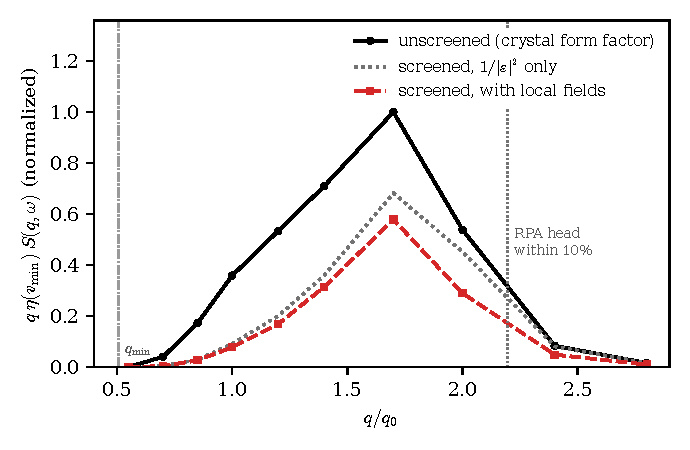
\includegraphics[width=0.85\linewidth]{figures/ch10/limit10_1a.pdf}
  \caption{Unscreened rate against screened rates in silicon at $\omega = \SI{5}{eV}$, for $\mchi = \SI{10}{MeV}$ and a heavy mediator: the rate weight $q\,\eta(\vmin)\,S(q,\omega)$ of \cref{eq:10.1-rateiso} against $q$, normalized to the maximum of the unscreened curve. All three curves come from one model, the local empirical pseudopotential of \cref{we:8-lf-nuisance} (model gap \SI{0.82}{eV}), with $\vect{q}$ along the direction $(5,3,1)$, chosen so that no $\vect{q} + \vect{G}$ comes close to zero, and spectra averaged over 4.5 to \SI{5.5}{eV}. Solid: independent particles. Dotted: random-phase screening by the macroscopic $1/|\varepsilon|^2$ alone, the leading correction. Dashed: random-phase screening with local fields over the 51 shortest reciprocal-lattice vectors, the fuller result. Dash-dotted: the smallest $q$ the halo reaches at \SI{5}{eV}. Dotted vertical: above $2.2\,q_0 = \SI{8.2}{keV}$, with $q_0 = \alpha m_e$, the macroscopic screening changes the rate by less than 10 percent. The model has no momentum components above $2.8\,q_0$, where the plot ends. Nothing is shaded. No $q$ in the plotted range brings the fuller result within 10 percent of the unscreened one.}
  \label{fig:10-fcrys-limit}
\end{figure}

The further corrections, an exchange--correlation kernel and the electron--hole attraction, change the picture mainly near the gap. An adiabatic local kernel changes the loss function by a few percent at energies of several eV, since it cannot bind an electron to a hole (\cref{sec:4.6}). The electron--hole attraction raises the spectrum within about an eV of the gap and adds bound excitons below it (\cref{sec:4.9}); \cref{sec:10.5} computes its effect on the rate. The optical limit of the tables shows what is missing at small $q$: $\varepsilon(0,0)$ is 10.2 without local fields and 9.1 with them, against the measured 11.7, the same trend as \cref{we:4-siepsinf}. A rate dominated by the region just above the gap, as for masses of a few MeV, inherits that uncertainty, and a heavier one is less sensitive to it.

\subsection{Sum-rule bounds on the rate}\label{sec:10.2-bounds}

Silicon has 28 electrons per cell, and the $f$-sum rule fixes $\int_0^\infty\dd\omega\,\omega L$ at $(\pi/2)\omega_p^2$ with $\omega_p = \SI{31.1}{eV}$ for all of them (\cref{sec:4.3}), whatever the bands, the screening or the many-body approximation. The inverse moment is fixed by the static dielectric function alone. These two integrals bound the rate of \cref{eq:10.2-rate} from above, for any material, with no calculation of the spectrum~\cites{lasenby2022dark}{barker2026first}. Define the moments of the loss function at fixed $\vect{q}$,
\begin{equation}
  K_n(\vect{q}) = \int_0^\infty\dd\omega\;\omega^n L(\vect{q},\omega) , \qquad
  K_1 = \frac{\pi}{2}\,\omega_p^2 , \qquad K_{-1} = \frac{\pi}{2}\bigl[1 - \varepsilon^{-1}(\vect{q},0)\bigr] ,
  \label{eq:10.2-moments}
\end{equation}
where $K_1$ is \cref{eq:4.4-fsumL} and $K_{-1}$ is the Kramers--Kronig relation \cref{eq:C.5-screening} at zero frequency, at which $\varepsilon^{-1}$ is real. At $\vect{q} \to 0$ in an insulator the second is the inverse moment \cref{eq:4.4-inverse}; at finite $q$ it is the static step $1 - \varepsilon^{-1}(\vect{q},0)$, which falls from 0.87 at \SI{0.5}{keV} to 0.43 at $q_0$ and 0.28 at \SI{5}{keV} in the silicon tables.

The intermediate moments follow by Hölder's inequality. For $-1 \le n \le 1$ write $\omega^nL = (\omega L)^{(1+n)/2}(L/\omega)^{(1-n)/2}$, a product of two nonnegative functions, and apply $\int fg \le (\int f^r)^{1/r}(\int g^s)^{1/s}$ with $r = 2/(1+n)$ and $s = 2/(1-n)$, so that $1/r + 1/s = 1$. Then $K_n \le K_1^{(1+n)/2}K_{-1}^{(1-n)/2}$, or
\begin{equation}
  K_n(\vect{q}) \le \frac{\pi}{2}\,\omega_p^{n+1}\bigl[1 - \varepsilon^{-1}(\vect{q},0)\bigr]^{(1-n)/2} , \qquad -1 \le n \le 1 ,
  \label{eq:10.2-Kn}
\end{equation}
which is Ref.~\cite[Eq.~(8)]{barker2026first}; the end points are the two sum rules themselves, and $n = 0$ is the Cauchy--Schwarz inequality. In the rate, the halo factor $\eta(\vmin)$ is the only other function of $\omega$. At $T = 0$ and for energies above a threshold $\omega_{\mathrm{th}}$, write $\eta \le \omega^n\eta_n^{\max}(q)$ with $\eta_n^{\max}(q) = \max_{\omega \ge \omega_{\mathrm{th}}}\omega^{-n}\eta(\vmin(q,\omega))$, extend the energy integral down to zero, which only adds positive terms since $L \ge 0$ for $\omega > 0$, and use \cref{eq:10.2-Kn}:
\begin{equation}
  \mathcal{R} \le \frac{\rho_\chi\,\sigmae\,\omega_p^{n+1}}{16\pi\alpha\,\rho_T\,\mchi\,\mu_{\chi e}^2}\int\dd q\;q^3\,\FDM(q)^2\,\eta_n^{\max}(q)\,\bigl[1 - \varepsilon^{-1}(q,0)\bigr]^{(1-n)/2} ,
  \label{eq:10.2-bound}
\end{equation}
Ref.~\cite[Eq.~(9)]{barker2026first}. The case $n = -1$ uses the static step alone and is the bound of Lasenby and Prabhu~\cite[Eqs.~(8) and (9)]{lasenby2022dark}. Every $n$ gives a valid bound, and the best one at a given mass is the smallest.

The useful form of the inverse moment needs $0 \le 1 - \varepsilon^{-1}(q,0) \le 1$. The lower limit is positivity: $1 - \varepsilon^{-1} = -v_{\mathrm{C}}R(\vect{q},0)$, and a static density response is negative by its Lehmann form (\cref{eq:4.2-positivity}). The upper limit, $\varepsilon^{-1}(\vect{q},0) \ge 0$, is not guaranteed in general, although we can show that it holds in the random-phase approximation with local fields for any insulator. The static independent-particle matrix $R^0_{\vect{G}\vect{G}'}(\vect{q},0)$ is Hermitian and negative semidefinite, each pair of states adding a positive rank-one matrix divided by minus its excitation energy, and so is $X = v^{1/2}R^0v^{1/2}$, with $v$ the diagonal matrix of $v_{\mathrm{C}}(|\vect{q}+\vect{G}|)$. The random-phase response gives $v^{1/2}Rv^{1/2} = X(1 - X)^{-1}$, whose eigenvalues $\lambda/(1 - \lambda)$, with $\lambda \le 0$, lie in $(-1, 0]$. A diagonal element of a Hermitian matrix lies between its smallest and largest eigenvalue, so $(\varepsilon^{-1})_{\vect{G}\vect{G}} = 1 + v_{\mathrm{C}}R_{\vect{G}\vect{G}}$ lies in $(0, 1]$ at every $\vect{q}$, local fields included. Beyond the random-phase approximation the same argument goes through with $R^0$ replaced by the proper response $\tilde R = (1 - R^0f_{\mathrm{xc}})^{-1}R^0$ of \cref{eq:4.6-tddft}, provided $\tilde R$ stays negative definite, that is $(-R^0)^{-1} + f_{\mathrm{xc}} > 0$. At long wavelength this is the positive inverse compressibility of \cref{eq:4.6-compress}, which the electron gas loses only near $r_s \approx 5.25$~\cite{giuliani2005quantum}, far from the $r_s \approx 2$ of the silicon valence electrons. For an arbitrary material a negative static dielectric function at finite $q$ is not excluded~\cite{dolgov1981admissible}, and the conservative replacement $1 - \varepsilon^{-1} \to 1$ that makes \cref{eq:10.2-bound} material-independent is an assumption there, not a theorem.

The bound applies to the total charge as well. For a dark photon the loss function and the static step are those of the total dielectric matrix of \cref{sec:8.4}, and the $f$-sum includes the nuclei, $\omega_p^2 + \sum_\kappa Z_\kappa^2e^2\nd_\kappa/M_\kappa$. In silicon the nuclear share is $2.73\times10^{-4}$ (\cref{sec:4.3}) and the Born charges vanish, so the numbers are those of the electrons. The inverse moment also gives a check on calculations. The unscreened $\varepsilon_2^{\mathrm{IP}}$ has $(2/\pi)\int\dd\omega\,\varepsilon_2/\omega = \varepsilon_{\vect{0}\vect{0}}(\vect{q},0) - 1$, by the Kramers--Kronig relation for $\varepsilon - 1$ (\cref{eq:C.5-KKeps}), and this exceeds the bound $1 - 1/\varepsilon_{\vect{0}\vect{0}}$ on the screened $L$ by the factor $\varepsilon_{\vect{0}\vect{0}}(\vect{q},0)$, which is 6.3 at \SI{1}{keV} in silicon.

\begin{workedexample}{The $f$-sum bound on the silicon rate at \SI{1}{MeV}}\label{we:10-fsum}
Take $\mchi = \SI{1}{MeV}$, a heavy mediator, $\sigmae = \SI{e-37}{cm^2}$, $\rho_\chi = \SI{0.3}{GeV.cm^{-3}}$ and the threshold $\omega_{\mathrm{th}} = \SI{1.11}{eV}$ of a charge detector, the step-model gap that accompanies the tables. Pairs are kinematically open for $\omega_{\mathrm{th}}/v_{\mathrm{max}} = \SI{0.42}{keV} \le q \le 2\mchi v_{\mathrm{max}} = \SI{5.30}{keV}$ and $\omega \le \mchi v_{\mathrm{max}}^2/2 = \SI{3.51}{eV}$. The screened rate of \cref{eq:10.2-rate} with local fields is 16.7 events per kilogram-year (18.5 without local fields, 157 for independent particles).

For $n = 1$, $\eta(\vmin)/\omega$ decreases with $\omega$ at fixed $q$, since $\vmin$ grows with $\omega$, so its maximum is at the threshold, $\eta_1^{\max}(q) = \eta(\vmin(q,\omega_{\mathrm{th}}))/\omega_{\mathrm{th}}$. The bound \cref{eq:10.2-bound} then needs only $\omega_p$. With all 14 electrons per atom, $\omega_p = \SI{31.1}{eV}$, it gives $7.3\times10^7$ events per kilogram-year, $4\times10^6$ times the computed rate. The valence plasma frequency, $\omega_p^{\mathrm{val}} = \SI{16.6}{eV}$, would give $2.1\times10^7$, but it is not a bound, since the core electrons hold the rest of the $f$-sum and the inequality runs over the whole spectrum. The $n = 0$ bound with the static step of the tables gives $2.0\times10^6$, and $n = -1$ gives $5.5\times10^4$, 3300 times the computed rate; with the step replaced by one it is $9.3\times10^4$. The tables contain only the valence electrons, whose step is slightly smaller than the all-electron one, so the $n = -1$ figure is a little low as a bound.

The bounds are far above the rate because they place all of the weight of $L$ at the most favorable energy, while silicon puts it where a \SI{1}{MeV} particle cannot go. The $f$-sum weight is near the plasmon, around \SI{17}{eV} at small $q$, and in the cores at hundreds of eV; the window ends at \SI{3.5}{eV}, where the gap and the screening keep $L$ small. The inverse moment weights low energies and comes closest. At \SI{10}{MeV}, with a window reaching \SI{35}{eV}, the $n = -1$ bound is 16 times the computed rate and the $f$-sum bound $8.5\times10^5$ times, both evaluated, like the rate, for $q \le \SI{22.5}{keV}$, which is valid because the bound holds at each $q$. A sum-rule bound comes close to the rate only for a material whose loss function concentrates its weight near the kinematic edge, a plasmon at a few eV, which is what the electron gas of \cref{sec:10.3} and the low-dimensional plasmons of \cref{sec:16.2} provide.
\end{workedexample}

\subsection{Static step of a relaxing lattice}\label{sec:10.2-lattice}

For a mediator that couples to electrons alone, the exact relation is $S_{ee} = (2q^2/e^2)L_e/(1 - \ee^{-\beta\omega})$ with the electron-channel function $\varepsilon_e^{-1} = 1 + v_{\mathrm{C}}R_{ee}$ (\cref{app:A.7}), and both sum rules hold for $L_e$. The $f$-sum is unchanged: the double commutator of $n_e$ with the Hamiltonian involves only the kinetic energy of the electrons (\cref{sec:4.3}), so $\int\dd\omega\,\omega L_e = (\pi/2)\omega_p^2$ with the nuclei moving, and the acoustic peak of the electron-following sector takes the share $Z_\kappa m_e/M_\kappa = 2.73\times10^{-4}$ of it in silicon (\cref{eq:8.6-fsum-e}). The static step is a different matter. With the nuclei free to move, an electron-only probe at small $q$ compresses neutral matter: the electrons it displaces drag their nuclei along, and the crystal responds as an elastic medium.

The size follows from the acoustic peak. At small $q$ a longitudinal acoustic phonon moves each cell rigidly by $\vect{U}_{\vect{R}}$, and the electrons that follow the nuclei, all $\nd_e\Omega = 28$ per cell in silicon since the Born charges vanish, give the density row the term $-\ii\,\nd_e\Omega\sum_{\vect{R}}\ee^{-\ii\vect{q}\cdot\vect{R}}\,\vect{q}\cdot\vect{U}_{\vect{R}}$ (\cref{sec:8.4-exact}). One phonon of wavevector $\vect{q}$ displaces each cell by $(2M_{\mathrm{cell}}N\omega_{\vect{q}})^{-1/2}$ along its polarization, with $N$ cells in the volume $\Vol = N\Omega$. The squared matrix element is then $N(\nd_e\Omega)^2q^2/(2M_{\mathrm{cell}}\omega_{\vect{q}})$, and
\begin{equation*}
  S_{ee}^{\mathrm{ac}}(\vect{q},\omega) = \frac{\pi\nd_e^2\Omega\,q^2}{M_{\mathrm{cell}}\,\omega_{\vect{q}}}\,\delta(\omega - \omega_{\vect{q}}) , \qquad \omega_{\vect{q}} = c_{\mathrm{LA}}q ,
\end{equation*}
at $T = 0$, with $c_{\mathrm{LA}}$ the longitudinal sound speed, the $c_\nu$ of \cref{eq:5.2-sound} for the longitudinal branch. Its first moment, $\int\dd\omega\,\omega S/2\pi = \nd_e^2\Omega q^2/2M_{\mathrm{cell}}$, is $\nd_e\Omega\,m_e/M_{\mathrm{cell}}$ times the electronic $f$-sum $\nd_eq^2/2m_e$, the share quoted above. Its inverse moment is not small. With $L_e = (e^2/2q^2)(1 - \ee^{-\beta\omega})S_{ee}$, the peak adds $(2/\pi)\int\dd\omega\,L_e^{\mathrm{ac}}/\omega = e^2\nd_e^2\Omega/(M_{\mathrm{cell}}\,\omega_{\vect{q}}^2)$ to the static step, and
\begin{keyresult}[Static step of a relaxing lattice]
\begin{equation}
  1 - \varepsilon_e^{-1}(\vect{q},0) = \bigl[1 - \varepsilon_{\mathrm{cl}}^{-1}(\vect{q})\bigr] + \mathcal{G}_{\mathrm{rel}}(\vect{q}) , \qquad
  \mathcal{G}_{\mathrm{rel}}(\vect{q}) \to \frac{\varOmega_{P,e}^2}{(c_{\mathrm{LA}}q)^2} , \quad \varOmega_{P,e}^2 = \frac{e^2\nd_e^2}{\rho_T} ,
  \label{eq:10.2-relaxed}
\end{equation}
as $q \to 0$, with $\varepsilon_{\mathrm{cl}}$ the dielectric function at clamped nuclei, $\nd_e$ the density of all the electrons and $\rho_T = M_{\mathrm{cell}}/\Omega$. The lattice term grows as $(c_{\mathrm{LA}}q)^{-2}$ in every solid, polar or not. Its general form, a sum over branches with the electron-following charge $Z^{(e)}_\kappa(\vect{q})$ of each atom, is \cref{eq:E.16-step}.
\end{keyresult}
\noindent For silicon, $\nd_e = \SI{7.00e23}{cm^{-3}}$ and $\rho_T = \SI{2.33}{g.cm^{-3}}$ give $\varOmega_{P,e} = \SI{0.51}{eV}$, and with $c_{\mathrm{LA}} = \SI{8.43}{km/s}$ along $[100]$ (\cref{app:C.18}) the lattice term equals one at $q = \SI{18}{keV}$, far beyond the zone boundary. The limiting form is derived only as $q \to 0$. At finite $q$ the dispersion bends over and the electron-following charge falls below 14 per atom, at relative order $(qa)^2$ and in opposite directions; at \SI{1}{keV} the limiting form gives $3\times10^2$, and the true value there is only estimated to exceed $10^2$ (\cref{app:E.16}). Either way the step exceeds one by orders of magnitude throughout the zone, and the bound \cref{eq:10.2-bound} with $n = -1$, and with every $n < 1$ through the power $(1 - n)/2$, fails for an electron-only coupling once the lattice relaxes. Lasenby and Prabhu noted that phonon rates of electrophilic mediators exceed the sum-rule bounds of charge couplings~\cite[Sect.~VII]{lasenby2022dark}; \cref{eq:10.2-relaxed} gives the term responsible. It is the acoustic peak of $S_{ee}$ that the exactness theorem of \cref{sec:8.4} attributed to the electrons that follow the nuclei. Its amplitude is the coefficient of $\ii\vect{q}\cdot\vect{U}$ in the density row, the coupling per unit volume $c_1^{(e)}\nd_e$ of the electrons that move with the cells; for the charge this coefficient cancels between electrons and nuclei, and the peak is absent.

The clamped bound holds in every many-body approximation, with the proviso on $\tilde R$ above; the lattice term is harmonic and adiabatic, with one phonon in the final state. For the electron-only coupling the $f$-sum bound and a restricted static-step bound survive. The $f$-sum bound holds as it stands. And for a threshold above the phonon band the electron-following sector contributes nothing to $\int_{\omega_{\mathrm{th}}}^\infty\dd\omega\,L_e/\omega$ except through Migdal amplitudes, so the clamped step bounds that integral up to corrections in powers of $\kappa_{\mathrm{BO}}$ (\cref{sec:8.6}). A detector with an electronic threshold can use the clamped bound for either coupling; a calorimeter with a threshold in the phonon band cannot use it for an electrophilic mediator.

\begin{limitbox}[Sum-rule bounds on the loss function][lim:10.2b]
For any target in its ground state, $\int_0^\infty\dd\omega\,\omega L = (\pi/2)\omega_p^2$ and $\int_0^\infty\dd\omega\,L/\omega = (\pi/2)[1 - \varepsilon^{-1}(q,0)] \le \pi/2$, and with $\eta \le \omega^n\eta_n^{\max}$ they bound the rate as in \cref{eq:10.2-bound}~\cites[Eqs.~(1), (8) and (9)]{lasenby2022dark}[Eqs.~(1), (2), (8) and (9)]{barker2026first}.
\par\smallskip
{\centering
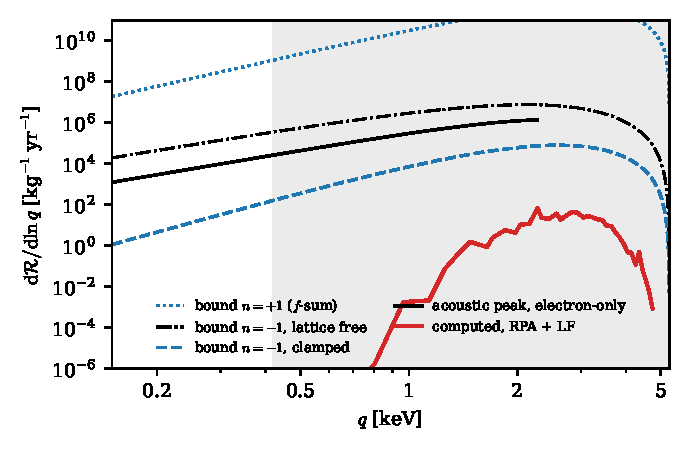
\includegraphics[width=0.82\linewidth]{figures/ch10/limit10_2b.pdf}
\captionof{figure}{Rate per unit $\ln q$ in silicon at $\mchi = \SI{1}{MeV}$, heavy mediator, $\sigmae = \SI{e-37}{cm^2}$, threshold \SI{1}{meV}, against the bounds of \cref{eq:10.2-bound}. Red: the computed electronic rate (random-phase loss function with local fields). Dashed: the clamped bound with $n = -1$ and the static step of the same tables; dotted: the $f$-sum bound, $n = 1$, $\omega_p = \SI{31.1}{eV}$. Black: the acoustic peak of an electron-only coupling, in the model of \cref{fig:10-elf-limit}; dash-dotted: the $n = -1$ bound with the lattice term \cref{eq:10.2-relaxed} added, in its limiting form $\varOmega_{P,e}^2/(c_{\mathrm{LA}}q)^2$ at every $q$ shown. Gray: momenta at which electron--hole pairs are open, $q \ge \Eg/v_{\mathrm{max}}$; there the clamped bound holds for both couplings when the threshold lies above the phonon band. The acoustic peak exceeds the clamped bound by 120 at \SI{0.5}{keV}, 42 at \SI{1}{keV} and 21 at \SI{2}{keV}.}\label{fig:10-sumrule-limit}
\par}
\smallskip
For an electron-only coupling with the lattice free to move, the static step grows as $(c_{\mathrm{LA}}q)^{-2}$ and exceeds one throughout the zone, and only the $f$-sum bound survives.
\end{limitbox}

\section{Electron-gas models and plasmons}\label{sec:10.3}

Put the Lindhard loss function of the silicon valence electrons into the rate of \cref{sec:10.2}, and a \SI{100}{MeV} particle with a heavy mediator makes $1.31\times10^4$ events per kilogram-year above \SI{1.11}{eV} at $\sigmae = \SI{e-37}{cm^2}$. The crystal tables of \cref{sec:10.2}, with bands, local fields and a gap, give $1.22\times10^4$. A model with one parameter, the electron density, comes within seven percent of the crystal rate. At \SI{1}{MeV} the same model gives 45 times the crystal rate. The gas also carries the plasmon, which at small momentum transfer holds almost the whole $f$-sum, and it is natural to ask whether dark matter can excite it. We derive the electron-gas rate and find where it agrees with silicon and why, then isolate the plasmon pole in the rate and show that halo dark matter falls short of it by about $\omega_p$ in energy and a factor of 3.5 in speed.

\subsection{The Lindhard loss-function rate}\label{sec:10.3-gas}

The electron gas of \cref{sec:4.5} is isotropic, so the direction average in \cref{eq:10.2-rate} does nothing, and its loss function in the random-phase approximation is $\Imag[-1/\varepsilon_{\mathrm{Lin}}(q,\omega)]$ with the Lindhard dielectric function of \cref{eq:4.5-rpa,eq:4.5-lindhard}. Inserting it,
\begin{keyresult}[Electron-gas loss-function rate]
\begin{equation}
  \frac{\dd\mathcal{R}}{\dd\omega} = \frac{\rho_\chi\,\sigmae}{8\pi^2\alpha\,\rho_T\,\mchi\,\mu_{\chi e}^2}\int\dd q\;q^3\,\eta\bigl(\vmin(q,\omega)\bigr)\,\FDM(q)^2\,\Imag\!\left[\frac{-1}{\varepsilon_{\mathrm{Lin}}(q,\omega)}\right] ,
  \label{eq:10.3-gasrate}
\end{equation}
at $T = 0$, with $\varepsilon_{\mathrm{Lin}}$ fixed by the electron density alone through $k_{\mathrm{F}}$ and $\omega_p$. The Mermin form replaces $\varepsilon_{\mathrm{Lin}}$ by $\varepsilon_{\mathrm{Mer}}$ of \cref{eq:4.5-mermin}.
\end{keyresult}
\noindent This is the rate of Knapen, Kozaczuk and Lin with their Lindhard and Mermin functions~\cite[Eqs.~(13), (17) and (19)]{knapen2021dark}. Their prefactor $3\omega_p^2/q^2v_{\mathrm{F}}^2$ is the $k_{\mathrm{TF}}^2/q^2$ of the static Lindhard screening $\varepsilon = 1 + (k_{\mathrm{TF}}^2/q^2)F_{\mathrm{L}}$ (\cref{eq:4.5-static}), since $k_{\mathrm{TF}}^2 = 2e^2\mathcal{N}_{\mathrm{F}} = e^2m_ek_{\mathrm{F}}/\pi^2$ and $\omega_p^2 = e^2k_{\mathrm{F}}^3/3\pi^2m_e$ give $k_{\mathrm{TF}}^2 = 3\omega_p^2/v_{\mathrm{F}}^2$, and their bracket $f^{\mathrm{L}}_1 + \ii f^{\mathrm{L}}_2$ is $-R^0/2\mathcal{N}_{\mathrm{F}}$, the braced expression of \cref{eq:4.5-lindhard}. For silicon the density is that of the four valence electrons per atom, $r_s = 2.0$, $k_{\mathrm{F}} = \SI{3.57}{keV}$ and $\omega_p = \SI{16.6}{eV}$ (\cref{we:4-siplasmon}). Below $q_{\mathrm{c}}$ the gas also has the undamped plasmon of \cref{eq:4.5-plasmonL}, a delta function in $\omega$; we return to it in \cref{sec:10.3-pole} and leave it out of \cref{eq:10.3-gasrate} for now, since halo dark matter cannot reach it.

The comparison with silicon uses the random-phase tables with local fields of \cref{sec:10.2}. Both rates are integrated on the momenta of those tables, from 0.49 to \SI{22.5}{keV}, above the threshold $\Eg = \SI{1.11}{eV}$, the step-model gap that accompanies the tables; their scissor puts the gap at the physical low-temperature value, \SI{1.17}{eV}. Per kilogram-year at $\sigmae = \SI{e-37}{cm^2}$:
\begin{center}
\begin{tabular}{@{}lcccccc@{}}
\toprule
& \multicolumn{2}{c}{\SI{1}{MeV}} & \multicolumn{2}{c}{\SI{10}{MeV}} & \multicolumn{2}{c}{\SI{100}{MeV}} \\
& heavy & light & heavy & light & heavy & light \\
\midrule
Silicon, RPA + LF & 16.7 & 90 & $5.89\times10^4$ & $9.8\times10^3$ & $1.22\times10^4$ & $1.62\times10^3$ \\
Lindhard / silicon & 45 & 70 & 1.42 & 2.6 & 1.07 & 2.1 \\
Mermin / silicon & 54 & 94 & 1.57 & 2.9 & 1.21 & 2.4 \\
\bottomrule
\end{tabular}
\end{center}
The Mermin rows use one term with $\gamma_{\mathrm{rel}} = \SI{3.66}{eV}$, the width of the measured silicon loss peak, which is a fit parameter and not a collision rate (\cref{sec:4.5}).

The gas lacks the gap of silicon and the high-momentum tail of its bound electrons, two errors of opposite sign that set these ratios and that the spectrum of \cref{fig:10-gas-limit} shows. The first is the gap. The gas is a metal. Its continuum reaches down to $\omega = 0$, where $L \simeq e^2m_e^2q\omega/2\pi k_{\mathrm{TF}}^4$ (\cref{sec:4.5}), while silicon has no pairs below its gap and weak absorption up to its peaks at 3.4 and \SI{4.2}{eV} (\cref{fig:4-siloss}). At \SI{100}{MeV} with a heavy mediator the gas spectrum exceeds the crystal one by a factor 24 at \SI{2}{eV} and 4.2 at \SI{3}{eV}. A particle of \SI{1}{MeV} deposits at most $\mchi v_{\mathrm{max}}^2/2 = \SI{3.5}{eV}$ (\cref{eq:1.3-omegamax}), so it samples only this region, and the gas overestimates its rate by a factor 45.

The second error is the momentum distribution of the electrons. The halo deposits at most $\omega = qv_{\mathrm{max}}$ at momentum $q$. In the gas the pairs at $q > 2k_{\mathrm{F}}$ lie in the band $\omega_- < \omega < \omega_+$ around the free recoil $q^2/2m_e$, with $\omega_- = q^2/2m_e - qv_{\mathrm{F}}$, because no electron of the Fermi sea moves faster than $v_{\mathrm{F}}$. The lower edge passes the halo line at $q = 2m_e(v_{\mathrm{F}} + v_{\mathrm{max}}) = \SI{9.85}{keV}$, and beyond it the gas has nothing the halo can reach. The valence electrons of silicon are bound, their orbitals contain momenta above $k_{\mathrm{F}}$, and their loss function keeps weight far below the free recoil. An energy of \SI{20}{eV} needs $q \ge \SI{7.5}{keV}$, and there the gas spectrum is 3 percent of the crystal one; at \SI{15}{eV} it is 27 percent. Between these two regions, from the upper absorption peak at \SI{4.2}{eV} to $k_{\mathrm{F}}v_{\mathrm{max}} = \SI{9.5}{eV}$, the largest energy deposited at $q = k_{\mathrm{F}}$, the valence electrons respond nearly as free electrons do and the gas is within a factor 1.5 of the crystal. That band holds 62 percent of the silicon rate at \SI{100}{MeV}. The integrated agreement at that mass, seven percent, is the excess below the band cancelling the deficit above it. A light mediator weights small $q$ and therefore small $\omega$, where the gas has its excess, and its ratio stays near 2.

The Mermin function does not repair either error. Its relaxation rate spreads the plasmon and gives the loss function a tail $\gamma_{\mathrm{rel}}\omega/\omega_p^2$ below it (\cref{sec:4.5}), which adds 10 to 35 percent to the rates in the table above; the function still has no gap. The Mermin oscillator method of \cref{sec:4.5}, however, does better, because it is a fit. Its terms reproduce the measured optical loss function, gap and absorption peaks included, and each step function removes weight below its onset. The Mermin form only carries the fit to finite $q$, keeping each term's share of the $f$-sum. For silicon the method agrees with the first-principles tables to within 10 percent in the rate above a two-electron threshold, and the uncertainty grows for masses whose rate lies near the gap~\cite[App.~C]{knapen2021dark}. The momentum distribution is still that of a gas, and the two methods differ most at large $\omega$, which carries a small share of the rate above that threshold.

Compared to silicon, the gas is the random-phase approximation for a homogeneous medium; the gap, the local fields and the bound momentum distribution are what the crystal adds. The computed crystal loss function that replaces $\varepsilon_{\mathrm{Lin}}$ is the one of \cref{app:E.6}. The gas needs only $\nd_e$, which follows from the cell volume and the count of valence electrons (\cref{app:A.2}), and it serves as a test of the codes that compute the crystal function (\cref{sec:4.5}).

\begin{limitbox}[Lindhard and Mermin loss-function rates][lim:10.3a]
For a homogeneous electron gas the rate is \cref{eq:10.3-gasrate}, with $\varepsilon_{\mathrm{Lin}}(q,\omega) = 1 + (3\omega_p^2/q^2v_{\mathrm{F}}^2)[f^{\mathrm{L}}_1 + \ii f^{\mathrm{L}}_2]$ and $f^{\mathrm{L}}_1 + \ii f^{\mathrm{L}}_2$ the braced expression of \cref{eq:4.5-lindhard}, or the Mermin function $\varepsilon_{\mathrm{Mer}}$ with a relaxation rate $\gamma_{\mathrm{rel}}$~\cite[Eqs.~(13), (17)--(19)]{knapen2021dark}.
\par\smallskip
{\centering
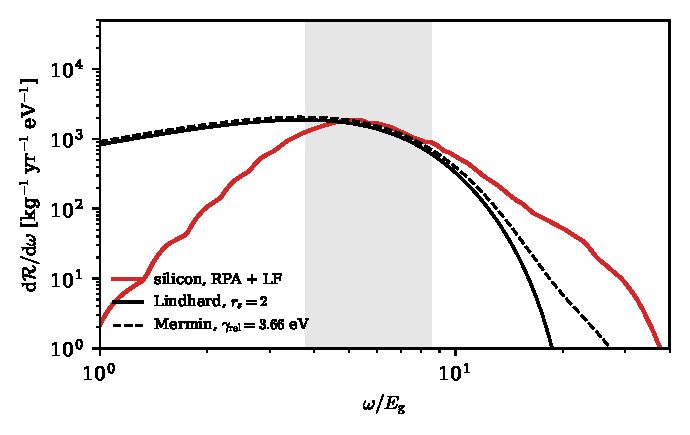
\includegraphics[width=0.82\linewidth]{figures/ch10/limit10_3a.pdf}
\captionof{figure}{Spectrum of silicon at $\mchi = \SI{100}{MeV}$, heavy mediator, $\sigmae = \SI{e-37}{cm^2}$, $\rho_\chi = \SI{0.3}{GeV.cm^{-3}}$ and the standard halo, against $\omega/\Eg$ with $\Eg = \SI{1.11}{eV}$, the step-model gap that accompanies the tables. Red: the random-phase loss function of silicon with local fields (the tables of \cref{fig:10-screening}). Black: the Lindhard loss function of the electron gas at the valence density, $r_s = 2$; dashed, the Mermin function with $\gamma_{\mathrm{rel}} = \SI{3.66}{eV}$, a fit parameter. All three are integrated over the same momenta, from 0.49 to \SI{22.5}{keV}. Gray: from the upper absorption peak of silicon, \SI{4.2}{eV}, to $k_{\mathrm{F}}v_{\mathrm{max}} = \SI{9.5}{eV}$, a band chosen for this figure. There the Lindhard spectrum is between 0.70 and 1.48 times the crystal one.}\label{fig:10-gas-limit}
\par}
\smallskip
Below the band the gas has no gap and overestimates the rate, by 24 at \SI{2}{eV}; above it the gas has no electrons faster than $v_{\mathrm{F}}$ and loses the high-energy tail, and the integrated agreement at this mass comes from the two errors cancelling.
\end{limitbox}

\subsection{Plasmon pole and residue}\label{sec:10.3-pole}

Below $q_{\mathrm{c}}$ the loss function of the gas is the particle--hole continuum plus a line, \cref{eq:4.5-plasmonL}, whose weight is $\pi$ divided by the slope of $\varepsilon_1$ at the zero. At small $q$ the slope follows from the high-frequency expansion of \cref{sec:4.5} kept to order $q^2$~\cite[Eq.~(5)]{kozaczuk2020plasmon},
\begin{equation*}
  \varepsilon_1(q,\omega) \simeq 1 - \frac{\omega_p^2}{\omega^2}\Bigl(1 + \frac{3}{5}\,\frac{q^2v_{\mathrm{F}}^2}{\omega^2}\Bigr) .
\end{equation*}
Its zero is $\omega_{\mathrm{pl}}^2 = \omega_p^2 + \tfrac35q^2v_{\mathrm{F}}^2$, the first two terms of \cref{eq:4.5-dispersion}. With $x = \tfrac35q^2v_{\mathrm{F}}^2/\omega_{\mathrm{pl}}^2$ the zero condition reads $\omega_p^2(1 + x) = \omega_{\mathrm{pl}}^2$, and differentiating,
\begin{gather*}
  \frac{\partial\varepsilon_1}{\partial\omega}\bigg|_{\omega_{\mathrm{pl}}} = \frac{2\omega_p^2}{\omega_{\mathrm{pl}}^3}\,(1 + 2x) = \frac{2}{\omega_{\mathrm{pl}}}\,\frac{1 + 2x}{1 + x} , \\
  \frac{\pi}{\partial\varepsilon_1/\partial\omega} = \frac{\pi\omega_{\mathrm{pl}}}{2}\,Z_L(q) , \qquad Z_L(q) = \frac{1 + x}{1 + 2x} = 1 - \frac35\,\frac{q^2v_{\mathrm{F}}^2}{\omega_p^2} + O(q^4) .
\end{gather*}
The factor $Z_L$ is the residue of the longitudinal photon propagator at the plasmon pole that Kozaczuk and Lin use for the plasmon's polarization vector~\cite[Eq.~(7)]{kozaczuk2020plasmon}; here it is the weight of the line in $L$. The first moment of the line, $\omega_{\mathrm{pl}}\cdot(\pi\omega_{\mathrm{pl}}/2)Z_L = (\pi/2)\omega_p^2(1 + x)(1 - x)$, is the whole $f$-sum to order $q^2$: at small $q$ the plasmon carries all of the oscillator strength, and the continuum none. Integrating \cref{eq:10.2-rate} over the delta function gives
\begin{keyresult}[Plasmon production rate]
\begin{equation}
  \mathcal{R}_{\mathrm{pl}} = \frac{\rho_\chi\,\sigmae}{8\pi^2\alpha\,\rho_T\,\mchi\,\mu_{\chi e}^2}\int_0^{q_{\mathrm{c}}}\dd q\;q^3\,\FDM(q)^2\,\eta\bigl(\vmin(q,\omega_{\mathrm{pl}}(q))\bigr)\,\frac{\pi\omega_{\mathrm{pl}}(q)}{2}\,Z_L(q) ,
  \label{eq:10.3-plrate}
\end{equation}
with $\vmin$ of \cref{eq:1.3-vmin}, the splitting $\Delta_\chi$ included. Beyond the small-$q$ forms, $\omega_{\mathrm{pl}}$ is the exact zero of $\varepsilon_1$ and $(\pi\omega_{\mathrm{pl}}/2)Z_L$ is replaced by $\pi/(\partial\varepsilon_1/\partial\omega)$ there.
\end{keyresult}
\noindent The small-$q$ residue, with $Z_L$ expanded to $1 - \tfrac35q^2v_{\mathrm{F}}^2/\omega_p^2$ as in the limit check below, agrees with the exact one of the Lindhard function to $10^{-4}$ at $q = 0.1\,k_{\mathrm{F}}$ and $8\times10^{-3}$ at $0.3\,k_{\mathrm{F}}$, the size of the dropped $q^4$ terms. Near the cutoff the two part. The exact line carries 0.99 of the $f$-sum at $q_{\mathrm{c}}/2$, 0.77 at $0.9\,q_{\mathrm{c}}$, and nothing at $q_{\mathrm{c}}$. At the continuum edge $\omega_+$ the real part of the Lindhard function contains $(1 - \nu_-^2)\ln|(\nu_- + 1)/(\nu_- - 1)|$ with $\nu_- \to 1$ (\cref{eq:4.5-lindhard}), and its derivative in $\omega$ diverges logarithmically. The slope at the zero therefore grows without bound, and the weight of the line goes to zero as the line touches the continuum. The weight it loses appears in the continuum just below it; this is Landau damping seen in the residue.

The cutoff itself depends on how the dispersion is treated, and the literature uses several values. The exact zero of $\varepsilon_{\mathrm{Lin}}$ meets the edge $\omega_+ = qv_{\mathrm{F}} + q^2/2m_e$ at $q_{\mathrm{c}} = \SI{2.60}{keV}$ and \SI{24.8}{eV} (\cref{sec:4.5}). The quadratic dispersion, with the $q^4$ terms dropped, meets it at \SI{2.24}{keV} and \SI{20.6}{eV}, a dispersion fixed at $\omega_p$ at \SI{1.88}{keV}, and the estimate $\omega_p/v_{\mathrm{F}}$ is \SI{2.38}{keV}. The spread is large because the correction is not small near the cutoff: at \SI{2.24}{keV}, $\tfrac35q^2v_{\mathrm{F}}^2/\omega_p^2 = 0.53$. All four values lie close to the zone scale $2\pi/a = \SI{2.28}{keV}$ of silicon. The crystal shows the same onset (\cref{fig:10-plasmon}). In the silicon tables the loss peak follows the gas dispersion from \SI{18.9}{eV} at \SI{0.5}{keV} to \SI{22.3}{eV} at \SI{2.45}{keV}, with a half-maximum width of about \SI{5}{eV}. Beyond that it broadens fast: at \SI{3.5}{keV} the half maximum spans 17.7 to \SI{32.2}{eV}, and at \SI{4.6}{keV} 14.9 to \SI{44}{eV}. The tables place the small-$q$ peak \SI{2.5}{eV} above the measured \SI{16.4}{eV}, because the scissor that fixes the gap also raises the interband energies that push the plasmon up (\cref{we:4-siplasmon}).

Kurinsky, Baxter, Kahn and Krnjaic wrote the plasmon rate of a fast component of dark matter with a light mediator as the optical line shape times a logarithm~\cite[Eqs.~(13) and (14)]{kurinsky2020dark}. It follows from \cref{eq:10.2-rate} in two steps. A light mediator has $\FDM = (q_0/q)^2$, so $q^3\FDM^2 = q_0^4/q$. Replacing $L(q,\omega)$ by its optical value $L(0,\omega)$ for all $q$ below a cutoff then gives
\begin{equation*}
  \frac{\dd\mathcal{R}}{\dd\omega} = \frac{\rho_\chi\,\sigmae\,q_0^4}{8\pi^2\alpha\,\rho_T\,\mchi\,\mu_{\chi e}^2}\;L(0,\omega)\int_0^{q_{\mathrm{c}}}\frac{\dd q}{q}\;\eta\bigl(\vmin(q,\omega)\bigr) ,
\end{equation*}
which is Ref.~\cite[Eq.~(14)]{kurinsky2020dark} in the book's normalization. They set the cutoff at $2\pi/a \sim \SI{5}{keV}$ with $a$ the lattice spacing~\cite[Eq.~(4)]{kurinsky2020dark}. For silicon, with $a = \SI{5.43}{\angstrom}$, $2\pi/a$ is \SI{2.28}{keV}; \SI{5}{keV} corresponds to a length of \SI{2.5}{\angstrom}, close to the bond length. The error this makes is logarithmic, because the integrand is $1/q$. For a particle of speed $v = 0.1$ the plasmon opens at $q_{\mathrm{min}} = \omega_p/v = \SI{0.17}{keV}$, and moving the cutoff from $q_{\mathrm{c}} = \SI{2.60}{keV}$ to \SI{5}{keV} raises the integral by $\ln(5/0.166)/\ln(2.60/0.166) = 1.24$, or 1.31 from \SI{2.24}{keV}. A measure growing like $q$ would have given $(5/2.60)^2 = 3.7$. The constant optical line shape also ignores the weight the line loses near $q_{\mathrm{c}}$, which removes a further 3 percent of the logarithmic integral. For a fast component the choice of cutoff therefore moves the optical form by 25 to 30 percent, not by a factor of several.

\begin{limitbox}[Plasmon production from the pole of $1/\varepsilon$][lim:10.3b]
Below the cutoff the plasmon is the line $L \simeq (\pi\omega_{\mathrm{pl}}/2)Z_L\,\delta(\omega - \omega_{\mathrm{pl}}(q))$, with $\omega_{\mathrm{pl}}^2 \simeq \omega_p^2 + \tfrac35q^2v_{\mathrm{F}}^2$ and $Z_L \simeq 1 - \tfrac35q^2v_{\mathrm{F}}^2/\omega_p^2$~\cite[Eqs.~(5) and (7)]{kozaczuk2020plasmon}. Kurinsky et al. write the light-mediator rate with $L$ taken at $q = 0$ up to the cutoff~\cite[Eqs.~(4), (13) and (14)]{kurinsky2020dark}.
\par\smallskip
{\centering
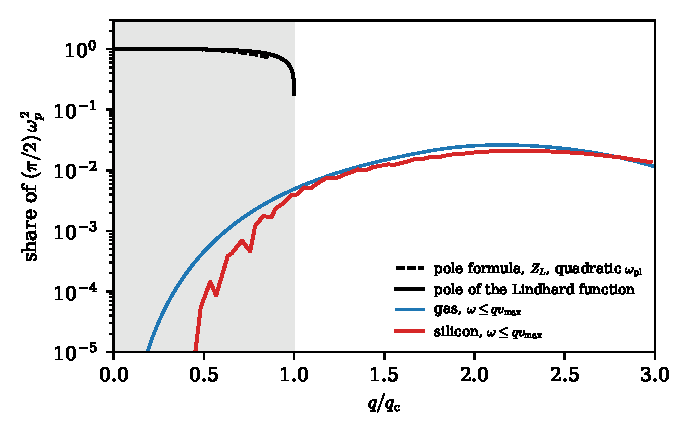
\includegraphics[width=0.82\linewidth]{figures/ch10/limit10_3b.pdf}
\captionof{figure}{Share of the valence $f$-sum $(\pi/2)\omega_p^2$ of silicon, $\omega_p = \SI{16.6}{eV}$, against $q/q_{\mathrm{c}}$ with $q_{\mathrm{c}} = \SI{2.60}{keV}$. Dashed: the first moment of the pole formula, $\omega_{\mathrm{pl}}^2Z_L/\omega_p^2$ with the quadratic dispersion, up to its own cutoff at \SI{2.24}{keV}; dotted: the optical line shape continued to \SI{5}{keV}. Solid black: the pole of the Lindhard function at $r_s = 2$, whose weight falls to zero at $q_{\mathrm{c}}$. Blue: the weight of the Lindhard continuum below $\omega = qv_{\mathrm{max}}$, the most a halo particle can deposit; red: the same for the random-phase loss function of silicon with local fields, from \SI{0.49}{keV}. Gray: $q < q_{\mathrm{c}}$, where the pole exists.}\label{fig:10-pole-limit}
\par}
\smallskip
Near $q_{\mathrm{c}}$ the small-$q$ residue misstates the line, whose weight goes to zero at the continuum edge, and beyond $q_{\mathrm{c}}$ there is no line at all. The weight within reach of the halo is never more than about 3 percent of the $f$-sum and lies in the pair continuum.
\end{limitbox}

\subsection{Plasmon threshold speed}\label{sec:10.3-reach}

A particle of speed $v$ makes a plasmon of momentum $q$ only if $v \ge \vmin(q,\omega_{\mathrm{pl}}(q)) = \omega_{\mathrm{pl}}(q)/q + q/2\mchi$ for elastic scattering, and \cref{eq:10.3-plrate} is nonzero only if this holds for some $q < q_{\mathrm{c}}$. The phase velocity $\omega_{\mathrm{pl}}/q$ is infinite at $q \to 0$ and falls as $q$ grows. At $q_{\mathrm{c}}$ the line meets the continuum edge, where $\omega_{\mathrm{pl}} = \omega_+$ and $\omega_+/q = v_{\mathrm{F}} + q/2m_e$, which rises with $q$; in the Lindhard function the phase velocity reaches its smallest value at $0.989\,q_{\mathrm{c}}$, within $10^{-3}$ of its value at $q_{\mathrm{c}}$. For a heavy particle the slowest one that can make a plasmon therefore moves at
\begin{equation}
  v_{\mathrm{th}} \simeq \frac{\omega_+(q_{\mathrm{c}})}{q_{\mathrm{c}}} = v_{\mathrm{F}} + \frac{q_{\mathrm{c}}}{2m_e} ,
  \label{eq:10.3-vth}
\end{equation}
plus $q_{\mathrm{c}}/2\mchi$ for a finite mass. The threshold is set by the electrons, not by the dark matter. The plasmon is undamped only while its phase velocity exceeds $\omega_+/q$, the largest ratio of energy to momentum that a single pair can have, so the slowest plasmon is as fast as the fastest pair. At the silicon valence density $v_{\mathrm{th}} = 9.54\times10^{-3}$, or \SI{2860}{km.s^{-1}}, and with the quadratic dispersion and its cutoff at \SI{2.24}{keV}, $9.18\times10^{-3}$ or \SI{2750}{km.s^{-1}}. Either is 3.5 to 3.6 times the largest speed of the halo, $v_{\mathrm{max}} = \SI{794.5}{km.s^{-1}}$ (\cref{eq:1.2-vmax}), and agrees with the estimate $v \gtrsim 10^{-2}$ of Kurinsky et al.~\cite[Eq.~(7)]{kurinsky2020dark}. \Cref{we:4-siplasmon} reached the same conclusion from the other side: the line $\omega = qv_{\mathrm{max}}$ reaches $\omega_p$ only at $q = \SI{6.27}{keV}$, more than twice $q_{\mathrm{c}}$.

\begin{figure}[tbp]
  \centering
  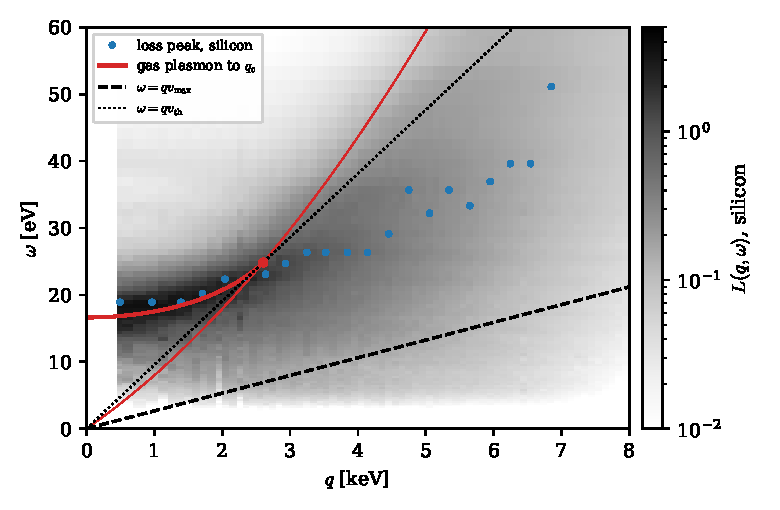
\includegraphics[width=0.9\linewidth]{figures/ch10/fig10_3.pdf}
  \caption{The silicon plasmon against the reach of halo dark matter. Gray scale: the random-phase loss function of silicon with local fields, $L(q,\omega)$, from the tables of Knapen, Kozaczuk and Lin~\cite{knapen2021dark}, averaged over the directions of $\vect{q}$ in bins of \SI{100}{eV} in $|\vect{q}|$ starting at \SI{0.49}{keV}, logarithmic scale. Blue dots: the maximum of $L$ in every third bin. Red: the undamped plasmon of the electron gas at the valence density, the exact zero of $\varepsilon_{\mathrm{Lin}}$, up to $q_{\mathrm{c}} = \SI{2.60}{keV}$ (dot), and the continuum edge $\omega_+ = qv_{\mathrm{F}} + q^2/2m_e$ (thin). Dashed: $\omega = qv_{\mathrm{max}}$, the largest energy a halo particle deposits at momentum $q$. Dotted: $\omega = qv_{\mathrm{th}}$ with $v_{\mathrm{th}} = 9.54\times10^{-3}$ of \cref{eq:10.3-vth}, the slowest particle that reaches the plasmon of the gas. The tables place the small-$q$ loss peak at \SI{18.9}{eV}, against the measured \SI{16.4}{eV}, because of the scissor shift that fixes their gap.}
  \label{fig:10-plasmon}
\end{figure}

In the standard halo the speed distribution ends at $v_{\mathrm{max}}$, and $\mathcal{R}_{\mathrm{pl}}$ is zero at every mass. The suppression is not a power of a small ratio. Remove the escape cut and keep the Maxwellian tail of \cref{sec:1.2}: the fraction of particles faster than \SI{2750}{km.s^{-1}} in the laboratory is about $10^{-49}$, and about $10^{-53}$ above \SI{2860}{km.s^{-1}}. A real halo is not Maxwellian that far out, and these numbers only measure how far the plasmon lies from the bulk of the distribution, 10.5 to 11 times $v_0$ beyond the speed of the Earth.

\begin{workedexample}{The plasmon rate of silicon at the highest halo speed}\label{we:10-plasmon}
Take a particle at $v = v_{\mathrm{max}} = 2.650\times10^{-3}$, heavy enough that $q/2\mchi$ is negligible; at \SI{100}{MeV} it raises $v_{\mathrm{th}}$ by 0.14 percent. At momentum $q$ it deposits at most $qv_{\mathrm{max}}$: \SI{5.94}{eV} at the quadratic cutoff \SI{2.24}{keV}, \SI{6.90}{eV} at $q_{\mathrm{c}} = \SI{2.60}{keV}$. The plasmon of the gas sits at 20.6 and \SI{24.8}{eV} there. The distance between the plasmon and the reach, $\omega_{\mathrm{pl}}(q) - qv_{\mathrm{max}}$, is smallest at $q = \SI{1.34}{keV}$, where it is \SI{14.7}{eV} for the exact zero of the Lindhard function (the quadratic dispersion gives \SI{14.5}{eV} at \SI{1.72}{keV}). The particle is short of the plasmon by about $\omega_p$, at every momentum where the plasmon exists, and \cref{eq:10.3-plrate} gives $\mathcal{R}_{\mathrm{pl}} = 0$.

The silicon plasmon is not a sharp line: interband pairs give it a width of \SI{3.7}{eV} already at $q \to 0$ (\cref{we:4-siplasmon}). The tables show what the particle meets instead. In the bin at \SI{2.28}{keV} the loss peak sits at \SI{22.3}{eV}, and at the reach of the particle, \SI{6.0}{eV}, $L$ is 6.9 percent of its peak value; the energies the particle can deposit hold $1.7\times10^{-3}$ of the valence $f$-sum. At \SI{2.57}{keV} the numbers are 8.5 percent and $4.0\times10^{-3}$. These are pairs on the low-energy side of the resonance, the same pairs that the rate of \cref{sec:10.2} already counts. They also carry little of that rate. At \SI{100}{MeV}, momenta below \SI{2.60}{keV} give $4.9\times10^{-4}$ of the heavy-mediator rate (\num{9.6e-5} below \SI{2.24}{keV}) and 2.5 percent of the light-mediator rate.

The answer is that the plasmon rate of silicon is zero for halo dark matter, not small: the pole needs \SI{2750}{km.s^{-1}} or more, and the halo stops at \SI{794.5}{km.s^{-1}}. A loss-function rate that seems to contain ``plasmon'' events at 15 to \SI{25}{eV} draws them from $q > \SI{5.7}{keV}$, where \cref{fig:10-plasmon} shows only the broad pair continuum.
\end{workedexample}

The pole opens for a fast component of dark matter, for an exothermic splitting, or when a third body takes the momentum, and each case belongs to another section. A fast component, accelerated or boosted, can exceed $v_{\mathrm{th}}$, and \cref{eq:10.3-plrate} applies with its speed distribution in $\eta$ (\cref{sec:10.9}). An exothermic transition lowers $\vmin$ through $\Delta_\chi < 0$ in \cref{eq:1.3-vmin}, and a particle at $v_{\mathrm{max}}$ reaches the line once $|\Delta_\chi| \gtrsim \SI{14.7}{eV}$, the closest approach of the worked example; \cref{sec:17.3} treats such down-scattering into collective modes. When the dark matter scatters off a nucleus, the recoiling ion can emit a plasmon whose momentum is small, as in bremsstrahlung. Kozaczuk and Lin computed this rate in the electron-gas picture and found it four to five orders of magnitude below the elastic nuclear rate for masses from \SI{10}{MeV} to \SI{1}{GeV}~\cite{kozaczuk2020plasmon}; it is a process of the joint electron--lattice response of \cref{chap:12}.

\subsection{Plasmon decay into pairs and phonons}\label{sec:10.3-decay}

With the nuclei clamped, a plasmon of silicon decays into electron--hole pairs and nothing else. At the measured loss peak, \SI{16.4}{eV}, vertical interband transitions are open, $\varepsilon_2 = 0.22$ where $\varepsilon_1$ vanishes, and the width of the loss peak follows from that value (\cref{we:4-siplasmon}). The branching ratio into pairs is one, and \cref{sec:8.7} showed that the screened pair weights of \cref{eq:8.7-screened} already contain the plasmon peak, so that a plasmon is not a separate final state of silicon. Its energy is shared by the pairs, and the step model \cref{eq:1.5-step} turns \SI{16.4}{eV} into five; the cascade that produces them is the subject of \cref{sec:18.1}.

With the lattice free to move, part of the decay goes into pairs plus phonons. By the decomposition theorem \cref{eq:8.6-decomp}, the absorptive part of the response at $(\vect{q},\omega_{\mathrm{pl}})$ splits into a zero-phonon sector $S^0$ and a phonon-dressed sector $S^+$. Since $L = \varepsilon_2/|\varepsilon|^2$ and the factor $|\varepsilon|^2$ is common to both sectors, the phonon branching of the plasmon is
\begin{equation}
  B_{\mathrm{pl}}^+(\vect{q}) = \frac{S^+(\vect{q},\omega_{\mathrm{pl}})}{S^0(\vect{q},\omega_{\mathrm{pl}}) + S^+(\vect{q},\omega_{\mathrm{pl}})} = \frac{\varepsilon_2^+(\vect{q},\omega_{\mathrm{pl}})}{\varepsilon_2(\vect{q},\omega_{\mathrm{pl}})} ,
  \label{eq:10.3-branch}
\end{equation}
the share of phonon-assisted absorption in $\varepsilon_2$ at the plasmon energy. At \SI{16}{eV} direct transitions are allowed. A phonon-assisted transition needs one electron--phonon vertex besides the density vertex, and its amplitude carries the vertex over an energy denominator. With optical-phonon vertices of a few tenths of an eV and denominators of a few eV, \cref{sec:6.5} found the phonon-assisted absorption to be about $10^{-2}$ of the direct one per coupled mode. At the plasmon energy the direct transitions are strong, and the same estimate puts $B_{\mathrm{pl}}^+$ between $10^{-3}$ and $10^{-2}$; it has not been computed. The phonons counted by \cref{eq:10.3-branch} always come with a pair. A decay into phonons alone would have to pass \SI{16}{eV} to modes of at most \SI{64}{meV}, some 260 of them, with no electronic final state, and it is not part of this estimate. Kurinsky et al. needed plasmons that decay mostly into phonons to explain low-energy excess events~\cite{kurinsky2020dark}; the estimate here gives a phonon share of at most a percent.

\Cref{sec:10.4} turns from the number of the electrons to their spin and their current.

\section{Spin and current couplings}\label{sec:10.4}

Dark matter with an anapole moment couples to electrons partly through $\mathcal{O}_8 = \vect{S}_\chi\cdot\vect{v}^\perp$, the dark-matter spin times the relative velocity of the two particles (\cref{sec:8.1}). For an electron at rest the relative velocity equals the velocity of the dark matter, typically $10^{-3}$, and the rate is the density rate of \cref{sec:10.2} times $|\bar{\vect{v}}_{\mathrm{T}}|^2/4$, with $\bar{\vect{v}}_{\mathrm{T}}$ the part of the dark matter's mean velocity across $\vect{q}$. The valence electrons of silicon, however, are not at rest. Taken as a free gas at their density they move at $v_{\mathrm{F}} = 7.0\times10^{-3}$, nine times the dispersion $v_0$ of the halo, and the velocity in $\mathcal{O}_8$ is the difference between the dark-matter velocity and the electron velocity. The electron's own motion couples through the electron current, a separate row of the response matrix, which the medium screens differently from the density. Every coupling beyond the density needs new responses of the crystal, each screened in its own way, and an interference term between rows; the interference term has not been computed.

\subsection{The minimal response table}\label{sec:10.4-table}

The rows of \cref{eq:8.1-rows} for the electrons are the density $n_e$, the spin density $\vect{s}_e$, the current $\vect{j}_e$, the spin current $\mathcal{J}^{\alpha\beta}_e$ and the kinetic-energy density $\mathcal{T}_e$, three of them vectors and one a tensor. Counted by components they are 17 operators, and the response matrix has 289 elements at every $(\vect{q},\omega)$. Three constraints reduce them to a few functions: charge conservation, spin-rotation symmetry and the combined symmetry of inversion and time reversal. \Cref{app:D.30} derives each step.

Charge conservation comes first. For a Hamiltonian with local potentials the current along $\vect{q}$, $j_{\mathrm{L}} = \hat{\vect{q}}\cdot\vect{j}_e$, has the matrix elements of $(\omega/q)\,n_e$ between eigenstates (\cref{eq:4.3-continuity}), and every element of the response matrix that contains $j_{\mathrm{L}}$ is a multiple of one that does not (\cref{eq:D.30-continuity}). On the dark-matter side the same holds for the velocity, $\hat{\vect{q}}\cdot\bar{\vect{v}}_\chi = (\omega + \Delta_\chi)/q$. For elastic dark matter the two longitudinal parts cancel (\cref{eq:8.1-transverse}), and only the transverse current survives, $j_{\mathrm{T}i} = \hat{\vect{e}}_i\cdot\vect{j}_e$ along two unit vectors $\hat{\vect{e}}_{1,2}$ perpendicular to $\vect{q}$. If the electron spin is conserved, the spin current obeys its own continuity equation, and only its transverse velocity components $\mathcal{J}^{\mathrm{T}i,\beta}_e = \hat e^\alpha_i\mathcal{J}^{\alpha\beta}_e$ survive.

Without spin--orbit coupling and without magnetic order the Hamiltonian is unchanged by a rotation of all spins, and the ground state of silicon is a spin singlet. The density, the current and the kinetic-energy density do not act on spin and make singlet pairs; the spin density and the spin current make triplets. Singlet and triplet pairs never interfere, and the response matrix splits into a singlet block on $\{n_e, j_{\mathrm{T}1}, j_{\mathrm{T}2}, \mathcal{T}_e\}$ and a triplet block on $\{s^z_e, \mathcal{J}^{\mathrm{T}1,z}_e, \mathcal{J}^{\mathrm{T}2,z}_e\}$, the same for every spin component. For independent electrons the triplet block is a quarter of the singlet one (\cref{eq:D.30-quarter}): the spin vertex $\sigma^z/2$ has $(\pm\frac12)^2 = \frac14$ where the density vertex has 1, and the spatial sums are the same. The unscreened crystal form factor of \cref{sec:10.1} therefore also gives the spin-dependent rate of $\mathcal{O}_4$ at the independent-particle level, up to the spin traces of the two particles. Beyond independent particles the factor $\frac14$ fails, as the next subsection shows.

Silicon and germanium are also symmetric under inversion combined with time reversal, which makes every element of both blocks real. The singlet block on $\{n_e, j_{\mathrm{T}1}, j_{\mathrm{T}2}\}$ is then a real symmetric $3\times3$ matrix: six real functions of $(\vect{q},\omega)$, namely $S_{nn}$, two density--current elements and three current--current elements. A complete table holds them twice, screened and for independent particles, and the independent-particle set fixes the triplet block at that level. The table then holds twelve functions. Operator $\mathcal{O}_2$ alone needs more: its velocity squared brings in $\mathcal{T}_e$, with four further elements in each version. For $\vect{q}$ along a two-, three- or fourfold axis of the cubic crystal, a rotation about $\hat{\vect{q}}$ leaves the density unchanged and turns the transverse current, so the density--current elements vanish.

\Cref{tab:10-minimal} sorts the operators of \cref{tab:8-operators} by block.

\begin{table}[tbp]
  \caption{The minimal response table: the rows of the electronic response matrix that each non-relativistic operator of \cref{tab:8-operators} needs, and their screening. The longitudinal current and spin current have been eliminated by continuity (elastic scattering, local potentials, electron spin conserved). Screening is for a cubic crystal without spin--orbit coupling or magnetic order. Singlet rows make spin-singlet electron--hole pairs and triplet rows spin-triplet pairs; the two blocks do not interfere. Notation: $j_{\mathrm{T}}$, current across $\vect{q}$; $\mathcal{J}_{\mathrm{T}}$: spin current with its velocity index across $\vect{q}$. With inversion and time reversal, the singlet block on $\{n_e, j_{\mathrm{T}1}, j_{\mathrm{T}2}\}$ holds six real functions per $(\vect{q},\omega)$. For independent particles the triplet block is one quarter of the singlet block (\cref{eq:D.30-quarter}).}
  \label{tab:10-minimal}
  \centering\small
  \renewcommand{\arraystretch}{1.25}
  \begin{tabular}{@{}>{\raggedright\arraybackslash}p{0.2\linewidth}>{\raggedright\arraybackslash}p{0.21\linewidth}>{\raggedright\arraybackslash}p{0.13\linewidth}>{\raggedright\arraybackslash}p{0.37\linewidth}@{}}
    \toprule
    Operators & Rows & Block & Screening \\
    \midrule
    $\mathcal{O}_1$, $\mathcal{O}_{11}$ & $n_e$ & singlet & head and local fields (\cref{sec:10.2}) \\
    $\mathcal{O}_5$, $\mathcal{O}_8$ & $n_e$, $j_{\mathrm{T}}$ & singlet & $n_e$ as above; $j_{\mathrm{T}}$ unscreened at the head on symmetry axes, local fields only (about \SI{10}{\percent}) \\
    $\mathcal{O}_2$ & $n_e$, $j_{\mathrm{T}}$, $\mathcal{T}_e$ & singlet & $n_e$, $j_{\mathrm{T}}$ as above; $\mathcal{T}_e$ at the head and through local fields \\
    $\mathcal{O}_4$, $\mathcal{O}_6$, $\mathcal{O}_9$, $\mathcal{O}_{10}$ & $\vect{s}_e$ & triplet & none; electron--hole attraction beyond independent particles \\
    $\mathcal{O}_3$, $\mathcal{O}_7$, $\mathcal{O}_{12}$--$\mathcal{O}_{15}$ & $\vect{s}_e$, $\mathcal{J}_{\mathrm{T}}$ & triplet & none; as above \\
    \bottomrule
  \end{tabular}
\end{table}

The current and spin-current rows are computed from the same Kohn--Sham states as the density, with one extra step: a nonlocal pseudopotential adds a commutator to the current vertex (\cref{eq:E.7-vNL}), and leaving the commutator out changes the transverse current of silicon by about \SI{10}{\percent}.

\subsection{Screening of non-density rows}\label{sec:10.4-screening}

A row is screened to the extent that it correlates with the charge (\cref{sec:8.4}). In the reciprocal-lattice basis of \cref{sec:4.6} the rule takes the form of \cref{eq:D.30-dyson}. The Coulomb interaction acts on the densities $n_e(\vect{q} + \vect{G})$, and any other row enters as an external vertex. Its screened response differs from the proper one by a term built from its proper correlation with those densities.

The density is screened at the head and through local fields (\cref{sec:10.2}). The longitudinal current is screened exactly as the density, since it is the density times $\omega/q$.

The transverse current cannot drive the long-wavelength density when $\hat{\vect{q}}$ lies on a symmetry axis: the rotation that leaves $\vect{q}$ fixed turns $j_{\mathrm{T}}$ and leaves $n_e(\vect{q})$ alone, so their correlation at $\vect{G} = 0$ vanishes. The head dominates the screening of the density at small $q$, but for $j_{\mathrm{T}}$ it then drops out, and the transverse current feels only the local fields, through its correlation with $n_e(\vect{q} + \vect{G})$ at $\vect{G} \neq 0$. Off the axes the head returns through the mixing of longitudinal and transverse components, but weakly. In the empirical-pseudopotential model of silicon of \cref{fig:10-fcrys-limit}, with $\vect{q}$ along the generic direction $(5,3,1)$, the head changes $\Tr S_{\vect{j}_{\mathrm{T}}\vect{j}_{\mathrm{T}}}$ by less than $10^{-3}$ at $q_0$ and \SI{5}{eV}, while it lowers $S_{nn}$ by a factor 3.9. With local fields the current response falls by \SI{15}{\percent} at $q_0$ and \SI{5}{eV}, by 11 at \SI{10}{eV}, and by 8 to \SI{9}{\percent} at $2q_0$; along $[100]$ at $q_0$ and \SI{5}{eV} it falls by \SI{4}{\percent}. The density response at the same point falls to 0.22 of its independent-particle value.

The kinetic-energy density is a scalar under the point group, like the density itself, and correlates with the charge already at $\vect{G} = 0$. It is screened at the head. The same correlation gives the absorption of a scalar its photon-reducible part (\cref{sec:8.4-mixing}), which \cref{sec:10.7} computes.

The spin density and the spin current are unscreened. The Coulomb interaction acts on the total density of both spins and not on their difference, so a triplet row has no proper correlation with the charge, and \cref{eq:D.30-dyson} leaves it as it is. Beyond independent particles, the triplet rows feel the attraction between the electron and the hole. In the language of \cref{sec:4.9} the triplet pair keeps the direct kernel and loses the exchange kernel, the part that carries the local fields. \Cref{sec:10.5-triplet} computes the effect of the direct kernel on the triplet rows. Spin--orbit coupling mixes the two blocks, by amounts that \cref{sec:10.6} estimates near the band edges.

The difference between the screening of the current row and the screening of the density row takes a simple form at long wavelength. There the transverse current response is fixed by the transverse dielectric function and the density response by the loss function (\cref{eq:D.30-optical}),
\begin{equation}
  \frac{\Tr S_{\vect{j}_{\mathrm{T}}\vect{j}_{\mathrm{T}}}(\vect{q},\omega)}{S_{nn}(\vect{q},\omega)} \;\to\; \frac{2\omega^2}{q^2}\,|\varepsilon(\omega)|^2 \qquad (q \to 0) ,
  \label{eq:10.4-optical}
\end{equation}
and for independent particles the same ratio is $2\omega^2/q^2$ without the factor $|\varepsilon|^2$. At \SI{3}{eV} silicon has $|\varepsilon|^2 = 761$ (\cref{sec:10.7-darkphoton}). At small momentum transfer the medium raises the weight of the current row against the density row by orders of magnitude. At keV momenta the head screening weakens, to a factor 4.2 at $q_0$ and 1.2 at \SI{8}{keV} for the density row (\cref{sec:10.2-corrections}), and the enhancement of the current row weakens with it.

For independent particles the spin-current block of $\mathcal{O}_3$, $\mathcal{O}_7$ and $\mathcal{O}_{12}$--$\mathcal{O}_{15}$ is a quarter of the current block, as the spin block is of the density block.

The sum-rule bounds of \cref{sec:10.2} do not carry over to rows other than the density as they stand~\cite[Eqs.~(4.16)--(4.21)]{catena2025general}. The rate of a non-density coupling can contain combinations of responses that need not be positive at each energy, and the current--current combination of anapole dark matter at \SI{15}{keV} in silicon is negative at every energy. And the Coulomb kernel bounds the static step of the density by one but does not limit the static value of an unscreened row; for the spin coupling the static value exceeds one by a factor of about 20 at \SI{500}{eV}. The structure of \cref{tab:10-minimal} avoids the negative combinations and the unbounded static values: each diagonal block obeys its own sum rules, and the cross terms are bounded by positivity, as the next subsection shows.

\begin{limitbox}[Crystal responses of the effective operators][lim:10.4a]
For $\mathcal{O}_8 = \vect{S}_\chi\cdot\vect{v}^\perp$ with the electron at rest, the rate per unit volume of momentum transfer is the rate of the density coupling, screened through the loss function, times $|\bar{\vect{v}}_{\mathrm{T}}|^2/4$: $\dd\varGamma_8/\dd^3q = (|\bar{\vect{v}}_{\mathrm{T}}|^2/4)\,\dd\varGamma_1/\dd^3q$~\cite[Eq.~(6)]{hochberg2025determining}. The crystal responses of Refs.~\cite{catena2021crystal,trickle2023exceed} keep the current row, without its screening.
\par\smallskip
{\centering
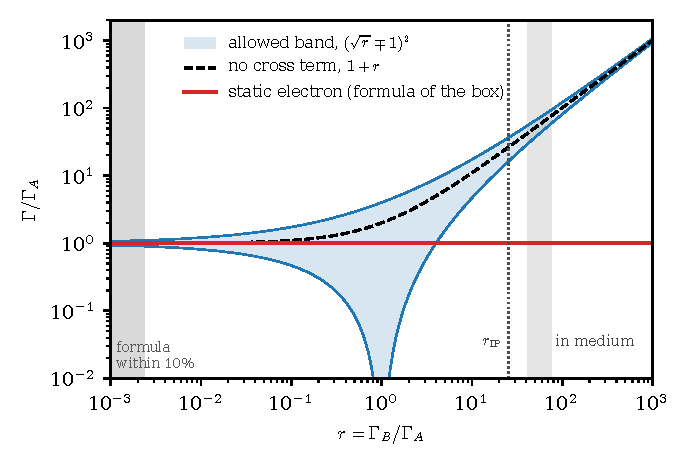
\includegraphics[width=0.82\linewidth]{figures/ch10/limit10_4a.pdf}
\captionof{figure}{Rate of $\mathcal{O}_8 = \vect{S}_\chi\cdot\vect{v}^\perp$ (spin-$\frac12$ dark matter, heavy mediator, elastic) relative to the static-electron formula of the box, $\varGamma_A$, against the ratio $r = \varGamma_B/\varGamma_A$ of the current-row rate $\varGamma_B$ to the formula. Blue: the band that positivity allows when the density--current cross term is not computed, $(\sqrt r \mp 1)^2$ (\cref{eq:10.4-band}). Dashed: $1 + r$, exact for responses averaged over the directions of $\vect{q}$, for which the cross term vanishes. Red: the formula. Gray at left: $r \le 2.4\times10^{-3}$, where every value in the band lies within \SI{10}{\percent} of the formula, $(\sqrt r + 1)^2 \le 1.1$. Dotted: silicon at $\mchi = \SI{10}{MeV}$ for independent particles, $r_{\mathrm{IP}} = 25.3$, from the empirical pseudopotential of Cohen and Bergstresser (model gap \SI{0.82}{eV}, $10^3$ $\vect{k}$ points, 36 conduction bands, bins of \SI{0.1}{eV}, 26-point average over directions, threshold \SI{1.11}{eV}, standard halo of \cref{sec:1.2}). Gray at right: the same ratio with the density row screened, $r_{\mathrm{IP}}\times2.31\times(1 \pm 0.3)$. The factor 2.31 is the screening of the density rate in the random-phase tables with local fields of \cref{sec:10.2}, and $\pm0.3$ the range allowed for the local-field change of the current row.}\label{fig:10-mixed-limit}
\par}
\smallskip
The formula leaves out the electron's own transverse motion, which in silicon carries about 25 times the rate the formula keeps, so the true rate is at least 16 times the formula for independent particles and at least 29 times with the density row screened.
\end{limitbox}

\subsection{Interference bound on a mixed block}\label{sec:10.4-band}

The rate of $\mathcal{O}_8$ shows how the rows combine. With the potentials of \cref{eq:8.1-O7O8} on the density and the current, the contraction \cref{eq:8.2-rate} has a density term, a current term and their interference. Continuity removes the parts along $\vect{q}$ on both sides (\cref{eq:D.30-O8T}). For elastic dark matter, and with the responses averaged over the directions of $\vect{q}$, the velocity integral is the one of \cref{app:A.8} with one change. The density term carries the dark matter's transverse velocity squared, $|\bar{\vect{v}}_{\mathrm{T}}|^2 = v^2 - \vmin^2$ on the energy shell, and its halo average is the second speed moment $\eta_2(\vmin) = 2\int_{\vmin}^\infty\dd v'\,v'\eta(v')$ in place of $\eta$ (\cref{eq:D.30-kernel}).
\begin{keyresult}[Rate of a velocity coupling]
For $\mathcal{O}_8$ with coefficient $c_8^{(e)}(q)$ and spin-$\frac12$ dark matter, the spectrum per unit target mass is
\begin{equation}
  \frac{\dd\mathcal{R}}{\dd\omega} = \frac{\rho_\chi}{16\pi^2\mchi\rho_T}\int\dd q\;q\,\bigl|c_8^{(e)}(q)\bigr|^2\Bigl[\underbrace{\eta_2(\vmin)\,\bar S_{nn}(q,\omega)}_{\text{electron at rest}} + \underbrace{\eta(\vmin)\,\Tr\bar S_{\vect{j}_{\mathrm{T}}\vect{j}_{\mathrm{T}}}(q,\omega)}_{\text{electron motion}}\Bigr] ,
  \label{eq:10.4-O8}
\end{equation}
with $\bar S$ averaged over the directions of $\vect{q}$, for which the density--current cross term vanishes. The first term is the rate of an electron at rest; the second is the electron's own transverse motion.
\end{keyresult}
\noindent The prefactor follows from \cref{eq:8.2-spectrum} with the kernel $\eta/(2q)$ per unit $\dd^3q/(2\pi)^3$ of \cref{eq:A.8-eta} and the factor $\frac14$ of the spin trace. For $c_8^{(e)} = \tilde V$ and $\Tr\bar S_{\vect{j}_{\mathrm{T}}\vect{j}_{\mathrm{T}}} = 0$, \cref{eq:10.4-O8} is the density rate with $\eta \to \eta_2/4$, the form of the box.

We can estimate the two terms before computing them. On the dark-matter side, the ratio $\eta_2/\eta$ is the mean of $|\bar{\vect{v}}_{\mathrm{T}}|^2$ over the particles fast enough to deposit $\omega$. It is $1.1\times10^{-6}$ at $\vmin = 0$, $1.0\times10^{-6}$ at $10^{-3}$ and $0.7\times10^{-6}$ at $2\times10^{-3}$, and it vanishes at the kinematic edge, where the only particles left move along $\vect{q}$. On the target side, the ratio $\Tr\bar S_{\vect{j}_{\mathrm{T}}\vect{j}_{\mathrm{T}}}/\bar S_{nn}$, integrated over $\omega$, is the mean transverse velocity squared of the electrons that make the pairs. In the empirical-pseudopotential model of silicon it is $3.2\times10^{-5}$ at $q_0$ and $2.1\times10^{-5}$ at $2q_0$, close to the free-gas value $\frac25v_{\mathrm{F}}^2 = 2.0\times10^{-5}$. At small $q$ it grows as $2\langle\omega^2\rangle/q^2$, the independent-particle form of \cref{eq:10.4-optical}: at $0.12\,q_0$ the model gives $4.1\times10^{-4}$ against $2\langle\omega^2\rangle/q^2 = 4.4\times10^{-4}$. We expect the electron term to exceed the dark-matter term by a factor of about 20 to 30, and more near the kinematic edge.

Let $\varGamma_A$ be the rate of the density term and $\varGamma_B$ the rate of the current term. The interference bound of \cref{sec:8.3} then limits the full rate whatever the cross term is.
\begin{keyresult}[Band on a mixed block]
For any target, halo and binning,
\begin{equation}
  \bigl(\sqrt{r} - 1\bigr)^2 \;\le\; \frac{\varGamma}{\varGamma_A} \;\le\; \bigl(\sqrt{r} + 1\bigr)^2 , \qquad r = \frac{\varGamma_B}{\varGamma_A} ,
  \label{eq:10.4-band}
\end{equation}
and with responses averaged over directions $\varGamma = \varGamma_A + \varGamma_B$. For independent particles $r$ is written $r_{\mathrm{IP}}$.
\end{keyresult}
\noindent The ratio of the two rates decides how much the cross term can matter. The half-width of the band relative to $1 + r$ is $2\sqrt r/(1 + r)$, below \SI{10}{\percent} only for $r < 2.5\times10^{-3}$ or $r > 4.0\times10^2$. For $r$ above 4 the lower edge exceeds one: the rate of an electron at rest is then an underestimate whatever the phase of the cross term. Positivity also says when the edges of the band are reached. Both edges need the density and current rows to be proportional on every final state the rate samples, and in an unpolarized crystal the two rows are far from proportional. In the model of silicon, along the generic direction $(5,3,1)$, the $\omega$-integrated cross block $|\vect{S}_{n\vect{j}_{\mathrm{T}}}|$ stays below 0.012 of $(S_{nn}\Tr S_{\vect{j}_{\mathrm{T}}\vect{j}_{\mathrm{T}}})^{1/2}$ up to $2.4\,q_0$, and on the two-, three- and fourfold axes it vanishes by symmetry. A crystal at fixed orientation keeps a cross term through the anisotropy of its response, the same anisotropy that makes the daily modulation of \cref{sec:11.7}.

In the medium the two terms of \cref{eq:10.4-O8} are screened differently. For a heavy mediator the density rate weighted with $\eta_2$ loses a factor 2.2 at \SI{30}{MeV}, 2.3 at \SI{10}{MeV} and 9.5 at \SI{1}{MeV} in the tables of \cref{sec:10.2}, while the current row changes only through local fields. Let screening lower the density rate by the factor $\varGamma_A/\varGamma_A^{\mathrm{med}}$ and change the current rate by the factor $1 + \delta^{j}_{\mathrm{LF}}$, the local-field correction of the transverse current averaged over the rate. Then
\begin{equation}
  r_{\mathrm{med}} = r_{\mathrm{IP}}\,\frac{\varGamma_A}{\varGamma_A^{\mathrm{med}}}\,\bigl(1 + \delta^{j}_{\mathrm{LF}}\bigr) ,
  \label{eq:D.30-rmed}
\end{equation}
and $r_{\mathrm{med}} \ge r_{\mathrm{IP}}$ whenever the product of the two factors is at least one. Since the lower edge of \cref{eq:10.4-band} increases with $r$ for $r \ge 1$, $(\sqrt{r_{\mathrm{med}}} - 1)^2 \ge (\sqrt{r_{\mathrm{IP}}} - 1)^2$ under the same condition.

\begin{workedexample}{The band for a velocity coupling in silicon}\label{we:10-band}
Take $\mathcal{O}_8$ with a heavy mediator, $\mchi = \SI{10}{MeV}$, the halo of \cref{sec:1.2} and the threshold $\Eg = \SI{1.11}{eV}$ of the tables of \cref{sec:10.2}. Averaged over directions with a 26-point rule, the empirical-pseudopotential model provides the two integrals of \cref{eq:10.4-O8} for independent particles. Their ratio is
\begin{equation*}
  r_{\mathrm{IP}} = \frac{\int\dd\omega\int\dd q\,q\,\eta\,\Tr\bar S^0_{\vect{j}_{\mathrm{T}}\vect{j}_{\mathrm{T}}}}{\int\dd\omega\int\dd q\,q\,\eta_2\,\bar S^0_{nn}} = 25.3 .
\end{equation*}
The model's gap is \SI{0.82}{eV}; shifting all its pair energies up so that the model gap becomes \SI{1.11}{eV} changes $r_{\mathrm{IP}}$ by \SI{2}{\percent}. With $\sqrt{r_{\mathrm{IP}}} = 5.03$, \cref{eq:10.4-band} puts the rate between $(5.03 - 1)^2 = 16.2$ and $(5.03 + 1)^2 = 36.4$ times the rate of an electron at rest, and the direction-averaged value is $1 + r_{\mathrm{IP}} = 26.3$. The rate of the density row alone is low by more than an order of magnitude.

Now screen. With the random-phase tables with local fields of \cref{sec:10.2}, the density rate weighted with $\eta_2$ falls by a factor 2.31 at this mass, the same as with $\eta$ (2.30). The local-field change of the current row is not known for silicon; the model finds $-4$ to $-15$ percent at $q_0$ and $2q_0$, and we allow $\pm30$ percent. Then $r_{\mathrm{med}} = 25.3\times2.31\times(1 \pm 0.3)$ lies between 41 and 76, the lower edge of the band between 29 and 60, and the direction-averaged rate is 42 to 77 times the static-electron formula with the same screened density row. The two models in this estimate differ: the current comes from the empirical pseudopotential, the screening of the density from a Kohn--Sham calculation. At $q_0$ and \SI{5}{eV} the model itself lowers $S_{nn}$ to 0.22 of its unscreened value, in line with the tables.

The ratio grows toward small masses, since the dark matter's transverse velocity vanishes at the kinematic edge: $r_{\mathrm{IP}} = 22$ at \SI{30}{MeV}, 33 at \SI{5}{MeV}, 56 at \SI{3}{MeV} and about 150 at \SI{2}{MeV}. The model's plane waves end at $2.8\,q_0$, while \SI{29}{\percent} of the screened heavy-mediator rate of silicon at \SI{10}{MeV} comes from $q > 2q_0$ (\cref{sec:10.2-corrections}). At large $q$ the ratio of the two responses tends to the mean transverse velocity squared of the valence electrons, which the model puts at $2\times10^{-5}$ to $3\times10^{-5}$ and which the core-region oscillations missing from pseudo-wavefunctions can only raise. The value of $r_{\mathrm{IP}}$ above is, if anything, low.
\end{workedexample}

The local-field screening of the transverse current in silicon is not known. Estimates put it at 10 to \SI{30}{\percent} (\cref{app:E.16}), the model above at 4 to \SI{15}{\percent}, both of the sign that lowers the current. The unknown local-field screening leaves open the factor between the static-electron formula and the true rate of $\mathcal{O}_8$, $\mathcal{O}_5$ or $\mathcal{O}_2$, or of the spin operators that carry $\vect{v}^\perp$. \Cref{eq:10.4-band} bounds the factor from below but does not fix it. Until the local-field screening of the transverse current is computed, limits set on these operators with the density response alone are conservative by at least an order of magnitude; these operators need a material input beyond the density response.

\section{Excitons at finite momentum}\label{sec:10.5}

At a momentum transfer equal to the valley momentum $\vect{k}_{\mathrm{c}}$, the lowest final state of silicon is not a free electron and hole at the indirect gap of \SI{1.17}{eV}. It is the pair bound by its own attraction, \SI{14.7}{meV} lower (\cref{sec:4.9}), and for the density coupling of \cref{sec:10.2} this attraction is the first correction beyond the random-phase approximation with local fields. Whether a given coupling can reach the bound pair is a question of symmetry. Besides adding a line below the threshold, the attraction raises the probability of finding the electron at the hole in every pair of the continuum. The continuum just above $E_{\mathrm{min}}(\vect{q})$ grows at the expense of higher energies, and the change is largest in the first eV above the gap, where most of the rate of light dark matter lies. \Cref{sec:10.2} wrote the screened rate as an integral of the loss function, and \cref{sec:4.9} gave the loss function of the Bethe--Salpeter equation. Put together at finite $\vect{q}$, they give the rate as a sum over exciton lines. We will find where its onset lies, which lines a density coupling can reach at the zone boundary of silicon, and how much a resonant-only solution of the equation costs. The spin-triplet excitons, which only spin couplings reach, close the section.

\subsection{The exciton rate}\label{sec:10.5-rate}

The rate of \cref{eq:10.2-rate} holds for any loss function, so the electron--hole attraction enters it through $L$ alone. With the eigenpairs $E_\lambda(\vect{q})$ and $A^\lambda_{cv\vect{k}}(\vect{q})$ of \cref{eq:4.9-bse} the structure factor is \cref{eq:4.9-S}, a sum of lines, one per exciton. Each line carries the squared matrix element of the density between the ground state and the singlet exciton $\lambda$. The singlet pair state $cv\vect{k}$ has amplitude $\sqrt{g_{\mathrm{deg}}}\,\rho_{cv}(\vect{k},\vect{q})$ to be created by $n_e(\vect{q})$, and the exciton is the superposition $\sum_{cv\vect{k}}A^\lambda_{cv\vect{k}}|cv\vect{k}\rangle$, so $\langle\lambda|n_e(\vect{q})|0\rangle = \sqrt{g_{\mathrm{deg}}}\,\rho_{\lambda0}(\vect{q})$ with
\begin{equation}
  \rho_{\lambda0}(\vect{q}) = \sum_{cv\vect{k}}A^\lambda_{cv\vect{k}}(\vect{q})^*\,\rho_{cv}(\vect{k},\vect{q}) ,
  \label{eq:10.5-formfactor}
\end{equation}
the exciton form factor. It is the coherent sum of \cref{sec:4.9}: the vertices of all the transitions in the exciton add with the amplitudes of its envelope. At $T = 0$ and $\omega > 0$, $L = (e^2/2q^2)S$ by \cref{eq:4.4-SL}, and \cref{eq:4.9-S} gives $L = (4\pi^2\alpha g_{\mathrm{deg}}/Vq^2)\sum_\lambda|\rho_{\lambda0}|^2\delta(\omega - E_\lambda)/|\varepsilon_{\mathrm{mac}}|^2$. In \cref{eq:10.2-rate} the factor $4\pi^2\alpha$ cancels against $8\pi^2\alpha$ and $q^3/q^2$ leaves one power of $q$.
\begin{keyresult}[Exciton rate at finite momentum]
\begin{equation}
  \frac{\dd\mathcal{R}}{\dd\omega} = \frac{\rho_\chi\,\sigmae\,g_{\mathrm{deg}}}{2\rho_T\,\mchi\,\mu_{\chi e}^2}\int\dd q\;q\,\eta\bigl(\vmin(q,\omega)\bigr)\,\FDM(q)^2\,\biggl\langle\frac1\Vol\sum_\lambda\frac{|\rho_{\lambda0}(\vect{q})|^2}{|\varepsilon_{\mathrm{mac}}(\vect{q},\omega)|^2}\,\delta\bigl(\omega - E_\lambda(\vect{q})\bigr)\biggr\rangle_{\hat{\vect{q}}} ,
  \label{eq:10.5-rate}
\end{equation}
with $\langle\cdots\rangle_{\hat{\vect{q}}}$ the average over the directions of $\vect{q}$, the exciton energies and form factors of \cref{eq:4.9-bse,eq:10.5-formfactor} at the momentum transfer $\vect{q}$ (reduced to the first zone in the kernels, \cref{sec:4.9}), and $g_{\mathrm{deg}} = 2$.
\end{keyresult}
\noindent Without the kernels each $\lambda$ is one transition, $\rho_{\lambda0} = \rho_{cv}$, $E_\lambda = \varepsilon_{c,\vect{k}+\vect{q}} - \varepsilon_{v\vect{k}}$, and \cref{eq:10.5-rate} is the random-phase rate of \cref{sec:10.2}; without $1/|\varepsilon_{\mathrm{mac}}|^2$ as well, it is the crystal form-factor rate of \cref{sec:10.1}. With the attraction on, the energies $E_\lambda(\vect{q})$ start below $E_{\mathrm{min}}(\vect{q})$, so the support of the spectrum moves down, and the weights $|\rho_{\lambda0}|^2$ are coherent sums, so the spectrum changes shape at fixed total weight. The $f$-sum rule of \cref{sec:4.3} holds for the exact $L$ at every $\vect{q}$, and what the attraction adds at low energy it removes higher up. For a rate this redistribution is not neutral: $\eta(\vmin)$ falls with $\omega$ at fixed $q$, and a particle that cannot deposit more than $\tfrac12\mchi v_{\mathrm{max}}^2$ sees only the low side. The line form with $|\varepsilon_{\mathrm{mac}}|^2$ in the denominator holds when no single line changes $\varepsilon_{\mathrm{mac}}$ near its own energy, which at keV momentum transfers, where the Coulomb factor $e^2/q^2$ is small, is always the case (\cref{sec:4.9}).

The equation is solved as in \cref{sec:4.9}, now at the reduced momentum $\vect{q}_r$ of each $\vect{q}$. It needs pairs from $(v,\vect{k})$ to $(c,\vect{k}+\vect{q}_r)$ on a grid of crystal momenta, quasiparticle energies or a scissor on Kohn--Sham bands, the screened interaction $W^{\mathrm{scr}}$ for all grid differences, and the head of the exchange kernel at the unreduced $\vect{G}_q$ left out (\cref{app:E.6}). The first such calculations for dark matter were made for GaAs and NaI, with the scissor set to the measured gaps, a $6^3$ grid, 10 conduction bands and momenta along [100] up to \SI{14.7}{keV}~\cite{taufertshofer2026excitonic}. In both materials the loss function with the attraction lies above the random-phase one with local fields at low energy, at all the momenta shown. In GaAs the rate changes little. In NaI, whose lowest optical exciton lies about \SI{0.3}{eV} below the gap (an absorption peak at \SI{5.6}{eV} against a gap of \SI{5.9}{eV}~\cite{taufertshofer2026excitonic}), some seventy times deeper than the \SI{4.2}{meV} of GaAs (\cref{sec:4.9}), the rate at energies near the gap rises enough to improve the projected reach above a few MeV by close to an order of magnitude~\cite{taufertshofer2026excitonic}. No such calculation exists yet for silicon or germanium. \Cref{app:E.15} specifies one, with the coupling between pair creation and annihilation that the published calculations drop, and with the bound lines added from the effective-mass model below, since a $6^3$ or even a $24^3$ grid cannot resolve an exciton of radius \SI{4.2}{nm}.

What the attraction does at a dark-matter momentum transfer can be seen in silicon itself, in the model of \cref{fig:4-bse} carried to finite $\vect{q}$ (\cref{fig:10-xq}). At $|\vect{q}| = \SI{0.91}{keV}$ along [100], halfway to the valley, the lowest pair of the model costs \SI{1.69}{eV}. The attraction changes the proper absorption $\varepsilon_2$ the way it did at $q \to 0$. The main peak moves from \SI{5.3}{eV} to \SI{4.5}{eV} and grows from 16.5 to 27.5. The weight below \SI{3}{eV} grows by a factor of 2.2 over the random-phase value with local fields. The loss function follows with the screening of the same model, whose static value rises from 6.56 to 7.80. Between the onset and \SI{3.5}{eV} the attraction raises $L$ by a nearly constant 27 to 29 percent, by 49 percent at \SI{4}{eV}, and by about 30 percent above. The rise at high energies is partly an artifact: four conduction bands and the Tamm--Dancoff form do not hold the $f$-sum fixed, and the first moment of $\varepsilon_2$ below \SI{10}{eV} falls by 12 percent. The grid, ten points per direction, resolves no bound line, and the lines of \cref{sec:10.5-lines} lie below the gray region of the figure. For a rate the near-edge factor is what counts. Dark matter below a few MeV reaches only the first two eV above $E_{\mathrm{min}}(\vect{q})$, and there the attraction adds about a quarter to the screened loss function, on top of whatever bound lines the grid misses.

\begin{figure}[tbp]
  \centering
  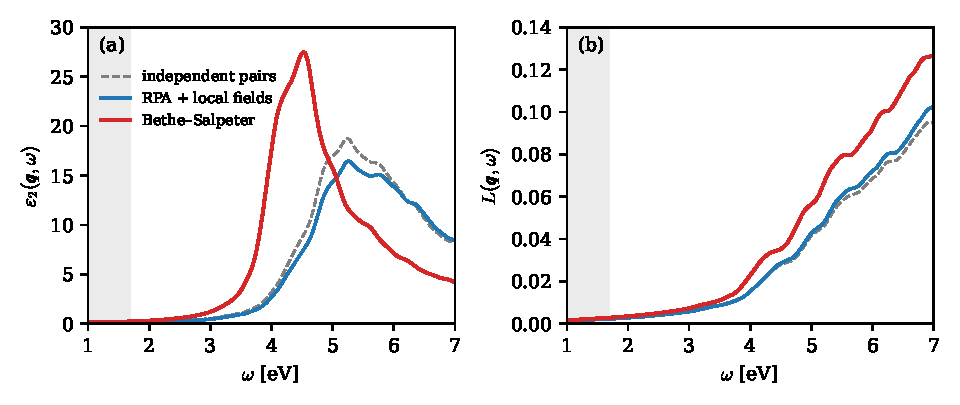
\includegraphics[width=\linewidth]{figures/ch10/fig10_4.pdf}
  \caption{The electron--hole attraction at finite momentum transfer in silicon, in a model calculation: $|\vect{q}| = \SI{0.91}{keV}$ ($0.4\times2\pi/a$) along [100]. States from the empirical pseudopotential of Cohen and Bergstresser~\cite{cohen1966band}, fitted to measured transition energies (model indirect gap \SI{0.82}{eV}; no scissor); 4 valence and 4 conduction bands on a shifted $10^3$ grid over the full zone (16{,}000 pairs); the 59 shortest reciprocal vectors in both kernels; direct kernel with the model dielectric function of Cappellini and coworkers~\cite{cappellini1993model} with $\varepsilon_\infty = 11.7$; Tamm--Dancoff resonant block with both time orderings, \cref{eq:4.9-epsmac}; Lorentzian broadening \SI{0.15}{eV}. On this grid the independent-pair spectrum agrees with a $15^3$ grid within 8 percent below \SI{6}{eV}. Gray: below the lowest pair of the grid, \SI{1.69}{eV}, where the curves are broadening tails; the bound lines are not resolved. Dashed: independent pairs (with the head screening only, in panel b); blue: random-phase approximation with local fields; red: Bethe--Salpeter equation. (a) Proper absorption $\varepsilon_2(\vect{q},\omega)$. (b) Loss function. The fitted bands already contain part of the excitonic shift, which the attraction then counts again (\cref{sec:4.9}).}
  \label{fig:10-xq}
\end{figure}

\subsection{Elliott onset and bound exciton lines}\label{sec:10.5-lines}

Near the bottom of the pair continuum at a given $\vect{q}$ the exciton form factor has a closed form, and with it the onset of \cref{eq:10.5-rate}. At fixed $\vect{q}$ the pair energy $\varepsilon_{c,\vect{k}+\vect{q}} - \varepsilon_{v\vect{k}}$ has its minimum $E_{\mathrm{min}}(\vect{q})$ of \cref{eq:3.3-Emin} at some $\vect{k}_0(\vect{q})$, and near it the pair energy rises quadratically in $\vect{k} - \vect{k}_0$, with a reduced mass set by the curvatures of the two bands at $\vect{k}_0$ and $\vect{k}_0 + \vect{q}$. This is the situation of \cref{eq:4.9-dispersion}, with the extremum of the pair energy in place of the band extrema. The relative motion obeys the hydrogenic equation \cref{eq:4.9-envelope}, and the bound states sit at $E_{\mathrm{min}}(\vect{q}) - E_x^b/n^2$. In silicon at $\vect{q} = \vect{k}_{\mathrm{c}}$ the pair minimum joins the two band extrema and $E_x^b$ is the measured \SI{14.7}{meV}. Away from the valley, $\vect{k}_0$ moves off the band extrema, the reduced mass changes, and $E_x^b$ with it (\cref{eq:E.15-disp}); we keep the symbols $E_x^b$, $a_x$ and $\mu_x$ for the values at the $\vect{q}$ in question.

When $\rho_{cv}(\vect{k},\vect{q})$ is smooth and nonzero at $\vect{k}_0$, the Elliott form \cref{eq:4.9-elliott} applies: $|\rho_{\lambda0}|^2 = \Vol|F_\lambda(0)|^2|\rho_{cv}(\vect{k}_0,\vect{q})|^2$. For the bound $s$ states, $|F_{ns}(0)|^2 = 1/(\pi a_x^3n^3)$. For the unbound states of relative momentum $\kappa$, normalized in the volume $\Vol$, $\Vol|F_{\kappa}(0)|^2$ is its free value, one, times the factor by which the attraction raises the probability of finding the electron at the hole. That factor is the Fermi factor \cref{eq:2.2-fermi} of an electron leaving a charge, with the coupling $\alpha/\varepsilon_\infty$ and the mass $\mu_x$ in place of $\alpha$ and $m_e$, so that $\xi_{\mathrm{C}} = 1/(\kappa a_x)$. With $\kappa^2 = 2\mu_x(\omega - E_{\mathrm{min}})$ and $2\mu_xE_x^ba_x^2 = 1$ from \cref{eq:4.9-WM}, the line sum in \cref{eq:10.5-rate} becomes
\begin{equation}
  \begin{aligned}
  \frac1\Vol\sum_\lambda|\rho_{\lambda0}|^2\delta(\omega - E_\lambda) = |\rho_{cv}(\vect{k}_0,\vect{q})|^2\biggl[&\sum_{n\ge1}\frac{\delta\bigl(\omega - E_{\mathrm{min}} + E_x^b/n^2\bigr)}{\pi a_x^3n^3} \\
  &+ \Theta(\omega - E_{\mathrm{min}})\,\frac{(2\mu_x)^{3/2}(\omega - E_{\mathrm{min}})^{1/2}}{4\pi^2}\,\frac{2\pi\xi_{\mathrm{C}}}{1 - \ee^{-2\pi\xi_{\mathrm{C}}}}\biggr] ,
  \end{aligned}
  \label{eq:10.5-lines}
\end{equation}
with $\xi_{\mathrm{C}} = [E_x^b/(\omega - E_{\mathrm{min}})]^{1/2}$. The density of free pairs, $\int\dd^3\kappa\,(2\pi)^{-3}\delta(\omega - E_{\mathrm{min}} - \kappa^2/2\mu_x)$, supplies the square root. The two parts meet smoothly. The lines crowd toward $E_{\mathrm{min}}$ with spacing $2E_x^b/n^3$, so their weight per unit energy tends to $1/(2\pi a_x^3E_x^b)$, and as $\omega \to E_{\mathrm{min}}^+$ the continuum tends to $(2\mu_x)^{3/2}(E_x^b)^{1/2}/2\pi$, which is the same number. The edge of the excitonic spectrum at fixed $\vect{q}$ is therefore a series of lines followed by a finite step, where independent pairs start from zero as $(\omega - E_{\mathrm{min}})^{1/2}$.

How much weight the lines take is a short calculation. Their total is $\sum_n 1/(\pi a_x^3n^3) = \zeta(3)/(\pi a_x^3)$. The free continuum without the Fermi factor holds $(2\mu_x)^{3/2}\epsilon^{3/2}/6\pi^2$ between $E_{\mathrm{min}}$ and $E_{\mathrm{min}} + \epsilon$. With $(2\mu_x)^{3/2} = 1/(a_x^3(E_x^b)^{3/2})$ the two are equal at $\epsilon = (6\pi\zeta(3))^{2/3}E_x^b = 8.0\,E_x^b$: the bound lines together carry as much weight as the free pairs within eight binding energies of the edge would have carried. The attraction does not stop there. Above the edge the Fermi factor is $6.3$ at $\omega - E_{\mathrm{min}} = E_x^b$, falls to 2.3 at $10\,E_x^b$, and is still $1 + \pi\xi_{\mathrm{C}} + \dots$ far above, a slow approach to one. The hydrogenic form of that tail is not to be trusted beyond a few tenths of an eV, where the bands stop being parabolic and the pair samples the screening at shorter distances, and the sign is all it fixes there. The spectrum it describes comes from the region near the pair minimum only. In silicon at $\vect{q} = \vect{k}_{\mathrm{c}}$ the heavy and light holes at the valence maximum each add their own copy of \cref{eq:10.5-lines}, with their own masses and vertices.

\begin{workedexample}{The exciton line of silicon below the pair onset}\label{we:10-xline}
Take a momentum transfer close to $\vect{k}_{\mathrm{c}}$ in silicon, where $E_{\mathrm{min}}$ is the gap. With the low-temperature gap of \SI{1.17}{eV} and $E_x^b = \SI{14.7}{meV}$, the $1s$ line sits at \SI{1.155}{eV} and the $2s$ line at $\SI{1.17}{eV} - E_x^b/4 = \SI{1.166}{eV}$; the radius is $a_x = \SI{4.2}{nm}$ (\cref{sec:4.9}). For a vertex that is smooth at the band extrema, \cref{eq:10.5-lines} gives the $1s$ line the weight $|\rho_{cv}|^2/(\pi a_x^3) = |\rho_{cv}|^2\times\SI{4.3e-6}{\angstrom^{-3}}$ per unit volume. It is $1/\zeta(3) = 0.83$ of all the lines, and it equals the free-pair weight within $(6\pi)^{2/3}E_x^b = 7.1\,E_x^b = \SI{0.10}{eV}$ of the edge. A particle that deposits $\omega$ between \SI{1.155}{eV} and \SI{1.17}{eV} at this $\vect{q}$ has no free pair to make and makes the exciton; one that deposits \SI{1.27}{eV} finds the free-pair density raised by the factor $2.6$. For the rate integrated over $\omega$, a line \SI{14.7}{meV} below the edge changes little; for the threshold mass it changes even less. The kinematic floor of \cref{eq:1.3-mmin}, $2\Eg/v_{\mathrm{max}}^2 = \SI{0.333}{MeV}$, becomes $2(\Eg - E_x^b)/v_{\mathrm{max}}^2 = \SI{0.329}{MeV}$, a shift of 1.3 percent, and \cref{sec:3.3} showed that this floor is not reached at all, since the momentum at which a particle that light deposits most energy falls short of the valley. Where the zero-phonon edge of silicon lies, and that its first line is weak, are the subjects of \cref{sec:13.1,sec:13.9}. The line is weak because on the valley axis the vertex at the extrema vanishes, and the $1s$ line is dark.
\end{workedexample}

\subsection{Selection rules at the zone boundary}\label{sec:10.5-rules}

Spin decides first which excitons a dark-matter coupling can make in silicon. The ground state is a singlet, the density does not act on spin, and $n_e(\vect{q})$ creates only singlet excitons, the ones of \cref{eq:4.9-bse} with $g_{\mathrm{deg}}K^{\mathrm{x}}$. The triplets, in which the electron and hole spins combine to one, are reached by the spin density and the spin current of \cref{tab:10-minimal}, and \cref{sec:10.5-triplet} treats them. Crystal momentum decides next. The lowest exciton of silicon has the electron in a valley and the hole at $\mathrm{\Gamma}$, so it carries $\vect{k}_{\mathrm{c}}$ up to a reciprocal-lattice vector, and a coupling reaches it at first order only through $\vect{q} = \vect{k}_{\mathrm{c}} + \vect{G}$. Light, with $q \approx 0$, needs a phonon (\cref{sec:6.5}). Dark matter of a few hundred keV and more carries $|\vect{k}_{\mathrm{c}}| = \SI{1.94}{keV}$ and needs none.

The symmetry of the states at the extrema decides last, and it is what makes the first line of silicon weak. Take $\vect{q} = \vect{k}_{\mathrm{c}}$ along [100], the $x$ axis, with no Umklapp vector. Consider the operations of the cubic group that leave this axis fixed: the rotations by multiples of $90^\circ$ about it and the mirrors that contain it. The conduction state at the valley minimum is invariant under all of them, and so is the operator $\ee^{\ii\vect{q}\cdot\vect{r}}$. The three valence states at the maximum transform like the products $yz$, $zx$ and $xy$ (in the notation of the band structure, $\mathrm{\Gamma}_{25'}$). Under the quarter turn about $x$, which takes $y \to z$ and $z \to -y$, $yz$ changes sign. The pair $(zx, xy)$ transforms like the two components $(z, y)$ of a vector across the axis and contains no invariant combination. A matrix element $\langle c,\vect{k}_{\mathrm{c}}|\ee^{\ii\vect{q}\cdot\vect{r}}|v,\mathrm{\Gamma}\rangle$ between an invariant state, through an invariant operator, to a state with no invariant part vanishes. Half of these operations carry the fractional translation of the diamond structure (\cref{app:C.17}), which multiplies the Bloch states and the operator by phases; for $\vect{q} = \vect{k}_{\mathrm{c}}$ exactly, the phase of the operator, $\ee^{-\ii\vect{q}\cdot\vect{\tau}_2}$, cancels that of the conduction state, $\ee^{-\ii\vect{k}_{\mathrm{c}}\cdot\vect{\tau}_2}$, and the argument stands. In germanium the valleys lie along [111]. The rotations by $120^\circ$ about that axis and the mirrors containing it leave the combination $yz + zx + xy$ invariant, and the vertex at the extrema does not vanish.

A vertex that vanishes at the extrema grows linearly away from them: $\rho_{cv}(\vect{k},\vect{q}) \simeq (\vect{k} - \vect{k}_0)\cdot\vect{g}$ with $\vect{g} = \nabla_{\vect{k}}\rho_{cv}$, and $\vect{q}$ itself off the axis adds a term proportional to its distance $\delta q_\perp$ from it. Transitions with a vertex of this kind are called second class~\cite{elliott1957intensity}. Their exciton form factor picks out the gradient of the envelope where the electron meets the hole. From $A_{\vect{k}} = \Vol^{-1/2}\int\dd^3r\,F(\vect{r})\ee^{-\ii\vect{k}\cdot\vect{r}}$, $\sum_{\vect{k}}A_{\vect{k}}\,\vect{k}\cdot\vect{g} = -\ii \Vol^{1/2}\,\vect{g}\cdot\nabla F(0)$, which vanishes for $s$ states and is nonzero for the $p$ state oriented along $\vect{g}$. Its envelope is $R_{n1}(r)\,(3/4\pi)^{1/2}\cos\theta$, with $\theta$ measured from $\vect{g}$, and the hydrogen radial function starts as $R_{n1} \to \tfrac23[(n^2 - 1)/n^5]^{1/2}r/a_x^{5/2}$; for $n = 2$ this is $R_{21} = r\,\ee^{-r/2a_x}/(2\sqrt6\,a_x^{5/2})$. So $|\vect{g}\cdot\nabla F_{np}(0)|^2 = |\vect{g}|^2(n^2 - 1)/(3\pi a_x^5n^5)$, and in place of the $s$ lines of \cref{eq:10.5-lines},
\begin{equation}
  \frac1\Vol\sum_{\lambda\in\text{lines}}|\rho_{\lambda0}|^2\delta(\omega - E_\lambda) = |\nabla_{\vect{k}}\rho_{cv}|^2\sum_{n\ge2}\frac{n^2 - 1}{3\pi a_x^5n^5}\,\delta\bigl(\omega - E_{\mathrm{min}} + E_x^b/n^2\bigr) \qquad\text{(second class)} .
  \label{eq:10.5-second}
\end{equation}
There is no $1s$ line. The first line is $2p$, at $E_x^b/4 = \SI{3.7}{meV}$ below the continuum. Against an allowed $1s$ line with a vertex of size $|\rho|$ it is weaker by $(|\nabla_{\vect{k}}\rho_{cv}|/|\rho|)^2/(32a_x^2)$, a factor of about $10^{-3}$ for a vertex that changes by order one across a tenth of the zone ($|\nabla_{\vect{k}}\rho_{cv}|/|\rho| \approx \SI{9}{\angstrom}$). The continuum changes the same way. Its vertex is $|\vect{g}\cdot\vect{\kappa}|^2$, or $|\vect{g}|^2\kappa^2/3$ averaged over directions, so the free pairs start as $(\omega - E_{\mathrm{min}})^{3/2}$. The $p$-wave Coulomb function at the origin carries the extra factor $1 + \xi_{\mathrm{C}}^2$, from $|\Gamma(2 + \ii\xi_{\mathrm{C}})|^2 = (1 + \xi_{\mathrm{C}}^2)|\varGamma(1 + \ii\xi_{\mathrm{C}})|^2$, which keeps the step at the edge finite. Off the axis the $1s$ line returns with a weight proportional to $\delta q_\perp^2$, and in a rate averaged over directions it enters at the energy of the $1s$ line with a weight that grows from zero.

The rule holds only for $\vect{q} = \vect{k}_{\mathrm{c}}$ without an Umklapp vector. With $\vect{q} = \vect{k}_{\mathrm{c}} + \vect{G}$ the phases of the shifted operations no longer cancel, $\ee^{-\ii\vect{G}\cdot\vect{\tau}_2}$ can be $-1$, and transitions that are forbidden at $\vect{G} = 0$ become allowed. Which classes open, at what momenta and with what strength, follows from the glide symmetry of \cref{app:C.17} and is worked out in \cref{sec:13.9}, where it decides the zero-phonon edge of silicon. Spin--orbit coupling lifts the zero on the axis as well, by an amount too small to matter (\cref{sec:13.9}).

\subsection{Time orderings and the coupling block}\label{sec:10.5-orderings}

A dark-matter calculation with excitons must give the loss function, not only the absorption $\varepsilon_2$, and the loss function needs the real part of the dielectric function as well. Here the way the equation is solved matters more than one might expect. \Cref{eq:4.9-epsmac} has two terms for each exciton, a resonant pole at $+E_\lambda$ and an antiresonant one at $-E_\lambda$. The second is the same process with the opposite time ordering, the pair annihilated before it is created, and it is the mirror image that causality requires: with both terms, $\varepsilon_{\mathrm{mac}}(\vect{q},\omega)$ is analytic in the upper half plane and obeys the Kramers--Kronig relations of \cref{app:C.5}. A program that solves the resonant block alone, as the Tamm--Dancoff approximation does, can still form the response with both orderings; this is the retarded Tamm--Dancoff form, and \cref{eq:4.9-epsmac} is written that way. If instead the antiresonant term is dropped altogether, the response is resonant-only.

At $\omega > 0$ the antiresonant term has no imaginary part, so the two forms have the same $\varepsilon_2$. Their real parts, however, differ. With $\varepsilon_2 = \pi C\sum_\lambda w_\lambda\delta(\omega - E_\lambda)$ for the weights $w_\lambda$ and the positive constant $C$ of \cref{eq:4.9-epsmac}, the two orderings give $\varepsilon_1 - 1 = C\sum_\lambda w_\lambda[1/(E_\lambda - \omega) + 1/(E_\lambda + \omega)]$, and the resonant term alone gives $\varepsilon_1^{\mathrm{res}} - 1 = C\sum_\lambda w_\lambda/(E_\lambda - \omega)$. Written with $\varepsilon_2$,
\begin{equation}
  \varepsilon_1 - 1 = \frac2\pi\,\mathrm{P}\!\int_0^\infty\dd\omega'\,\frac{\omega'\varepsilon_2(\omega')}{\omega'^2 - \omega^2} , \qquad
  \varepsilon_1^{\mathrm{res}} - 1 = \frac1\pi\,\mathrm{P}\!\int_0^\infty\dd\omega'\,\frac{\varepsilon_2(\omega')}{\omega' - \omega} ,
  \label{eq:10.5-kk}
\end{equation}
the first being \cref{eq:C.5-KKeps}. For a single oscillator at $E_0$ the ratio is
\begin{equation}
  \frac{\varepsilon_1^{\mathrm{res}} - 1}{\varepsilon_1 - 1} = \frac{E_0 + \omega}{2E_0} , \qquad
  \frac{L^{\mathrm{res}}}{L} = \frac{\varepsilon_1^2 + \varepsilon_2^2}{(\varepsilon_1^{\mathrm{res}})^2 + \varepsilon_2^2} \simeq \Bigl(\frac{\varepsilon_1}{\varepsilon_1^{\mathrm{res}}}\Bigr)^2 \quad (\varepsilon_2 \ll \varepsilon_1) .
  \label{eq:10.5-res}
\end{equation}
At $\omega \to 0$ the resonant-only form keeps half of $\varepsilon_1 - 1$. In silicon at small $q$, with $\varepsilon_1 = 11.7$, it overstates the loss function by $[2\varepsilon_1/(\varepsilon_1 + 1)]^2 = 3.4$ as $\omega \to 0$ (at \SI{1.3}{eV} and the smallest momentum of the tables below, \SI{0.49}{keV}, the factor is 2.2), and wherever $\varepsilon_1$ is large and $\varepsilon_2$ small, as below and just above the gap, the error is typically a factor of two. It vanishes as $q \to \infty$, where $\varepsilon_1 \to 1$ and screening disappears.

The silicon tables of \cref{sec:10.2} put numbers on this. From their $\varepsilon_2$ with local fields, \cref{eq:10.5-kk} reproduces the tabulated static $\varepsilon(\vect{q},0)$ to within one percent at every $q$, which shows that the tables hold enough of the spectrum for the transform. At $|\vect{q}| = \SI{1.39}{keV}$ ($\SI{0.71}{\angstrom^{-1}}$) and $\omega = \SI{1.3}{eV}$, below the pair continuum at that momentum, $\varepsilon_1 = 4.45$ and $\varepsilon_1^{\mathrm{res}} = 3.05$, and the resonant-only form overstates $L$ by a factor of 2.12. A single oscillator that carries the whole valence $f$-sum and reproduces the static value 4.31, $E_0 = \omega_p^{\mathrm{val}}/[\varepsilon(\vect{q},0) - 1]^{1/2} = \SI{9.1}{eV}$ with $\omega_p^{\mathrm{val}} = \SI{16.6}{eV}$, gives 2.23 from \cref{eq:10.5-res}, and the model dielectric function of \cref{sec:10.2} gives 2.25. These momenta and energies are those at which the phonon-assisted pairs of \cref{sec:13.3} are made, and that is where the factor of two would land. It falls to 1.53 at $q_0 = \SI{3.73}{keV}$ and to 1.07 at \SI{8}{keV}, and it is within 15 percent of one above \SI{6.7}{keV}. A resonant-only evaluation is harmless for heavy mediators at masses where large $q$ dominates, and wrong by a factor of two for light mediators and light dark matter.

The retarded form has no such error, but it still drops something: the coupling block of \cref{eq:D.12-blocks}, which mixes the creation of one pair with the annihilation of another. Its effect follows from a single pair of transition energy $\Delta$ coupled to itself by a kernel $K$ in both blocks. With coupling the poles are at $\pm E_{\mathrm{cp}}$, $E_{\mathrm{cp}}^2 = (\Delta + K)^2 - K^2 = \Delta(\Delta + 2K)$, so $E_{\mathrm{cp}} = \Delta + K - K^2/2\Delta + \dots$; without it they are at $\pm(\Delta + K)$. The energy is wrong only at second order, the statement of \cref{sec:4.9}. The weight is not. With $R^0(0) = -2|\rho|^2/\Delta$ for the free pair, the static response of the coupled pair is $R(0) = R^0/(1 - KR^0/|\rho|^2) = -2|\rho|^2/(\Delta + 2K)$. The retarded resonant block gives $R^{\mathrm{TD}}(0) = -2|\rho|^2/(\Delta + K)$, and
\begin{equation}
  \frac{R^{\mathrm{TD}}(0)}{R(0)} = \frac{\Delta + 2K}{\Delta + K} = 1 + \frac{K}{\Delta + K} ,
  \label{eq:10.5-coupling}
\end{equation}
an error of first order in the kernel, here written for an exchange-type $K$ that enters the coupling block with the same sign as the resonant one. Which kernel remains in the coupling block depends on how the long-range part is handled. The head of the exchange kernel, the term at $\vect{G}_q$, is the macroscopic field, and it turns the proper response into the screened one (\cref{sec:4.9}). If it is kept in the Bethe--Salpeter Hamiltonian and the coupling block is dropped, the screening itself is computed in the Tamm--Dancoff approximation, and for the screened $L$ the error is set by $v_{\mathrm{C}}(q)$, large at small $q$. The safe arrangement is the one of \cref{app:E.15}: the Tamm--Dancoff equation, without the head, for the proper $\varepsilon_2$ with its lines, and the screening from the full response, with both orderings, through $L = \varepsilon_2/|\varepsilon_{\mathrm{mac}}|^2$ and \cref{eq:10.5-kk}. The coupling block then still holds the local-field exchange and the small interband part of the direct kernel. Since the local fields change $\varepsilon_2$ of silicon by about ten percent (\cref{sec:4.6}), the remaining error is of that size, about \SI{10}{\percent} on the proper $\varepsilon_2$. In the model of \cref{fig:10-xq}, where the coupling block holds the local-field exchange alone, the full random-phase response with local fields differs from its retarded Tamm--Dancoff form by 2.6 percent of the peak of $\varepsilon_2$. The \SI{10}{\percent} is an estimate; the full coupled calculation, which also restores the $f$-sum rule that the Tamm--Dancoff form strains, is part of \cref{app:E.15}.

The static screened interaction is the other approximation in the equation. It holds when the binding energies and the spread of transition energies that matter are small against the frequencies at which $\varepsilon^{-1}$ changes, the plasma frequency of \SI{16.6}{eV} in silicon (\cref{sec:4.9}). For bound lines of \SI{14.7}{meV} and pairs within a few eV of the gap this holds, and the dynamical screening of the interaction, left for the full calculation of \cref{app:E.15}, is not expected to rival the two errors above.

\begin{limitbox}[Bethe--Salpeter exciton rate][lim:10.5a]
With the loss function of the Bethe--Salpeter equation in the Tamm--Dancoff approximation, the rate is \cref{eq:10.2-rate} with $\bar L = \Imag[-1/\varepsilon_{\mathrm{mac}}^{\mathrm{BSE}}(q,\omega)]$, or \cref{eq:10.5-rate} line by line~\cite[Eqs.~(1) and (2)]{taufertshofer2026excitonic}.
\par\smallskip
{\centering
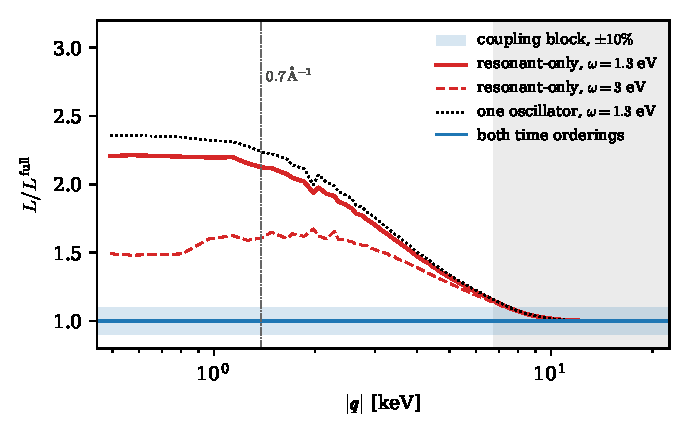
\includegraphics[width=0.82\linewidth]{figures/ch10/limit10_5a.pdf}
\captionof{figure}{Loss function of silicon in two evaluations of the same response, divided by the evaluation with both time orderings, against $|\vect{q}|$. Red: resonant-only real part, \cref{eq:10.5-kk}, at $\omega = \SI{1.3}{eV}$ (solid) and \SI{3}{eV} (dashed), from $\varepsilon_2$ of the random-phase tables with local fields of \cref{sec:10.2} (threshold \SI{1.11}{eV}, the step-model gap that accompanies them; directions averaged in bins of \SI{100}{eV}). Dotted: a single oscillator with the valence $f$-sum and the tabulated static $\varepsilon(q,0)$, \cref{eq:10.5-res}, at \SI{1.3}{eV}. Blue line and band: both time orderings, with the estimated $\pm\SI{10}{\percent}$ error of the coupling block, \cref{eq:10.5-coupling}. Dash-dotted: $|\vect{q}| = \SI{0.7}{\angstrom^{-1}}$ (\SI{1.39}{keV}), the momentum of the numbers quoted in the text. Gray: momenta at which the resonant-only form is within \SI{15}{\percent}, $|\vect{q}| \ge \SI{6.7}{keV}$.}\label{fig:10-bse-limit}
\par}
\smallskip
Below about \SI{7}{keV}, where screening is strong, a resonant-only real part overstates the loss function by up to a factor of two or more; with both time orderings the remaining error is that of the coupling block.
\end{limitbox}

\subsection{Triplet excitons}\label{sec:10.5-triplet}

A coupling to the electron spin, such as $\mathcal{O}_4$ of \cref{tab:8-operators}, creates the electron--hole pair with its spins combined to one, a triplet, and the triplet rows of \cref{tab:10-minimal} are its responses. Without interaction they are a quarter of the density response (\cref{eq:D.30-quarter}), and they are not screened (\cref{sec:10.4}). With the interaction the triplet pair has its own Bethe--Salpeter equation. The exchange kernel comes from a pair that annihilates and is re-created, and a spin-one pair cannot annihilate into the spinless density that the Coulomb line couples to, so its contribution cancels between the two spin projections. The direct kernel, the attraction between the electron and the hole, acts in every spin state alike. The triplet Hamiltonian is therefore
\begin{equation}
  H^{\mathrm{exc}}_{\mathrm{T}} = \Delta - K^{\mathrm{d}} ,
  \label{eq:10.5-triplet}
\end{equation}
\cref{eq:4.9-bse} with $g_{\mathrm{deg}}K^{\mathrm{x}}$ removed, and the spin structure factor follows from its eigenpairs as the density one does, with the vertex $\sigma^z/2$ in place of one and no $1/|\varepsilon_{\mathrm{mac}}|^2$.

The bound lines of the triplet sit where the singlet ones do, up to the electron--hole exchange splitting. That splitting is the short-range exchange of a pair whose electron and hole meet in one cell with probability of order $(a/a_x)^3$, $2\times10^{-3}$ in silicon, so it is a fraction of order $10^{-3}$ of the binding, well below a meV. And the Wannier analysis above, which used only $K^{\mathrm{d}}$, applies unchanged: the triplet edge has the same lines, the same Fermi factor and the same selection rules of point symmetry as the singlet one, with the spin vertex in place of the density vertex. What separates the two channels is the rest of $K^{\mathrm{x}}$, the local fields, which raise the singlet transitions and move weight up (\cref{sec:4.6}) and which the triplet lacks. In the model of \cref{fig:10-xq}, the triplet spectrum below \SI{3}{eV} carries 2.2 times the independent-pair weight, and between 2.5 and \SI{4}{eV} five times, while above \SI{4}{eV} the two agree within 4 percent. The attraction alone moves the triplet weight down more than the singlet's, since no local fields push back.

What is not known is the triplet response at keV momentum transfers beyond independent particles: the ladder with the screened attraction over the whole spectrum, together with the exchange--correlation kernel of the spin channel, which is not the one of the density. As an estimate, near the edge the spin rows of \cref{tab:10-minimal} inherit the excitonic enhancement of the singlet ones, without their local fields and without screening. \Cref{app:E.16} specifies the calculation, as the Bethe--Salpeter run of \cref{app:E.15} with the exchange kernel switched off; its control is the limit without interaction, which must return a quarter of the independent-particle density response.

\subsection{Open problems}\label{sec:10.5-open}

For silicon and germanium no finite-momentum Bethe--Salpeter calculation exists, with or without the coupling block, and no calculation resolves the bound lines of an indirect gap. The lines need grids around the pair minimum far finer than a uniform grid can afford, and are therefore to be added from \cref{eq:10.5-lines,eq:10.5-second} with computed masses, vertices and vertex gradients. The full coupled calculation would settle the \SI{10}{\percent} of \cref{eq:10.5-coupling}, test the factor of two of \cref{eq:10.5-res} directly, and check the $f$-sum rule to a percent (\cref{app:E.15}). The triplet response beyond independent particles is open as stated above.

So is the response of crystals in which the exciton is not large. In NaI the lowest excitons are compact, of the size of an ion pair, and the hole localizes on two anions while the lattice relaxes around it: the exciton becomes self-trapped. The Wannier picture fails, and the line that dark matter creates is dressed by the phonons that the relaxation emits. Take linear coupling, a harmonic lattice and a vertex independent of the lattice coordinates. The line at $E_\lambda$ then becomes a Poisson series of replicas spaced by a mean phonon energy $\bar\omega$, with the weight $\ee^{-S_{\mathrm{HR}}}S_{\mathrm{HR}}^n/n!$ in the $n$th (\cref{eq:E.15-ste}), where the Huang--Rhys factor $S_{\mathrm{HR}}$ is the mean number of phonons emitted, the relaxation energy divided by $\bar\omega$. For NaI none of $S_{\mathrm{HR}}$, $\bar\omega$ or the form factor $\rho_{\lambda0}(\vect{q})$ is known at keV momenta, and \cref{app:E.15} specifies their calculation. The localized (Frenkel) exciton itself, the limit of a pair confined to one site, is made precise in \cref{sec:16.4}. The spread between the random-phase and the excitonic rate near the gap, the factor that a resonant-only evaluation can introduce, and the coupling error enter the many-body uncertainty of \cref{sec:8.8}, collected for this chapter in \cref{sec:10.10}.

\section{Core and relativistic states}\label{sec:10.6}

A germanium atom has 32 electrons, and the band structure of \cref{sec:10.1} follows four of them. Ten more sit in the $3d$ shell, \SI{29.4}{eV} below the valence-band maximum, close enough for light dark matter to excite them, and the deeper shells follow at \SI{122}{eV} and beyond. \Cref{sec:3.5} found where each shell becomes kinematically accessible and why the momenta it needs are large: an electron that absorbs $\omega$ must receive at least $q = \omega/v_{\mathrm{max}}$, \SI{11}{keV} for germanium $3d$ and \SI{38}{keV} for silicon $2p$. It left two questions for the rate. At which momentum transfer does a core shell actually take over from the valence electrons, given that both are probed far out in the tails of their momentum distributions? And how much do the relativistic corrections of order $(Z\alpha)^2$, which grow with the depth of the shell, change the response there? We answer both for silicon and germanium, and find the three hypotheses under which the response of the core electrons separates from that of the valence electrons: a filled shell, a flat band and orthogonal site orbitals.

\subsection{Core shells within kinematic reach}\label{sec:10.6-reach}

The structure factor of a crystal with core shells is the sum of the valence term of \cref{eq:10.1-S0} and one term per core shell. The core states of atom $\kappa$ in the cell are the Bloch sums $\psi_{\kappa nlm,\vect{k}}$ of \cref{eq:E.7-core}, with the energy $-E_{\mathrm{core}}$ measured from the valence maximum, and their vertex with a conduction state is $\rho_{c,\kappa nlm}(\vect{k},\vect{q}) = \langle\psi_{c,\vect{k}+\vect{q}}|\ee^{\ii\vect{q}\cdot\vect{r}}|\psi_{\kappa nlm,\vect{k}}\rangle$. Following the steps of \cref{eq:10.1-S0} with these states in place of the valence bands,
\begin{equation}
  S^0_{\mathrm{core}}(\vect{q},\omega) = 4\pi\sum_{\kappa nlm}\sum_c\int_{\mathrm{BZ}}\frac{\dd^3k}{(2\pi)^3}\,|\rho_{c,\kappa nlm}(\vect{k},\vect{q})|^2\,\delta\bigl(\omega - \varepsilon_{c,\vect{k}+\vect{q}} - E_{\mathrm{core},\kappa nl}\bigr) .
  \label{eq:10.6-core}
\end{equation}
Both states in the vertex must be all-electron states. The core orbital is all-electron by construction. The conduction state must carry its core-region oscillations, which the reconstruction \cref{eq:3.5-rhoAE} restores, because the overlap with a core orbital is taken inside the sphere where a pseudo-wavefunction is wrong. A semicore shell kept in the valence of the pseudopotential, such as germanium $3d$, enters \cref{eq:10.1-S0} instead, with reconstructed vertices on both sides. Griffin and coworkers computed the germanium $3d$ contribution both ways and found that the atomic orbitals reproduce the reconstructed crystal states up to the largest momentum the crystal calculation resolves, about \SI{45}{keV}~\cite[Sects.~2.2 and~3.3]{griffin2021extended}.

How many core electrons can dark matter reach at a given $q$? A momentum transfer $q$ deposits at most $qv_{\mathrm{max}}$, whatever the mass (\cref{eq:1.3-vmin}), so the relevant measure is the part of the structure factor below that energy. Per atom and per shell we define
\begin{equation}
  N^{\mathrm{acc}}_{nl}(q) = \int_{\Eg + E_{\mathrm{core}}}^{qv_{\mathrm{max}}}\dd\omega\;S^{\mathrm{at}}_{nl}(q,\omega) ,
  \label{eq:10.6-Nacc}
\end{equation}
where $S^{\mathrm{at}}_{nl}(q,\omega)$ is the response of one atom's shell, normalized so that its integral over all $\omega$ is the occupation $N_{nl}$ when $q$ is large (closure, \cref{sec:4.3}). The structure factor of \cref{eq:10.6-core} is $(2\pi/\Omega)\sum_\kappa S^{\mathrm{at}}_{\kappa nl}$, as the next subsection shows, so $N^{\mathrm{acc}}_{nl}$ counts the electrons of a shell, per atom, that the halo can excite at momentum transfer $q$. With plane-wave final states the shell response follows from the ionization form factor of \cref{sec:2.2}. The number of final states per unit ejected energy is $|f_{\mathrm{ion}}|^2/4E_{\mathrm{ej}}$, and \cref{eq:2.2-fion-pw}, with the radial momentum orbital $\phi_{nl}(k)$ of \cref{sec:3.5} normalized to $\int k^2\phi_{nl}^2\,\dd k = 1$, gives
\begin{equation}
  S^{\mathrm{at}}_{nl}(q,\omega) = \frac{N_{nl}}{2}\,\frac{m_e}{q}\int_{|p - q|}^{p + q}k\,\phi_{nl}(k)^2\,\dd k , \qquad p = [2m_e(\omega - E_{\mathrm{core}})]^{1/2} ,
  \label{eq:10.6-Sat}
\end{equation}
for a full shell, $N_{nl} = 2(2l + 1)$, and for the spherical average of a partly filled valence shell. The final kinetic energy is counted from the valence maximum, as for the free final states of Griffin and coworkers~\cite[Eq.~(3.21)]{griffin2021extended}. Integrating over $\omega$, with $\dd\omega = p\,\dd p/m_e$ and the order of integration exchanged, each $k$ collects $\int_{|k - q|}^{k + q}p\,\dd p = 2kq$, and the integral is $N_{nl}\int k^2\phi_{nl}^2\,\dd k = N_{nl}$: closure holds.

\Cref{eq:10.6-Sat} explains when a shell takes over. Near its opening the ejected momentum $p$ is much smaller than $q$, the integral is $2pq\,\phi_{nl}(q)^2$, and
\begin{equation*}
  N^{\mathrm{acc}}_{nl}(q) \simeq N_{nl}\,m_e\,\phi_{nl}(q)^2\int_{E_{\mathrm{core}}}^{qv_{\mathrm{max}}}p\,\dd\omega = \frac{2\sqrt2}{3}\,N_{nl}\,m_e^{3/2}\,\phi_{nl}(q)^2\,(qv_{\mathrm{max}} - E_{\mathrm{core}})^{3/2} ,
\end{equation*}
where the gap has been dropped from the lower limit. Two factors decide. The first is the number of electrons of the shell per unit volume of momentum at $p = q$, $N_{nl}\phi_{nl}(q)^2$, in which a core shell beats the valence above about \SI{5}{keV} (\cref{fig:3-core}). The second is the phase space $(qv_{\mathrm{max}} - E_{\mathrm{core}})^{3/2}$, which is zero at the opening and approaches that of the valence, $(qv_{\mathrm{max}})^{3/2}$, only once $qv_{\mathrm{max}}$ is several times $E_{\mathrm{core}}$. A core shell therefore overtakes the valence a little above its opening, at the momentum where its larger density outweighs the reduced phase space.

\Cref{fig:10-core} evaluates \cref{eq:10.6-Nacc} for germanium. The core and semicore shells use the free-atom orbitals of \cref{fig:3-core}. The valence uses the crystal: the independent-particle $\varepsilon_2$ of Knapen, Kozaczuk and Lin~\cite[Sect.~III\,B]{knapen2021dark}, from which $S = (2q^2/e^2)\varepsilon_2$ (\cref{sec:10.2}) and, per atom of the two-atom cell, $S^{\mathrm{at}} = q^2\Omega\varepsilon_2/8\pi^2\alpha$. That table holds only the four valence electrons, with the $3d$ shell frozen, on bands scissored to the measured gap at zero temperature. It ends at \SI{22.5}{keV}, where its plane-wave basis ends too, and we use it up to \SI{15}{keV} and \cref{eq:10.6-Sat} with the atomic $4s$ and $4p$ orbitals above. At the switch the two differ by 27 percent. Between 5 and \SI{15}{keV} the atomic model and the crystal tables of silicon and germanium differ by up to a factor of six in either direction, since the low-energy corner $\omega \le qv_{\mathrm{max}}$ is where the band structure matters most. That is the accuracy of the valence curve beyond the table.

\begin{figure}[tbp]
  \centering
  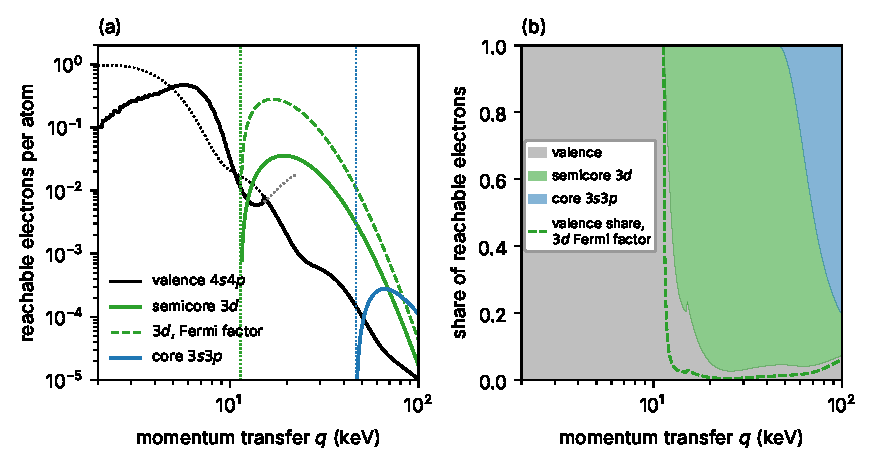
\includegraphics[width=\linewidth]{figures/ch10/fig10_5.pdf}
  \caption{Germanium electrons that dark matter of any mass can excite at momentum transfer $q$, that is, with energy deposits between the threshold of the shell and $qv_{\mathrm{max}}$, $v_{\mathrm{max}} = 2.650\times10^{-3}$. (a)~Electrons per atom, $N^{\mathrm{acc}}_{nl}(q)$ of \cref{eq:10.6-Nacc}, for the valence shell (black), the semicore $3d$ shell (green) and the core $3s$ and $3p$ shells (blue). Valence: crystal independent-particle response of Knapen, Kozaczuk and Lin (PAW, $3d$ frozen) below \SI{15}{keV}; above, the plane-wave model of \cref{eq:10.6-Sat} with the free-atom $4s$, $4p$ orbitals (dotted lines continue each curve past the switch). Core and semicore: \cref{eq:10.6-Sat} with free-atom, scalar-relativistic PBE orbitals and plane-wave final states whose kinetic energy is counted from the valence maximum; dashed, the $3d$ shell with the Fermi factor of \cref{eq:2.2-fermi} at $Z_{\mathrm{eff}} = 1$. Dotted vertical lines: the openings $(\Eg + E_{\mathrm{core}})/v_{\mathrm{max}}$ of the $3d$ and $3p$ shells, with centroid binding energies 29.4 and \SI{122.2}{eV} and $\Eg = \SI{0.744}{eV}$. Germanium $2s$, $2p$ and $1s$ open above \SI{460}{keV}. (b)~Shares of the reachable electrons: valence (gray), $3d$ (green), $3s3p$ (blue); dashed, the valence share when the $3d$ shell carries the Fermi factor. The $3d$ shell overtakes the valence at \SI{12.5}{keV} (\SI{11.5}{keV} with the Fermi factor) and holds more than 90 percent of the reachable electrons from 20 to \SI{50}{keV}.}
  \label{fig:10-core}
\end{figure}

The figure answers the first question for germanium. Below \SI{11.3}{keV} only the valence is reachable, and its count falls from 0.44 electrons per atom at \SI{5}{keV} to 0.03 at \SI{10}{keV} as the window $\omega \le qv_{\mathrm{max}}$ moves into the low-energy tail of a spectrum that is centered on $q^2/2m_e$. The $3d$ shell opens at \SI{11.3}{keV} and overtakes the valence at \SI{12.5}{keV}. By \SI{20}{keV} it holds 0.036 reachable electrons per atom against 0.002 for the valence, and it keeps more than 90 percent of the total until the $3p$ and $3s$ shells, opening at 46 and \SI{68}{keV}, take over near \SI{69}{keV}. For silicon the same model puts the opening of $2p$ at \SI{38}{keV} and its crossing with the valence at \SI{46}{keV}, and the $2s$ shell overtakes $2p$ near \SI{77}{keV}. Since the silicon valence count there comes from the atomic model, uncertain by a factor of a few, and the $2p$ count rises steeply above its opening, the crossing is uncertain by a few keV.

Two features of the model need checking, the non-orthogonality of plane-wave final states and the missing Coulomb attraction of the ion. A plane wave is not orthogonal to the bound orbital. Its projection onto the initial orbital adds a spurious term of relative size $|F_{nl}(q)|^2\phi_{nl}(p)^2/\langle\phi_{nl}(|\vect{p} - \vect{q}|)^2\rangle$, with $F_{nl}(q)$ the elastic form factor of the shell; for germanium $3d$ between 12 and \SI{30}{keV} it stays below 6 percent. The final state is the larger issue. A slow electron leaving a core region is pulled toward the ion, and the Fermi factor, 12 at a final momentum of \SI{2}{keV} and 5 at \SI{5}{keV} for $Z_{\mathrm{eff}} = 1$, raises the $3d$ count by about that much near the edge (dashed curves). This moves the crossing only from 12.5 to \SI{11.5}{keV}, because the count rises so steeply above the opening, but it changes the size of the $3d$ contribution to a rate by an order of magnitude. Crystal conduction states, as in Griffin's calculation, are the correct final states, and the Fermi factor only brackets them.

\begin{workedexample}{The germanium $3d$ onset in $q$}\label{we:10-ge3d}
The $3d$ shell is a doublet, $3d_{5/2}$ at \SI{29.2}{eV} and $3d_{3/2}$ at \SI{29.8}{eV} below the valence maximum~\cite[Table~1-1]{williams2009electron}. With $\Eg = \SI{0.744}{eV}$ the thresholds are 29.94 and \SI{30.54}{eV}, and the openings $(\Eg + E_{\mathrm{core}})/v_{\mathrm{max}}$ are \SI{11.3}{keV} and \SI{11.5}{keV}. The threshold masses $2(\Eg + E_{\mathrm{core}})/v_{\mathrm{max}}^2$ are 8.5 and \SI{8.7}{MeV}; the rounded values of \cref{sec:3.5}, \SI{11}{keV} and \SI{8.5}{MeV}, are those of a single level at \SI{29}{eV}.

Opening is not taking over. Just above \SI{11.3}{keV} the window $qv_{\mathrm{max}} - E_{\mathrm{core}}$ is a fraction of an eV wide, and the $3d$ count of \cref{eq:10.6-Nacc} starts from zero. From \cref{fig:10-core}a, at \SI{12}{keV} the $3d$ shell offers 0.0040 reachable electrons per atom against 0.0084 for the valence, at \SI{15}{keV} 0.025 against 0.0065. The two are equal at \SI{12.5}{keV} with the crystal valence. With the atomic valence the crossing is at \SI{13.1}{keV}, and with the Fermi factor on the $3d$ final states at \SI{11.5}{keV}. The onset in $q$ is therefore
\begin{equation*}
  q_{3d} \simeq (12.5 \pm 1)\,\mathrm{keV} = (3.3 \pm 0.3)\,q_0 ,
\end{equation*}
with $q_0 = \alpha m_e = \SI{3.73}{keV}$. Three quarters of the $3d$ electrons have momenta above \SI{11}{keV} (\cref{sec:3.5}), so the shell is probed near the peak of its distribution, while the valence is probed far in its tail.

Which masses use this momentum? A momentum transfer $q$ with energy deposited $\omega$ needs $\vmin = \omega/q + q/2\mchi \le v_{\mathrm{max}}$ (\cref{eq:1.3-vmin}), so at the $3d_{5/2}$ threshold, $\omega = \SI{29.94}{eV}$,
\begin{equation*}
  \mchi \ge \frac{q}{2(v_{\mathrm{max}} - \omega/q)} = \frac{\SI{12.5}{keV}}{2\,(2.650 - 2.395)\times10^{-3}} = \SI{25}{MeV} ,
\end{equation*}
and \SI{19}{MeV} for $q = \SI{13}{keV}$. A particle of \SI{10}{MeV} reaches the $3d_{5/2}$ edge only for $q$ between 16 and \SI{37}{keV}, where the $3d$ shell dominates the reachable electrons but only the fastest particles of the halo contribute, through the tail of $\eta(\vmin)$. Weighting each $(q,\omega)$ with $\eta(\vmin)$ as in the heavy-mediator rate \cref{eq:1.5-rate}, with a one-pair threshold and the valence from the crystal table below \SI{22.5}{keV} and the atomic model above, gives the ratio of the $3d$ rate to the valence rate. In the plane-wave model it is $6\times10^{-5}$ at \SI{10}{MeV}, 0.07 at \SI{30}{MeV}, 0.27 at \SI{100}{MeV} and 0.34 at \SI{1}{GeV}. With the Fermi factor it is $1\times10^{-3}$, 0.69, 2.1 and 3.4. Griffin and coworkers, with crystal conduction states, find the $3d$ term dominant for a heavy mediator above about \SI{30}{MeV} at a one-pair threshold, and at lower masses for higher thresholds~\cite[Sect.~4.1]{griffin2021extended}. The onset in $q$ is robust to the final state; the mass at which the $3d$ shell dominates the rate is not, and only a calculation with crystal final states fixes it.
\end{workedexample}

\subsection{Separation of core and valence responses}\label{sec:10.6-factor}

The core term \cref{eq:10.6-core} is a double sum over $\vect{k}$ and the orbitals $m$ of every atom, and one might expect interference between the orbitals of neighboring atoms, with phases $\ee^{\ii\vect{q}\cdot(\vect{\tau}_\kappa - \vect{\tau}_{\kappa'})}$. There is none, under three conditions. First, the shell is completely filled. Second, its band is flat on the scale of the energies that the response resolves, so that all its states share one energy $-E_{\mathrm{core}}$. Third, the atomic orbitals of different sites are orthogonal. For a final state $|f\rangle$ the sum over the initial states of the shell is then $\sum_i|\langle f|\ee^{\ii\vect{q}\cdot\vect{r}}|i\rangle|^2 = \langle f|\ee^{\ii\vect{q}\cdot\vect{r}}P_{nl}\ee^{-\ii\vect{q}\cdot\vect{r}}|f\rangle$, with $P_{nl}$ the projector on the shell. A projector does not depend on the basis that spans it, and in the basis of the atomic orbitals $\psi^{\mathrm{at}}_{\vect{R}\kappa nlm}$ of \cref{eq:E.7-core}, centered on the atom $\kappa$ of cell $\vect{R}$, it is $\sum_{\vect{R}\kappa m\sigma}|\psi^{\mathrm{at}}_{\vect{R}\kappa nlm}\sigma\rangle\langle\psi^{\mathrm{at}}_{\vect{R}\kappa nlm}\sigma|$. The sum over initial states is a sum of squares, one per site, with no cross terms. Every cell gives the same contribution by translation symmetry, and dividing by the volume,
\begin{keyresult}[Core response of a crystal]
For a filled, flat core shell with orthogonal site orbitals,
\begin{equation}
  \begin{gathered}
  S^0_{\mathrm{core}}(\vect{q},\omega) = \frac{2\pi}{\Omega}\sum_\kappa S^{\mathrm{at}}_{\kappa nl}(\vect{q},\omega), \\
  S^{\mathrm{at}}_{\kappa nl}(\vect{q},\omega) = \sum_{m,\sigma}\sum_f\bigl|\langle f|\ee^{\ii\vect{q}\cdot\vect{r}}|\psi^{\mathrm{at}}_{\kappa nlm}\sigma\rangle\bigr|^2\,\delta(\omega - \varepsilon_f - E_{\mathrm{core}}) ,
  \end{gathered}
  \label{eq:10.6-proj}
\end{equation}
the response of one site's shell to final states $|f\rangle$ of the crystal, at energies $\varepsilon_f$ above the valence maximum. With plane-wave final states it is \cref{eq:10.6-Sat}.
\end{keyresult}
\noindent The core response of the crystal is the density of atoms times a single-site response, and adds to the valence response without interference, since a core hole and a valence hole are different final states. This separation is what lets a calculation take the valence from the crystal and the core shells from the atom.

The three conditions hold well for the shells the halo reaches. The germanium $3d$ orbitals have a mean radius of \SI{0.39}{\angstrom}, against a bond length of \SI{2.45}{\angstrom}, and the crystal $3d$ bands computed by Griffin and coworkers are flat to within the spread they test~\cite[Sect.~2.2]{griffin2021extended}. Flatness must be judged per spin--orbit component. The two components of the doublet lie \SI{0.6}{eV} apart, so \cref{eq:10.6-proj} applies to each $j$ separately with its own $E_{\mathrm{core}}$, and treating the shell as one level at the centroid misplaces the edge by \SI{0.3}{eV}.

The separation fails through the final state, the core hole, screening and shells that are not flat, each outside the independent-particle response. The final state comes first, where \cref{eq:10.6-proj} keeps crystal states but every practical model replaces them: the factor of ten between free and Coulomb-attracted final states found above is the largest uncertainty in the core rate. Then the core hole. The excited electron and the hole left in the $3d$ shell attract each other and the valence electrons relax around the hole. Both shift weight toward the edge, the same physics as the valence excitons of \cref{sec:10.5}. Screening is the third. The valence electrons screen the potential that excites a core electron, by $1/|\varepsilon(\vect{q},\omega)|^2$. At large $q$ the $f$-sum rule puts the valence oscillator strength near the free recoil energy $q^2/2m_e$, so that $\varepsilon - 1 \approx \omega_p^2/[(q^2/2m_e)^2 - \omega^2]$, with $\omega_p^{\mathrm{val}} = \SI{15.6}{eV}$ for the valence electrons of germanium. At \SI{12}{keV}, where $q^2/2m_e = \SI{141}{eV}$, this is 0.012, and macroscopic screening changes the core response by about 2 percent. Local fields are less certain. For the valence response \cref{sec:10.2} found a suppression that persists at two to three times $|\vect{G}_{111}|$, and nothing comparable has been computed for core transitions. That uncertainty belongs with the many-body nuisances of \cref{sec:8.8}. The last is a shell that is not flat. A semicore shell kept in the valence hybridizes with the valence bands, and its contribution is then part of \cref{eq:10.1-S0} rather than a separate term; the separation still holds for the total, but the split between ``valence'' and ``semicore'' becomes a matter of bookkeeping.

\subsection{Relativistic corrections to the core response}\label{sec:10.6-rel}

A target described by the Dirac equation couples to dark matter through bilinears $\bar\psi\Gamma\psi\,\ee^{\ii\vect{q}\cdot\vect{r}}$. The Foldy--Wouthuysen transformation of \cref{app:C.15} turns each into nonrelativistic operators plus corrections in powers of $1/m_e$, acting on the positive-energy states. Two kinds of correction follow. The operators change, which is the picture change of the vertex. And the states change, through the mass--velocity, Darwin and spin--orbit terms of \cref{eq:3.5-HBP}.

The density vertex is the time component $\bar\psi\gamma^0\psi = \psi^\dagger\psi$, and to order $1/m_e^2$ its transform is \cref{eq:C.15-vertex}, $\ee^{\ii\vect{q}\cdot\vect{r}}[1 - q^2/8m_e^2 + (\ii/4m_e^2)\boldsymbol{\sigma}\cdot(\vect{q}\times\vect{p})]$. The scalar factor multiplies every matrix element and changes $|\rho|^2$ by $-q^2/4m_e^2$: $1.2\times10^{-4}$ at the germanium $3d$ opening, $8.6\times10^{-4}$ at \SI{30}{keV}, $2.0\times10^{-3}$ at the silicon $2p$ crossing at \SI{46}{keV}. The spin term has amplitude $qp/4m_e^2$. With the root-mean-square momentum of the germanium $3d$ shell, $p = \SI{20.4}{keV}$, it is $5.9\times10^{-4}$ at \SI{30}{keV}. It is odd in the spin, so for a shell summed over both spin states without spin--orbit coupling its interference with the leading term vanishes and only its square, $3\times10^{-7}$, remains. With spin--orbit coupling the $j$-resolved states carry a correlation between spin and orbital motion, and the interference survives at most at the size of the amplitude itself, below $10^{-3}$.

The scalar coupling $\bar\psi\psi = \psi^\dagger_{\mathrm{A}}\psi_{\mathrm{A}} - \psi^\dagger_{\mathrm{B}}\psi_{\mathrm{B}}$ differs from the density by twice the small component squared (\cref{eq:C.15-bilinears}). With $\psi_{\mathrm{B}} \simeq (\boldsymbol{\sigma}\cdot\vect{p}/2m_e)\psi_{\mathrm{A}}$ this is the kinetic-energy row,
\begin{equation}
  \bar\psi\psi\,\ee^{\ii\vect{q}\cdot\vect{r}} \;\to\; n_e(\vect{q}) - \frac{\mathcal{T}_e(\vect{q})}{m_e} ,
  \label{eq:10.6-scalar}
\end{equation}
the bracket of \cref{eq:8.1-scalar}, plus a spin term of the same form and size as the one in \cref{eq:C.15-vertex}. The kinetic-energy part has the relative size $\langle v^2\rangle/2$. This is the scalar case that Ge, Sheng and Xing computed with Dirac states. Their 30 to 50 percent reduction of the xenon response arises for inner shells with an effective charge near 50, where $(Z_{\mathrm{eff}}\alpha)^2 = 0.13$, and for ejected electrons of 10 to \SI{50}{keV}, a recoil of 0.02 to 0.1 of $m_e$~\cite[Sects.~1 and~5.2]{ge2026relativistic}. Halo dark matter deposits at most a few hundred eV in the shells of silicon and germanium it reaches, so the final states move with kinetic energies below $2\times10^{-4}\,m_e$ at \SI{100}{eV}, and neither parameter is large.

The state corrections are measured by the mean squared velocity of a shell, $\langle v^2\rangle = \langle p^2\rangle/m_e^2$, which we take directly from the momentum distributions of \cref{fig:3-core}. It is $1.3\times10^{-3}$ for silicon $2p$, $1.6\times10^{-3}$ for germanium $3d$ and about $10^{-4}$ for the valence shells. For germanium $3d$, \cref{we:3-Zalpha} found $1.2\times10^{-3}$ from the radius of the shell through a hydrogen-like formula; the direct second moment is larger because it weights the high-momentum tail. The mass--velocity and Darwin terms change the states at this relative order, and a scalar-relativistic calculation already contains them. What it omits is spin--orbit coupling, whose largest visible effect in the shells within reach is the splitting of the $3d$ doublet, \SI{0.6}{eV} of a binding energy of \SI{29.4}{eV}, or 2.0 percent.

The next order of the expansion is the square of the first. For germanium $3d$, $\langle v^2\rangle^2 = 2.5\times10^{-6}$, and for silicon $2p$ it is $1.7\times10^{-6}$. The deep $s$ shells, whose Dirac wavefunctions behave as $r^{\gamma_{\mathrm{D}} - 1}$ at the nucleus (\cref{app:C.15}), gain a factor $(q/Z\alpha m_e)^{(Z\alpha)^2}$ in their momentum density at large $q$. At the opening of silicon $2s$, \SI{57}{keV}, this factor is 1.0009. For germanium $1s$ at $q = 10Z\alpha m_e = \SI{1.2}{MeV}$ it would be 1.13, but that shell opens only above \SI{4}{MeV}.
\begin{keyresult}[Relativistic corrections to the core response]
For the silicon and germanium shells that halo dark matter reaches, every correction of order $1/m_e^2$ to the response is of relative size $\max(q^2/4m_e^2, \langle v^2\rangle) \approx 10^{-3}$ at $q \le \SI{30}{keV}$. The largest, the spin--orbit structure of the germanium $3d$ edge, is bounded by the ratio of the doublet splitting to the binding energy, $\le 2\,\%$. The next order of the Foldy--Wouthuysen expansion is $\langle v^2\rangle^2 \approx 3\times10^{-6}$.
\end{keyresult}
\noindent A two-component calculation, scalar-relativistic with spin--orbit coupling and the vertex of \cref{eq:C.15-vertex}, therefore misses only that next order and the error of projecting onto positive-energy states. That error reaches order $(Z\alpha)^2$ only for shells that halo dark matter cannot reach, 0.055 for germanium $1s$.

\subsection{Relativistic shifts of the $f$-sum rule}\label{sec:10.6-fsum}

The $f$-sum rule is the standard test of a computed response, and at the precision a core calculation can reach it is no longer exact. \Cref{sec:4.3} showed that the Darwin and spin--orbit terms drop out of the double commutator and that the mass--velocity term reduces it by $\delta_{\mathrm{mv}} = -(5/3)\bar K/m_e - q^2/4m_e^2$ (\cref{eq:4.3-mv}). For silicon, $\bar K = \SI{561}{eV}$ and the first term is $-1.83\times10^{-3}$. For germanium the kinetic energy of the all-electron atom, \SI{2075.3}{hartree}, gives $\bar K = \SI{1765}{eV}$ and $\delta_{\mathrm{mv}} = -5.76\times10^{-3}$ at small $q$.

The interaction between the electrons has a correction of the same order. Moving charges attract each other magnetically, and in the Pauli approximation to the Breit interaction this is the orbit--orbit term~\cite[Sect.~39]{bethe1957quantum}
\begin{equation*}
  H_{\mathrm{oo}} = -\frac{\alpha}{2m_e^2}\sum_{i<j}\frac{1}{r_{ij}}\,\vect{p}_i\cdot(\mathbb{1} + \hat{\vect{r}}_{ij}\hat{\vect{r}}_{ij})\cdot\vect{p}_j ,
\end{equation*}
with $\vect{r}_{ij} = \vect{r}_i - \vect{r}_j$. Each term is linear in the momentum of each of two electrons, and its double commutator with the density does not vanish. Write $T_{ij} = (\mathbb{1} + \hat{\vect{r}}_{ij}\hat{\vect{r}}_{ij})/r_{ij}$, a function of positions. In $[H_{\mathrm{oo}}, n_e(\vect{q})]$ only the plane waves of electrons $i$ and $j$ act, through $[\vect{p}_i, \ee^{\ii\vect{q}\cdot\vect{r}_i}] = \vect{q}\,\ee^{\ii\vect{q}\cdot\vect{r}_i}$, which gives $\vect{q}\,\ee^{\ii\vect{q}\cdot\vect{r}_i}\cdot T_{ij}\cdot\vect{p}_j$ and the same with $i \leftrightarrow j$. The outer commutator with $n_e(\vect{q})^\dagger$ removes the remaining momentum through $[\ee^{-\ii\vect{q}\cdot\vect{r}_j}, \vect{p}_j] = \vect{q}\,\ee^{-\ii\vect{q}\cdot\vect{r}_j}$ and leaves the number $\vect{q}\cdot T_{ij}\cdot\vect{q}\,\ee^{\ii\vect{q}\cdot\vect{r}_{ij}}$. The term with $i \leftrightarrow j$ gives the complex conjugate. With $\vect{q}\cdot T_{ij}\cdot\vect{q} = [q^2 + (\vect{q}\cdot\hat{\vect{r}}_{ij})^2]/r_{ij}$ and \cref{eq:4.3-fsum},
\begin{equation}
  \delta_{\mathrm{oo}}(\vect{q}) = -\frac{\alpha}{N_em_eq^2}\Bigl\langle\sum_{i<j}\frac{q^2 + (\vect{q}\cdot\hat{\vect{r}}_{ij})^2}{r_{ij}}\cos(\vect{q}\cdot\vect{r}_{ij})\Bigr\rangle
  \label{eq:10.6-oo}
\end{equation}
is the relative shift of the first moment $\mathscr{M}^1_{ee}$ of \cref{eq:4.3-fsum}. It has the sign of the mass--velocity shift. A uniform pair density contributes nothing, since the Fourier transform of $T_{ij}$, $(8\pi/k^2)(\mathbb{1} - \hat{\vect{k}}\hat{\vect{k}})$, is transverse and vanishes when contracted with $\vect{q}$ at $\vect{k} = \vect{q}$; only the correlated part of the pair density, the part within an atom, counts. For pairs with $qr_{ij} \ll 1$ the cosine is one and the angular average of $(\vect{q}\cdot\hat{\vect{r}})^2$ is $q^2/3$, so that
\begin{equation*}
  \delta_{\mathrm{oo}} \simeq -\frac43\,\frac{E_{\mathrm{ee}}}{N_em_e} , \qquad E_{\mathrm{ee}} = \alpha\Bigl\langle\sum_{i<j}\frac{1}{r_{ij}}\Bigr\rangle .
\end{equation*}
We estimate the electron repulsion energy of the atoms as the Hartree plus exchange--correlation energy of the same all-electron calculations: \SI{111.3}{hartree} for silicon and \SI{817.5}{hartree} for germanium. Then $\delta_{\mathrm{oo}} = -5.7\times10^{-4}$ and $-1.8\times10^{-3}$, about 0.31 of the mass--velocity shift in both atoms, and the total relativistic shift at small $q$ is
\begin{equation*}
  \delta_{\mathrm{mv}} + \delta_{\mathrm{oo}} = -0.24\,\% \ \text{(silicon)}, \qquad -0.76\,\% \ \text{(germanium)} .
\end{equation*}
The limit $qr_{ij} \ll 1$ holds for the core pairs only below a few keV. At the momenta where the core shells open, 11 to \SI{46}{keV}, the cosine averages over many core pairs, the orbit--orbit shift is smaller than this estimate, and its sign is not fixed by a positivity argument, while the mass--velocity term $-q^2/4m_e^2$ grows.

These shifts set the precision of an $f$-sum test. A calculation with positive-energy relativistic states cannot reproduce the nonrelativistic rule for germanium to better than 0.8 percent, and a four-component response should be checked against the shifted value. A calculation that keeps the negative-energy states without projection fails the rule altogether, since the double commutator of the Dirac Hamiltonian, linear in the momentum, vanishes and the strength moves to pair creation near $2m_e$ (\cref{sec:4.3}).

\subsection{Open problems}\label{sec:10.6-open}

No crystal code computes the finite-$q$ response with four-component states projected onto positive energies. What is missing is a calculation that turns the bound of \cref{sec:10.6-rel} into a number, with the $3d$ binding energy itself taken as a nuisance across functionals and many-body methods, with the relativistic $f$-sum shift of germanium as its check.

Spin--orbit coupling also mixes spin into the states at the band edges and can lift the symmetry zeros of the valence density vertex. In silicon the effect is computed and small (\cref{sec:13.9}). In germanium the mixing near the conduction-band minimum at L is estimated at up to 10 percent in amplitude. It has not been computed, because the PBE bands with spin--orbit coupling come out in the wrong order, and so do bands of HSE06, the 2006 parametrization of the hybrid functional of Heyd, Scuseria and Ernzerhof, with spin--orbit coupling, which put $\mathrm{\Gamma}$ about \SI{0.1}{eV} below L (\cref{app:E.14}).

\section{Absorption on electrons}\label{sec:10.7}

A dark photon of \SI{10}{eV} that is absorbed in silicon deposits all of its energy, but at a momentum of only about \SI{10}{meV}, the momentum $\vect{p}_\phi = m_\phi\vect{v}$ it brings from the halo. A scattering particle that deposits the same \SI{10}{eV} needs at least $\omega/v_{\mathrm{max}} \approx \SI{4}{keV}$. Absorption therefore asks the crystal for its response at a single point, $\vect{q} \simeq 0$ and $\omega = m_\phi$, the point at which light probes it too (\cref{sec:1.4,sec:8.2-absorption}). The three standard bosons ask for three different functions at that point. The dark photon couples to the current of the electrons, and through its mixing with the photon of the medium it measures the loss function. The axion-like particle couples to the spin current of the electrons, which without spin--orbit coupling has the response of the current itself but no mixing, so the axion-like particle measures the optical conductivity. In a laboratory magnetic field it also couples through the photon, and then measures the loss function along the field. The scalar couples to the kinetic energy of the electrons, a response that no optical measurement provides.

\subsection{Dark-photon absorption and in-medium mixing}\label{sec:10.7-darkphoton}

\Cref{sec:8.4-mixing} found that a dark photon at rest is absorbed at the net rate $\varGamma_{\mathrm{net}} = \zeta^2m_\phi L(m_\phi)$, the loss function at $\vect{q} \to 0$, and that this rate is the familiar $\zeta_{\mathrm{eff}}^2\sigma_1$ with the in-medium mixing $\zeta_{\mathrm{eff}} = \zeta/\varepsilon$. A dark photon of the halo is not at rest, and it has three polarizations: two transverse to $\vect{p}_\phi$, which mix with the transverse photon of the medium, and one longitudinal, which mixes with the longitudinal one. Each mixes through its own self-energy, $\Pi_{\mathrm{T}} = \omega^2(1 - \varepsilon^{\mathrm{T}})$ and $\Pi_{\mathrm{L}} = (\omega^2 - p_\phi^2)(1 - \varepsilon)$ (\cref{sec:8.4-mixing}), both evaluated at $(\vect{p}_\phi, \omega)$ with $\omega^2 = m_\phi^2 + p_\phi^2$. The photon-reducible chain of \cref{app:D.25} applies to each polarization separately and replaces $\zeta^2$ by $\zeta^2m_\phi^4/|m_\phi^2 - \Pi_{\mathrm{T,L}}|^2$, and the net rate of each is $-1/\omega$ times the imaginary part of its proper self-energy times that factor~\cites[Eqs.~(2) and (18)]{an2015direct}[Eqs.~(38)--(40)]{mitridate2021dark}. For the longitudinal mode $m_\phi^2 - \Pi_{\mathrm{L}} = m_\phi^2\varepsilon$ exactly, as \cref{sec:8.4-mixing} found, and $\Imag\Pi_{\mathrm{L}} = -m_\phi^2\varepsilon_2$. For a transverse mode $m_\phi^2 - \Pi_{\mathrm{T}} = \omega^2\varepsilon^{\mathrm{T}} - p_\phi^2$ and $\Imag\Pi_{\mathrm{T}} = -\omega^2\varepsilon_2^{\mathrm{T}}$. With $\sigma_1 = \omega\varepsilon_2$,
\begin{equation}
  \varGamma_{\mathrm{L}} = \zeta^2\,\frac{m_\phi^2}{\omega^2}\,\frac{\sigma_1}{|\varepsilon|^2} , \qquad
  \varGamma_{\mathrm{T}} = \zeta^2\,\frac{m_\phi^4}{|\omega^2\varepsilon^{\mathrm{T}} - p_\phi^2|^2}\,\sigma_1^{\mathrm{T}} ,
  \label{eq:10.7-TL}
\end{equation}
with $\varepsilon$, $\varepsilon^{\mathrm{T}}$ and the conductivities at $(\vect{p}_\phi, \omega)$, and $\sigma_1^{\mathrm{T}} = \omega\varepsilon_2^{\mathrm{T}}$.

The transverse and longitudinal polarizations differ through the momentum against the size of the cell: $\varepsilon^{\mathrm{T}}$ and $\varepsilon$ both tend to the same $\varepsilon(\omega)$ as $\vect{p}_\phi \to 0$ (\cref{eq:4.4-ET}), and their dependence on $\vect{p}_\phi$ is of order $(p_\phi a)^2$, about $10^{-9}$ at \SI{10}{eV}. The polarizations also differ through $p_\phi^2/\omega^2 \simeq v^2 \approx 10^{-6}$. To first order in $p_\phi^2/\omega^2$, \cref{eq:10.7-TL} gives $\varGamma_{\mathrm{T}}/\varGamma_{\mathrm{L}} = 1 + v^2[2\Real(1/\varepsilon) - 1]$. The transverse factor $|\omega^2\varepsilon - p_\phi^2|$ could single out the transverse modes only where $|\varepsilon|$ itself falls to $v^2$. A fall of $|\varepsilon|$ to $v^2$ would need a medium whose $\varepsilon_2$ at the plasma frequency is below $10^{-6}$. Silicon has $\varepsilon_2 \approx 0.2$ there, and even a clean metal has orders of magnitude more than $10^{-6}$. Averaged over the three polarizations of an unpolarized field, and with $\omega_\phi \simeq m_\phi$, the rate per particle is therefore $\zeta^2m_\phi L(m_\phi)$ up to corrections of order $v^2$. In a cubic crystal $\varepsilon(\omega)$ is a scalar at $\vect{q} \to 0$, and the orientation of the polarization relative to the crystal does not matter either. Multiplication by the number density $\rho_\chi/m_\phi$ and division by $\rho_T$ (\cref{eq:8.2-abs}) give
\begin{keyresult}[Dark-photon absorption]
\begin{equation}
  \mathcal{R} = \frac{\rho_\chi}{\rho_T\,m_\phi}\,\zeta_{\mathrm{eff}}^2\,\sigma_1(m_\phi) = \frac{\rho_\chi}{\rho_T}\,\zeta^2\,L(m_\phi)\,\bigl[1 + O(v^2)\bigr] ,
  \label{eq:10.7-dp}
\end{equation}
with $\zeta_{\mathrm{eff}} = \zeta/\varepsilon(m_\phi)$ and $L = \varepsilon_2/|\varepsilon|^2$ at $\vect{q} \to 0$~\cites[Eq.~(7)]{hochberg2017absorption}[Eq.~(3)]{berlin2024absorption}. The mass of the dark photon cancels between the number density and the rate per particle; the rate per unit mass follows the loss function of the target.
\end{keyresult}
\noindent Where the target absorbs light strongly it also screens strongly, and the rate is small: at \SI{3}{eV} silicon has $|\varepsilon|^2 = 761$, and the dark photon is absorbed 761 times more weakly than the vacuum mixing $\zeta$ would suggest. Near the plasma frequency the reverse happens. At \SI{16.3}{eV} $\varepsilon_1$ crosses zero, and at the peak of the loss function, \SI{16.4}{eV} (\cref{sec:4.4}), $|\varepsilon|^2 = 0.049$ and the in-medium factor $1/|\varepsilon|^2 = 20$ enhances the rate; the dark photon converts into the plasmon. \Cref{fig:10-absorption}a shows the suppression and the enhancement, against the vacuum-mixing rate $\zeta^2\sigma_1$ that the medium would produce without the photon-reducible chain. Well above the valence plasma frequency, \SI{16.6}{eV} (\cref{sec:4.3}), $|1 - \varepsilon|$ is small, and it stays small through the $L$ and $K$ edges, since the core electrons add little to it, and the in-medium and vacuum-mixing rates meet. In silicon they agree to \SI{10}{\percent} for every mass above \SI{63}{eV}.

The nuclei add a current of their own, $\sum_\kappa Z_\kappa\vect{j}_\kappa$ in the row of \cref{sec:8.1-absorption}. In silicon it does not reach the electronic energies: the Born charges vanish, and the ionic part of $\varepsilon$ consists of weak two-phonon absorption far below the gap. In a polar crystal the same \cref{eq:10.7-dp} holds with the total dielectric function, and below the gap the rate peaks at the longitudinal optical phonon (\cref{sec:5.5,sec:8.4-mixing}).

The function $\sigma_1$ that enters \cref{eq:10.7-dp} is the optical conductivity of the material, the proper transverse current response of \cref{sec:4.4}, and it is measured. Ellipsometry, transmission and reflectance give $\varepsilon$ from the infrared to the vacuum ultraviolet, and x-ray absorption gives it above about \SI{30}{eV} through the atomic scattering factors $f_1 + \ii f_2$, with $\varepsilon_1 = 1 - (4\pi\alpha\nd_{\mathrm{at}}/m_e\omega^2)f_1$ and $\varepsilon_2 = (4\pi\alpha\nd_{\mathrm{at}}/m_e\omega^2)f_2$ for an atomic density $\nd_{\mathrm{at}}$. For silicon we use the optical constants of float-zone silicon at \SI{300}{K} from \SI{4}{meV} to \SI{40}{eV}~\cite{franta2017temperature}, the data of \cref{fig:4-siloss}, and the tables of Henke, Gullikson and Davis above~\cite{henke1993xray}; at \SI{40}{eV} the two data sets give $\varepsilon = 0.840 + 0.019\,\ii$ and $0.852 + 0.019\,\ii$. A calculation of $\sigma_1$ at $\vect{q} \to 0$ needs the electron--hole attraction near the gap, through the Bethe--Salpeter equation of \cref{sec:4.9}, and the local fields above it. For the dark photon and the axion-like particle, measured data are the better input wherever they exist at the right temperature, and \cref{sec:10.7-edge} examines that proviso.

\begin{figure}[tbp]
  \centering
  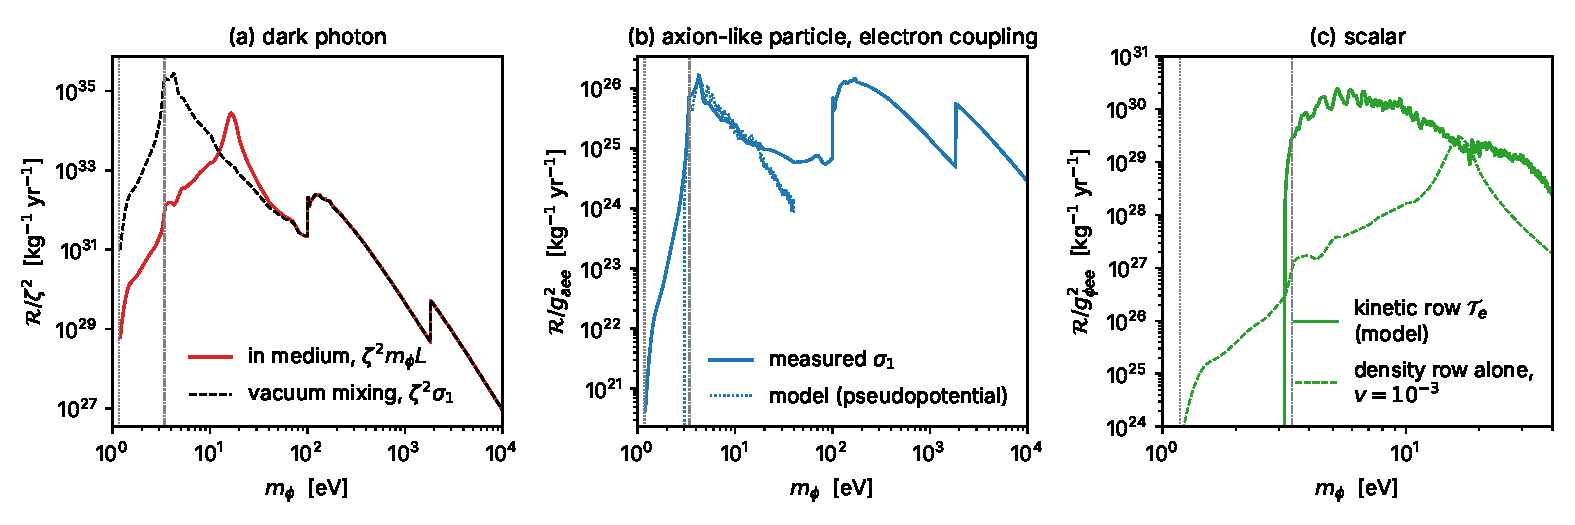
\includegraphics[width=\linewidth]{figures/ch10/fig10_6.pdf}
  \caption{Absorption rates of bosonic dark matter on the electrons of silicon, per kilogram-year and per unit squared coupling, against the boson mass $m_\phi$, with $\rho_\chi = \SI{0.3}{GeV.cm^{-3}}$ and $\rho_T = \SI{2.33}{g.cm^{-3}}$. Measured optical constants of float-zone silicon at \SI{300}{K}~\cite{franta2017temperature} below \SI{40}{eV}, and $\varepsilon$ from the atomic scattering factors of Ref.~\cite{henke1993xray} above, spliced at \SI{40}{eV}. The data are used without transfer to millikelvin temperatures and are wrong within a few tens of meV of the edge (\cref{sec:10.7-edge}). Dotted line: the excitonic edge of cold silicon, \SI{1.1728}{eV} with $\Eg(0) = \SI{1.1692}{eV}$; dash-dotted: the direct gap, \SI{3.4}{eV}. (a) Dark photon: in-medium rate $\zeta^2(\rho_\chi/\rho_T)L$, \cref{eq:10.7-dp} (red), and the vacuum-mixing rate $\zeta^2(\rho_\chi/\rho_T)\sigma_1/m_\phi$ (dashed). The same curve gives the axion-like particle in a field $\vect{B}_0$ with $\zeta \to g_{a\gamma\gamma}B_0/m_\phi$, \cref{eq:10.7-alpB}. (b) Axion-like particle with the electron coupling, \cref{eq:10.7-alp}, from the measured $\sigma_1$ (solid) and from the empirical-pseudopotential model of \cref{sec:4.6} (dotted; independent particles, no spin--orbit coupling, $16^3$ $\vect{k}$ points). (c) Scalar, \cref{eq:10.7-scalar}: kinetic-energy row in the same model, which has pseudo-wavefunctions without core oscillations and its own vertical gap of \SI{3.12}{eV} (solid; histogram of \SI{0.05}{eV} bins, smoothed over \SI{0.25}{eV}); and the screened density row alone at $|\vect{p}_\phi| = 10^{-3}m_\phi$ with the measured loss function (dashed). The model curves show the size and shape of the kinetic and spin responses, not predictions for silicon.}
  \label{fig:10-absorption}
\end{figure}

\begin{workedexample}{Dark-photon absorption at \SI{10}{eV}}\label{we:10-darkphoton}
At \SI{10}{eV} the measured dielectric function of silicon is $\varepsilon = -1.879 + 1.268\,\ii$: the frequency lies above the main interband peaks, where $\varepsilon_1$ has turned negative, and below the plasma frequency, where it turns positive again. Then $|\varepsilon|^2 = 5.139$, $L = \varepsilon_2/|\varepsilon|^2 = 0.2467$ and $\sigma_1 = \omega\varepsilon_2 = \SI{12.68}{eV}$. The in-medium mixing is $\zeta_{\mathrm{eff}}/\zeta = 1/|\varepsilon| = 0.441$, and the rate is suppressed by $1/|\varepsilon|^2 = 0.195$, a factor of 5.1. The photon self-energy is $\Pi_{\mathrm{em}} = m_\phi^2(1 - \varepsilon) = (288 - 127\,\ii)\,\mathrm{eV}^2$, larger than $m_\phi^2 = \SI{100}{eV^2}$.

With $\rho_\chi/m_\phi = \SI{3.0e7}{cm^{-3}}$, \cref{eq:10.7-dp} gives $\mathcal{R} = 1.52\times10^{33}\,\zeta^2$ per kilogram-year, against $7.82\times10^{33}\,\zeta^2$ with the vacuum mixing. Three events in a kilogram-year, the background-free reach, need $\zeta = 4.4\times10^{-17}$; the vacuum mixing would claim $2.0\times10^{-17}$, a reach better by $|\varepsilon| = 2.27$ than the true one. For a halo particle with $v = 10^{-3}$ the transverse and longitudinal rates differ by $v^2[2\Real(1/\varepsilon) - 1] = -1.7\times10^{-6}$, and each differs from \cref{eq:10.7-dp} at the level of $10^{-6}$.
\end{workedexample}

\subsection{Optical data near the silicon edge}\label{sec:10.7-edge}

Optical constants are measured at room temperature or at \SI{77}{K}, and a detector runs at \SI{10}{mK}. Above the direct gap of silicon, \SI{3.4}{eV}, the difference in temperature hardly matters: the transitions are vertical, the bands shift by tens of meV, and $\sigma_1$ changes little. Between the indirect gap and \SI{3.4}{eV} it matters a great deal. There every absorbed photon, and every absorbed dark-matter boson, needs a phonon to supply the crystal momentum $\vect{k}_{\mathrm{c}}$ of the conduction valley (\cref{sec:6.5}). The measured $\sigma_1$ in that window is the phonon-assisted $\omega\varepsilon_2^{\mathrm{PA}}$, second order in the electron--phonon vertex and first order in the phonon occupations, and it depends on temperature at the edge in two ways. At \SI{300}{K} the gap is \SI{1.12}{eV} instead of \SI{1.17}{eV}, and the transverse-acoustic phonon at $\vect{k}_{\mathrm{c}}$ has the occupation 0.97, so that a photon can be absorbed together with a phonon taken from the lattice, from $\Eg - \omega_{\mathrm{TA}}$ up. At \SI{10}{mK} no phonons are present to be absorbed, and the edge of cold silicon lies at $\Eg(0) + \omega_{\mathrm{TA}} - E_x^b = \SI{1.1728}{eV}$ with $\Eg(0) = \SI{1.1692}{eV}$, the excitonic threshold of phonon emission (\cref{sec:6.5}).

The consequence for a rate is direct. The \SI{300}{K} data give $\sigma_1 = 4.9\times10^{-4}$\,eV at \SI{1.15}{eV}, where a cold crystal absorbs nothing, and \cref{fig:10-absorption} inherits the warm edge. The \SI{77}{K} data are closer, but the occupation of the transverse-acoustic phonon is still 0.068 there, and the gap is \SI{1.165}{eV} against \SI{1.169}{eV} at millikelvin temperatures, from the measured temperature dependence of the gap~\cite{alex1996temperature} (\cref{sec:6.3}). Measured $\sigma_1$ near the edge must therefore be transferred to the temperature of the detector before it enters \cref{eq:10.7-dp} or the axion-like rate below. The transfer runs the phonon-assisted formula backward: each branch is separated into its absorption and emission parts, the absorption parts are removed, the emission parts are reweighted from $n_{\vect{Q}\nu} + 1$ to one, and the gap is shifted. Without data resolved by branch the separation is not unique. \Cref{sec:13.5} carries out the transfer and finds that the untransferred \SI{77}{K} data overestimate the millikelvin dark-photon rate of silicon by more than a factor of two within about \SI{20}{meV} of the edge.

\subsection{Axion-like-particle absorption}\label{sec:10.7-alp}

The axion-like particle couples to the electrons through \cref{eq:8.1-alp}, $(g_{aee}/m_e)[(\nabla\phi)\cdot\vect{s}_e + (\partial_t\phi)\mathcal{J}^{\alpha\alpha}_e]$ with the spin current traced over its two indices. For a particle of the halo the spin-density term is negligible. The coefficient of the spin-density term carries $|\vect{p}_\phi|$ instead of $m_\phi$. Without spin--orbit coupling the total spin also commutes with the Hamiltonian, so $\vect{s}_e(\vect{p}_\phi)$ connects different states only at first order in $\vect{p}_\phi$. The spin-density amplitude is then of order $p_\phi^2$, against $m_\phi$ times an electron velocity for the spin current. Only the row $\mathcal{J}_e \equiv \mathcal{J}^{\alpha\alpha}_e(0)$ is left, with $g^\phi_{\mathcal{J}} = g_{aee}m_\phi/m_e$ per unit amplitude, and \cref{eq:8.2-abs} gives $\varGamma = (g_{aee}^2m_\phi/2m_e^2)\,S_{\mathcal{J}\mathcal{J}}(0, m_\phi)$.

The spin current is related to the ordinary current by a spin trace. An electron--hole pair $(c\sigma', v\sigma)$ is created by $\mathcal{J}_e$ with the amplitude $\sum_\alpha v^\alpha_{cv}(S^\alpha)_{\sigma'\sigma}$, with $\vect{v}_{cv} = \langle c|\vect{p}/m_e|v\rangle$, and by the current along a unit vector $\hat{\vect{e}}$ with $\hat{\vect{e}}\cdot\vect{v}_{cv}\,\delta_{\sigma'\sigma}$. Summed over the spins, the spin-current amplitude gives $\sum_{\alpha\beta}v^\alpha_{cv}v^{\beta*}_{cv}\Tr(S^\alpha S^\beta) = |\vect{v}_{cv}|^2/2$, and the current amplitude gives $2|\hat{\vect{e}}\cdot\vect{v}_{cv}|^2$, which in a cubic crystal averages to $2|\vect{v}_{cv}|^2/3$. For independent electrons without spin--orbit coupling, therefore, $S_{\mathcal{J}\mathcal{J}} = \frac34 S_{jj}$, three Cartesian directions times the quarter that \cref{sec:10.5-triplet} found for every spin row. The transverse current response is the conductivity, $S_{jj}(0,\omega) = 2\omega\sigma_1/e^2$ (\cref{sec:4.4,sec:8.2-absorption}), and
\begin{keyresult}[Absorption of an axion-like particle through its electron coupling]
\begin{equation}
  \varGamma = \frac{3\,m_\phi^2}{4\,m_e^2}\,\frac{g_{aee}^2}{e^2}\,\sigma_1(m_\phi) , \qquad
  \mathcal{R} = \frac{\rho_\chi}{\rho_T\,m_\phi}\,\frac{3\,m_\phi^2\,g_{aee}^2}{4\,m_e^2\,e^2}\,\sigma_1(m_\phi) ,
  \label{eq:10.7-alp}
\end{equation}
for independent electrons without spin--orbit coupling~\cites[Eq.~(10)]{hochberg2017absorption}[Eq.~(47)]{mitridate2021dark}. There is no in-medium factor: the rate contains $\sigma_1$ in place of the loss function.
\end{keyresult}
\noindent The spin trace also explains the absence of mixing. A photon-reducible chain needs a proper correlation of $\mathcal{J}_e$ with the charge density, and a single spin operator traced over an unpolarized pair vanishes, $\Tr S^\alpha = 0$, so that $\tilde R_{\mathcal{J}Z} = 0$ (\cref{sec:8.4-mixing}). The parity of the particle says the same: a pseudoscalar cannot mix with the photon of a medium that has neither handedness nor magnetization~\cite[Sect.~III\,B, footnote~5]{mitridate2021dark}. Compared to the dark photon, then, the axion-like particle is not suppressed where the target absorbs light and not enhanced at the plasmon. At equal couplings the ratio of the axion-like rate to the dark-photon rate is $(3m_\phi^2/4m_e^2e^2)|\varepsilon|^2$, which at \SI{10}{eV} is $1.6\times10^{-8}$: the factor $m_\phi^2/m_e^2$ comes from a coupling to spin that a slow electron transmits only through its velocity. \Cref{fig:10-absorption}b shows the rate from the measured $\sigma_1$. The empirical-pseudopotential model of \cref{sec:4.6} gives 0.8 to 1.15 times the measured value between 4 and \SI{18}{eV}, and half of it at \SI{20}{eV}, far above the transitions to which its three form factors were fitted.

\Cref{eq:10.7-alp} uses the measured $\sigma_1$ for a response that differs from the one measured. The current creates electron--hole pairs in the spin singlet, and the spin current in the triplet. With the interaction switched on, the singlet pairs feel both kernels of the Bethe--Salpeter equation and the triplet pairs only the direct one, \cref{eq:10.5-triplet}. The excitonic attraction is common to the singlet and triplet pairs, and the measured edge carries it correctly. The local fields, however, which are the rest of the exchange kernel, act on the singlet pairs alone. In the model of \cref{sec:4.6} they lower the main $\varepsilon_2$ peak of silicon from 41 to 34 and move it up by \SI{60}{meV}. The measured $\sigma_1$ therefore understates the axion-like response near its peak by about a fifth, and by less where the local fields are weak. Spin--orbit coupling is the second caveat. It ties the spin to the orbital motion, the spin trace no longer factorizes, and the factor $\frac34$ acquires corrections set by the spin--orbit splitting over the transition energy, $\Delta_{\mathrm{SO}} = \SI{0.044}{eV}$ in silicon against several eV (\cref{sec:3.3}). In germanium, GaAs and heavier targets the current and spin-current responses must be computed separately.

The photon coupling, $g_{a\gamma\gamma}\phi\,\vect{E}\cdot\vect{B}$ of \cref{sec:1.4}, needs a field to act on. In a static laboratory field $\vect{B}_0$ it reads $g_{a\gamma\gamma}\phi\,\vect{E}\cdot\vect{B}_0 = -g_{a\gamma\gamma}\phi\,(\partial_t\vect{A})\cdot\vect{B}_0$ in the gauge without scalar potential, and after an integration by parts in time it is $\vect{J}_a\cdot\vect{A}$, with a source current along the field,
\begin{equation*}
  \vect{J}_a = g_{a\gamma\gamma}\,(\partial_t\phi)\,\vect{B}_0 ,
\end{equation*}
which oscillates at $m_\phi$ with the wavevector $\vect{p}_\phi$. The medium answers as it answers any current. For a sample much larger than the skin depth $(m_\phi\Imag\sqrt{\varepsilon})^{-1}$ its boundaries do not matter~\cite[footnote~1]{berlin2024absorption}, and at $\vect{p}_\phi \to 0$ the curl of the magnetic field drops out of the Amp\`ere--Maxwell law $\nabla\times\vect{B} = \vect{J} + \partial_t\vect{E}$ of \cref{sec:4.4}, with a relative error of order $p_\phi^2/\omega^2$. The induced current is $\vect{J}_{\mathrm{ind}} = \sigma_{\mathrm{cond}}\cdot\vect{E}$, with the conductivity tensor, so that $0 = \vect{J}_a + \sigma_{\mathrm{cond}}\cdot\vect{E} - \ii\omega\vect{E} = \vect{J}_a - \ii\omega\,\varepsilon\cdot\vect{E}$, by \cref{eq:4.4-sigma}. With the amplitude $\phi_0$ of $\phi = \Real(\phi_0\ee^{-\ii m_\phi t})$, $\vect{J}_a$ has the amplitude $-\ii m_\phi g_{a\gamma\gamma}\phi_0\vect{B}_0$, and the field is
\begin{equation*}
  \vect{E} = \frac{1}{\ii\omega}\,\varepsilon^{-1}\cdot\vect{J}_a = -g_{a\gamma\gamma}\,\phi_0\,\varepsilon^{-1}(m_\phi)\cdot\vect{B}_0 .
\end{equation*}
The power that this field dissipates per unit volume, averaged over a period, is $\frac12\Real(\vect{J}^*_{\mathrm{ind}}\cdot\vect{E}) = \frac{\omega}{2}\vect{E}^\dagger\cdot\varepsilon''\cdot\vect{E}$, with $\varepsilon'' = (\varepsilon - \varepsilon^\dagger)/2\ii$ the absorptive part of the tensor. Since $(\varepsilon^{-1})^\dagger(\varepsilon - \varepsilon^\dagger)\varepsilon^{-1} = (\varepsilon^{-1})^\dagger - \varepsilon^{-1}$, the power is $\frac{\omega}{2}g_{a\gamma\gamma}^2|\phi_0|^2\,\vect{B}_0\cdot\Imag[-\varepsilon^{-1}]\cdot\vect{B}_0$, where $\Imag[-\varepsilon^{-1}]$ denotes the absorptive part of $-\varepsilon^{-1}$. The number density of the field is its energy density $\frac12m_\phi^2|\phi_0|^2$ over $m_\phi$. Division of the power by the number density and by the energy $\omega$ of one quantum gives
\begin{keyresult}[Absorption of an axion-like particle in a static field]
\begin{equation}
  \varGamma = \frac{g_{a\gamma\gamma}^2B_0^2}{m_\phi}\;\hat{\vect{B}}_0\cdot\Imag\bigl[-\varepsilon^{-1}(m_\phi)\bigr]\cdot\hat{\vect{B}}_0 , \qquad
  \mathcal{R} = \frac{\rho_\chi}{\rho_T}\,\frac{g_{a\gamma\gamma}^2B_0^2}{m_\phi^2}\;\hat{\vect{B}}_0\cdot\Imag\bigl[-\varepsilon^{-1}\bigr]\cdot\hat{\vect{B}}_0 ,
  \label{eq:10.7-alpB}
\end{equation}
the inverse dielectric tensor projected on the direction of the field~\cite[Eqs.~(6) and (7)]{berlin2024absorption}. In a cubic crystal the projection is the loss function $L(m_\phi)$, and the rate equals the dark-photon rate with $\zeta = g_{a\gamma\gamma}B_0/m_\phi$.
\end{keyresult}
\noindent \Cref{fig:10-absorption}a gives the rate of the axion-like particle in a field for silicon with that substitution. A field of \SI{10}{T} is $B_0 = \SI{1953}{eV^2}$ in the units of \cref{app:A.2}, and with $g_{a\gamma\gamma} = \SI{e-10}{GeV^{-1}}$ the equivalent mixing at \SI{10}{eV} is $2.0\times10^{-17}$, or 0.58 events per kilogram-year in silicon. The field also acts on the target, through the Zeeman and orbital energies, but $\mu_{\mathrm{B}}B_0 = \SI{0.58}{meV}$ at \SI{10}{T} is negligible against electronic energies, and the derivation never used the symmetry of $\varepsilon$, only its absorptive part. The two couplings of the axion-like particle add without interference: the cross term needs a correlation of the spin current with the charge current, and this correlation vanishes without spin--orbit coupling for the same reason as $\tilde R_{\mathcal{J}Z}$.

In a crystal of lower symmetry the projection of the inverse is not the inverse of the projection. For a uniaxial crystal with the field at an angle $\theta$ to the optic axis, $\hat{\vect{B}}_0\cdot\varepsilon^{-1}\cdot\hat{\vect{B}}_0 = \cos^2\theta/\varepsilon_\parallel + \sin^2\theta/\varepsilon_\perp$, while the dielectric function along the field is $\varepsilon_{BB} = \cos^2\theta\,\varepsilon_\parallel + \sin^2\theta\,\varepsilon_\perp$, and
\begin{equation}
  \hat{\vect{B}}_0\cdot\varepsilon^{-1}\cdot\hat{\vect{B}}_0 - \frac{1}{\varepsilon_{BB}} = \frac{\cos^2\theta\,\sin^2\theta\,(\varepsilon_\parallel - \varepsilon_\perp)^2}{\varepsilon_\parallel\,\varepsilon_\perp\,\varepsilon_{BB}} .
  \label{eq:10.7-aniso}
\end{equation}
The difference is second order in the anisotropy and vanishes on the principal axes. Near a longitudinal resonance of one axis it is not small, because $1/\varepsilon_\parallel$ or $1/\varepsilon_\perp$ is large there while $\varepsilon_{BB}$ is not near zero. The isotropic formula with the dielectric function along the field then misses the resonance, and \cref{eq:10.7-alpB} keeps it.

\begin{limitbox}[Absorption with in-medium mixing][lim:10.7a]
Dark photon: $\mathcal{R} = (\rho_\chi/\rho_T m_\phi)\,\zeta_{\mathrm{eff}}^2\sigma_1(m_\phi)$, $\zeta_{\mathrm{eff}}^2 = \zeta^2m_\phi^4/|m_\phi^2 - \Pi_{\mathrm{em}}|^2$~\cite[Eqs.~(6) and (7)]{hochberg2017absorption}, which for $m_\phi^2 \gg |\Pi_{\mathrm{em}}|$ reduces to the vacuum mixing, $\varGamma = \zeta^2\sigma_1$~\cite[Eq.~(20)]{an2015direct}. Axion-like particle in a field: $\varGamma = (g_{a\gamma\gamma}B_0)^2\Imag[-1/\varepsilon(m_\phi)]/m_\phi$ for an isotropic target~\cite[Eq.~(7)]{berlin2024absorption}.
\par\smallskip
{\centering
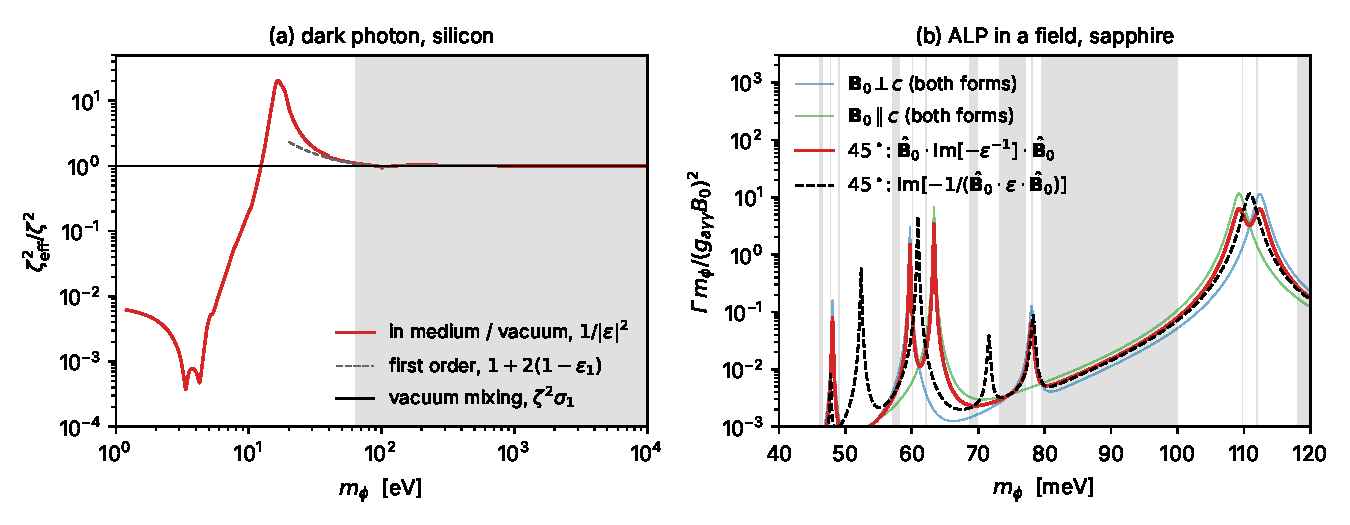
\includegraphics[width=\linewidth]{figures/ch10/limit10_7a.pdf}
\captionof{figure}{(a) Dark photon in silicon: the in-medium rate over the vacuum-mixing rate, $\zeta_{\mathrm{eff}}^2/\zeta^2 = 1/|\varepsilon(m_\phi)|^2$ (red), against the vacuum-mixing limit (black). Measured $\varepsilon$ at \SI{300}{K} below \SI{40}{eV}~\cite{franta2017temperature} and from atomic scattering factors above~\cite{henke1993xray}. Gray: masses where $1/|\varepsilon|^2$ is within \SI{10}{\percent} of one, all masses above \SI{63}{eV}. A halo momentum $|\vect{p}_\phi| = 10^{-3}m_\phi$ changes the transverse and longitudinal rates by $10^{-6}$, invisible here. (b) Axion-like particle in a field at \SI{45}{\degree} to the optic axis of sapphire: the rate of \cref{eq:10.7-alpB}, $\hat{\vect{B}}_0\cdot\Imag[-\varepsilon^{-1}]\cdot\hat{\vect{B}}_0$ (red), against the isotropic formula evaluated with the dielectric function along the field, $\Imag[-1/\varepsilon_{BB}]$ (dashed), and the two principal axes, where both forms agree (thin). Phonon dielectric functions of sapphire in the damped factorized form $\varepsilon = \varepsilon_\infty\prod_\nu(\omega_{\mathrm{L}\nu}^2 - \omega^2 - \ii\omega\gamma_{\mathrm{L}\nu})/(\omega_{\mathrm{T}\nu}^2 - \omega^2 - \ii\omega\gamma_{\mathrm{T}\nu})$ with $\varepsilon_\infty = 3.2$ and the frequencies and \SI{77}{K} widths of Ref.~\cite[Eq.~(37), Tables~I and II]{griffin2018directional} (ordinary ray, longitudinal 112.4, 78.0, 59.7 and \SI{48.1}{meV} with widths 1.98, 0.55, 0.17 and \SI{0.17}{meV}, transverse 78.6, 70.5, 54.4 and \SI{47.7}{meV} with widths 0.47, 0.40, 0.19 and \SI{0.17}{meV}; extraordinary ray, longitudinal 109.2 and \SI{63.3}{meV} with widths 1.98 and \SI{0.17}{meV}, transverse 72.2 and \SI{49.3}{meV} with widths 0.40 and \SI{0.19}{meV}), with the widths of the extraordinary ray borrowed from the ordinary modes. Gray: masses where the two forms agree within \SI{10}{\percent}. Silicon is cubic, and in silicon the two forms coincide.}\label{fig:10-abs-limit}
\par}
\smallskip
Below \SI{63}{eV} the medium changes the dark-photon rate of silicon by factors from $4\times10^{-4}$ to 20, and in an anisotropic crystal with the field off its principal axes the isotropic formula misses the longitudinal resonances of each axis by up to a factor of several hundred.
\end{limitbox}

\subsection{Scalar absorption and the kinetic-energy row}\label{sec:10.7-scalar}

A scalar coupled to $\bar\psi\psi$ acts on the target through \cref{eq:8.1-scalar}, $-g_{\phi ee}\phi\,[n_e(\vect{p}_\phi) - \mathcal{T}_e(\vect{p}_\phi)/m_e]$: on the number of electrons and, at next order in $1/m_e$, on their kinetic energy. For scattering the density row dominates. For absorption at $|\vect{p}_\phi| \approx 10^{-3}m_\phi$ the order is reversed: the density row connects different states only at first order in $\vect{p}_\phi$ and is suppressed by $v^2$ in the rate, while the kinetic row is not (\cref{sec:8.1-absorption}).

\Cref{sec:8.4-mixing} found that the scalar mixes with the photon through the proper correlations $\tilde R_{n_eZ}$ and $\tilde R_{\mathcal{T}_eZ}$ of its two rows with the charge. The correlation $\tilde R_{n_eZ}$ is the density response, of order $p_\phi^2$. For $\tilde R_{\mathcal{T}_eZ}$, expand in $\vect{p}_\phi$: $\tilde R_{\mathcal{T}_en_e}(\vect{p}_\phi,\omega) = \vect{p}_\phi\cdot\vect{F}(\omega) + O(p_\phi^2)$, where $\vect{F}$ is a vector built from the crystal alone. It must be invariant under every operation of the point group, and an invariant vector exists only in a polar group, one that leaves some direction fixed under every operation. Crystals with a polar group are pyroelectric: they carry a spontaneous electric polarization along that direction. Silicon ($O_h$), GaAs ($T_d$) and sapphire ($D_{3d}$) have no invariant vector, and in them $\tilde R_{\mathcal{T}_en_e} = O(p_\phi^2)$. The photon-reducible part, $\tilde R_{\mathcal{T}_eZ}\,v_{\mathrm{C}}(p_\phi)\,\varepsilon^{-1}\,\tilde R_{Z\mathcal{T}_e}$, is then of order $p_\phi^4\cdot e^2/p_\phi^2 = e^2p_\phi^2$ and vanishes with the density row. In a polar crystal, such as wurtzite GaN or ZnO, $\vect{F} \ne 0$ and the mixing survives at $\vect{p}_\phi \to 0$ as a term $(e^2/\omega^2)\,\hat{\vect{p}}_\phi\cdot\tilde R_{\mathcal{T}_e\vect{j}}\,\varepsilon^{-1}\,\tilde R_{\vect{j}\mathcal{T}_e}\cdot\hat{\vect{p}}_\phi$, with $n_e = \vect{p}_\phi\cdot\vect{j}_e/\omega$ on the energy shell (\cref{eq:4.3-continuity}). With only the kinetic row kept, and with $g^\phi_{\mathcal{T}_e} = g_{\phi ee}/m_e$ in \cref{eq:8.2-abs},
\begin{keyresult}[Scalar absorption]
\begin{equation}
  \varGamma = -\frac{g_{\phi ee}^2}{m_\phi\,m_e^2}\,\Imag R_{\mathcal{T}\mathcal{T}}(0, m_\phi) = \frac{g_{\phi ee}^2}{2\,m_\phi\,m_e^2}\,S_{\mathcal{T}\mathcal{T}}(0, m_\phi) ,
  \label{eq:10.7-scalar}
\end{equation}
with $R_{\mathcal{T}\mathcal{T}}$ the response of the kinetic-energy row $\mathcal{T}_e(0) = \sum_jp_j^2/2m_e$ at $T = 0$, for every crystal whose point group has no polar vector, up to corrections of order $v^2$ from the other rows~\cite[Eqs.~(55) and (56)]{mitridate2021dark}. The response is unscreened, and no optical measurement gives it.
\end{keyresult}
\noindent In the notation of Mitridate and collaborators the row is $\bar v^2 = \mathcal{T}_e/m_e$ and the coupling $d_{\phi ee}$, with $g_{\phi ee} = d_{\phi ee}\sqrt{4\pi}\,m_e/M_{\mathrm{Pl}}$ (\cref{sec:1.4}). For independent electrons the response is a joint density of states weighted by the kinetic matrix elements,
\begin{equation}
  S^0_{\mathcal{T}\mathcal{T}}(0,\omega) = \frac{4\pi}{\Vol}\sum_{cv\vect{k}}\bigl|\langle c\vect{k}|\mathcal{T}_e|v\vect{k}\rangle\bigr|^2\,\delta(\omega - \varepsilon_{c\vect{k}} + \varepsilon_{v\vect{k}}) ,
  \label{eq:10.7-S0}
\end{equation}
spin summed, with the one-electron element $\langle c|p^2/2m_e|v\rangle = \sum_m\vect{p}_{cm}\cdot\vect{p}_{mv}/2m_e$, a sum over all bands, the core included. Since $c$ and $v$ are eigenstates of $p^2/2m_e + V$ with different energies, the element is also $-\langle c|V|v\rangle$: the kinetic row measures the matrix elements of the crystal potential itself. Those are largest where the potential is deep, near the nuclei, and there a pseudo-wavefunction is smooth where the true state oscillates. The rate is therefore sensitive to the core region in a way that the conductivity is not, and a calculation needs the all-electron states or their reconstruction from a projector-augmented-wave basis.

The kinetic row also follows a different selection rule. It is even under inversion, while the momentum is odd. At $\mathrm{\Gamma}$ the top valence states of silicon and the lowest conduction states have opposite parity, and the opposite parity makes the direct transition at \SI{3.4}{eV} allowed for light. For the scalar the direct transition is forbidden: in the model of \cref{sec:4.6} the kinetic matrix element between them vanishes at $\mathrm{\Gamma}$ to machine precision, while the momentum element does not, and the scalar spectrum rises from the vertical gap more slowly than $\varepsilon_2$. Below the direct gap the scalar, like the dark photon, is absorbed only with a phonon, and its rate there needs the phonon-assisted kinetic row.

The kinetic row has a sum rule of its own. The first-moment identity \cref{eq:4.3-firstmoment} at $\vect{q} = 0$ gives $\int_0^\infty\dd\omega\,\omega\,S_{\mathcal{T}\mathcal{T}} = (\pi/\Vol)\langle[[\mathcal{T}_e, H], \mathcal{T}_e]\rangle$ at $T = 0$. Take electrons that move independently in a local one-body potential, $H = \sum_j[p_j^2/2m_e + V(\vect{r}_j)]$. With $\mathcal{T}_e = H - \sum_jV(\vect{r}_j)$ written in the outer commutator, the part with $H$ has zero expectation value in an eigenstate, and what remains is $-\langle[[\mathcal{T}_e, V], V]\rangle$. For one electron $[p^2, V] = -\ii(\vect{p}\cdot\nabla V + \nabla V\cdot\vect{p})$, and a second commutator with $V$ leaves $[[p^2, V], V] = -2|\nabla V|^2$. Per electron, then, $\frac12\langle[[\mathcal{T}_e, H], \mathcal{T}_e]\rangle = \langle|\nabla V|^2\rangle/2m_e$, and
\begin{equation}
  \int_0^\infty\dd\omega\;\omega\,S_{\mathcal{T}\mathcal{T}}(0,\omega) = \frac{\pi\,\nd_e}{m_e}\,\bigl\langle|\nabla V|^2\bigr\rangle ,
  \label{eq:10.7-sumrule}
\end{equation}
with the average taken per electron. Compared to the $f$-sum rule \cref{eq:4.3-fsum}, which has $\pi\nd_eq^2/m_e$, the squared momentum kick $q^2$ is replaced by the mean squared force on an electron. For the absorption rate the sum rule fixes $\int\dd m_\phi\,m_\phi^2\varGamma = \pi g_{\phi ee}^2\nd_e\langle|\nabla V|^2\rangle/2m_e^3$.

The conditions are restrictive: a potential that is local and one-body, and a mean squared force that is finite. A nonlocal pseudopotential keeps the identity in the form $-\langle[[\mathcal{T}_e,V_{\mathrm{NL}}],V_{\mathrm{NL}}]\rangle$, but the double commutator is then no longer $\langle|\nabla V|^2\rangle$, just as nonlocality changes the $f$-sum rule (\cref{eq:4.3-fsumNL}). The Coulomb repulsion between the electrons turns $\langle|\nabla V|^2\rangle$ into the mean squared total force on an electron, a two-body and three-body average. The decisive failure is the Coulomb potential of a nucleus, which makes the force diverge: $|\nabla V|^2 = Z^2\alpha^2/r^4$, and an $s$ state, with a finite density at the nucleus, gives $\int r^2\dd r/r^4 = \infty$. The valence states of silicon have s character inside the core, where they oscillate to stay orthogonal to the $1s$ and $2s$ states, so for the real crystal the right-hand side of \cref{eq:10.7-sumrule} is infinite. The spectrum of the kinetic row has a tail that decays too slowly for its first moment to converge, and \cref{eq:10.7-sumrule} cannot normalize it as the $f$-sum rule normalizes the density response. The sum rule does provide a check of a calculation within its own model, for a local and regular potential such as an empirical pseudopotential, or the valence block of a calculation whose potential is regular.

\begin{limitbox}[Scalar absorption through the kinetic-energy row][lim:10.7b]
$\varGamma = -(g_{\phi ee}^2/m_\phi m_e^2)\Imag R_{\mathcal{T}\mathcal{T}}(0, m_\phi)$, from the kinetic-energy term of the nonrelativistic scalar coupling~\cite[Eqs.~(18) and (56)]{mitridate2021dark}; its energy-weighted integral is \cref{eq:10.7-sumrule} for a local, regular one-body potential.
\par\smallskip
{\centering
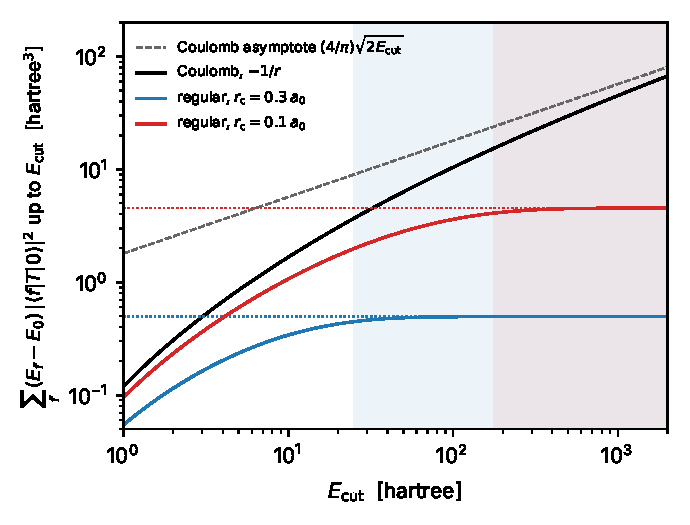
\includegraphics[width=0.66\linewidth]{figures/ch10/limit10_7b.pdf}
\captionof{figure}{Energy-weighted spectrum of the kinetic row, $\sum_f(E_f - E_0)|\langle f|p^2/2m_e|0\rangle|^2$ over final states up to an excitation energy $E_{\mathrm{cut}}$, for one electron in its ground state (atomic units), against $E_{\mathrm{cut}}$. Black: Coulomb potential $-1/r$, hydrogen; dashed, its asymptote $(4/\pi)\sqrt{2E_{\mathrm{cut}}}$, from the plane-wave limit of the continuum states. Blue and red: the regular potentials $-1/(r^2 + r_{\mathrm{c}}^2)^{1/2}$ with $r_{\mathrm{c}} = 0.3$ and $0.1\,a_0$; dotted, their sum rules $\langle|\nabla V|^2\rangle/2$, \cref{eq:10.7-sumrule}. Shaded: $E_{\mathrm{cut}}$ above which each regular spectrum holds \SI{90}{\percent} of its sum rule, 25 and \SI{176}{hartree}. Only s states contribute, since the kinetic energy conserves angular momentum. Radial equation on a uniform grid of \SI{0.004}{a_0} in a box of \SI{30}{a_0}; on the full grid the spectral sum and the double commutator agree to six digits.}\label{fig:10-scalar-limit}
\par}
\smallskip
For the Coulomb potential of a nucleus the energy-weighted spectrum grows as $E_{\mathrm{cut}}^{1/2}$ without limit, so the sum rule exists only for regular potentials, and its value grows as the core radius shrinks.
\end{limitbox}

The empirical-pseudopotential model of \cref{sec:4.6} is local and regular, and it satisfies \cref{eq:10.7-sumrule} exactly within its basis of 113 plane waves. On a grid of $16^3$ $\vect{k}$ points the spectral first moment and the double commutator agree to six digits, at $\langle|\nabla V|^2\rangle/2m_e = 1.30\times10^3\,\mathrm{eV}^3$ per valence electron. Only \SI{2}{\percent} of the first moment lies below \SI{10}{eV} and \SI{41}{\percent} below \SI{40}{eV}. Even in a model with a regular potential, then, the sum rule is carried by transitions far above the masses that matter, and it constrains the low-energy spectrum only weakly. \Cref{fig:10-absorption}c shows the model's scalar rate in silicon: $9.8\times10^{29}\,g_{\phi ee}^2$ per kilogram-year at \SI{10}{eV}, four orders of magnitude above the axion-like rate at equal coupling. The comparison with the electron's momentum makes the ratio of the scalar to the axion-like rate plausible. The kinetic matrix elements are a few eV, so $\mathcal{T}_e/m_e \sim 10^{-5}$, while the axion-like amplitude carries $m_\phi/m_e$ times an electron velocity, $\sim 10^{-7}$. The absolute value of the model curve is not a prediction, for the reason given above, and an all-electron response fixes it.

The dashed curve of \cref{fig:10-absorption}c is the density row alone, screened with the measured loss function, $(g_{\phi ee}^2/2m_\phi)(2p_\phi^2/e^2)L$ at $|\vect{p}_\phi| = 10^{-3}m_\phi$. It is one of the terms of order $v^2$ in \cref{eq:10.7-scalar}. At \SI{5}{eV} it is $3\times10^{-3}$ of the model's kinetic rate and at \SI{10}{eV} $2\times10^{-2}$. Near the plasma frequency, however, the density row is enhanced by the same factor $1/|\varepsilon|^2$ that enhances the dark photon, and between 16 and \SI{18}{eV} it is as large as the model's kinetic rate. The all-electron calculation of Mitridate and collaborators finds the kinetic term dominant in silicon and germanium~\cite[Fig.~1 and Sect.~IV]{mitridate2021dark}; its kinetic matrix elements include the core oscillations that our model lacks. The other terms of order $v^2$, the cross term between the rows and the mixing through $\tilde R_{\mathcal{T}_eZ}$, are of the same size as the density row and have not been computed. Within a few eV of the plasma frequency the margin by which \cref{eq:10.7-scalar} holds is therefore open, and it is fixed by the same all-electron calculation, extended to order $p_\phi^2$.

\section{Two-insertion processes}\label{sec:10.8}

A dark photon of \SI{100}{keV} that meets an electron in silicon is more likely to scatter off it than to be absorbed. It leaves as an ordinary photon of \SI{91.8}{keV}, and the electron recoils with the remaining \SI{8.2}{keV}. This is dark Compton scattering, and above about \SI{55}{keV} it is the main way a silicon detector registers a dark photon. Its amplitude carries two insertions of a field: one of the dark photon and one of the photon. A complex scalar that couples quadratically to the electrons, through $\phi^\dagger\phi$, is a second example. It cannot be absorbed singly, since the coupling destroys a particle only together with an antiparticle, and the target absorbs the pair, the energy $2m_\phi$ and the momentum of both. Each process asks the crystal for more than the single row of \cref{sec:10.7}.

\subsection{Second-order transition operator}\label{sec:10.8-rate}

To second order in the interaction $H' = H_{\mathrm{int}}$, the Lippmann--Schwinger series \cref{eq:2.4-LS} gives $T_{fi} = H'_{fi} + \sum_mH'_{fm}H'_{mi}/(E_i - E_m + \ii0^+)$, and the rate is $2\pi|T_{fi}|^2\delta(E_f - E_i)$ (\cref{eq:2.4-golden2}). A field can enter $T_{fi}$ twice in two ways. In the first, one term of $H_{\mathrm{int}}$ is already quadratic in the field and linear in a target operator, so that both insertions sit at one vertex. The first-order term of $T$ then removes two quanta at once, and the target answers with one of its rows $O_a$ at the total momentum and energy of the pair. The rate needs only the response matrix $S_{ab}$ of \cref{eq:8.2-rate}. In the second way, each insertion comes with its own target operator, and the second-order term of $T$ joins them through the target propagator. With insertions $a$ and $b$ that bring $(\vect{k}_1, \omega_1)$ and $(\vect{k}_2, \omega_2)$, the target sees the effective operator
\begin{equation}
  T^{(2)}_{ab} = O_b(\vect{k}_2)\,\frac{1}{E_i + \omega_1 - H_0 + \ii0^+}\,O_a(\vect{k}_1) + O_a(\vect{k}_1)\,\frac{1}{E_i + \omega_2 - H_0 + \ii0^+}\,O_b(\vect{k}_2) ,
  \label{eq:10.8-T2}
\end{equation}
the two time orderings of \cref{eq:2.4-orderings}, and the rate is the response of $T^{(2)}_{ab}$, a four-point function of the target operators, at $(\vect{k}_1 + \vect{k}_2, \omega_1 + \omega_2)$. When neither denominator can vanish, because $\omega_1$ and $\omega_2$ lie below every excitation that $O_a$ and $O_b$ reach, $T^{(2)}_{ab}$ is to leading order a static polarizability of the target, and the four-point function collapses to a two-point function. A vector field coupled to the electron current brings a contact term of its own, the seagull $e^2\vect{A}^2/2m_e$ of the electron Hamiltonian. When the frequencies lie far above the binding energies of the electrons, the second-order terms are small against it, and the seagull alone gives the Thomson limit. Dark Compton scattering is this case (\cref{sec:10.8-compton}). A coupling that has both a contact term and two linear ones gives amplitudes of both kinds, and their interference needs a three-point response of the target, linear in a quadratic response function (\cref{sec:10.8-open}).

\subsection{Pair absorption}\label{sec:10.8-pair}

Take a complex scalar $\phi$ of mass $m_\phi$, whose particles and antiparticles are equally abundant, each with the number density $\rho_\chi/2m_\phi$. Bauer, Perez-Soler and Shergold write its lowest couplings to electrons, in Hamiltonian form, as~\cite[Eq.~(3)]{bauer2026dark}
\begin{equation}
  H_{\mathrm{int}} = \int\dd^3x\,\Bigl[m_e\,\phi^\dagger\phi\;\bar\psi\bigl(G_{\mathrm{S}} + \ii G_{\mathrm{P}}\gamma^5\bigr)\psi
  + \ii\bigl(\phi^\dagger\overleftrightarrow{\partial}_{\!\mu}\phi\bigr)\,\bar\psi\gamma^\mu\bigl(G_{\mathrm{V}} + G_{\mathrm{A}}\gamma^5\bigr)\psi\Bigr] ,
  \label{eq:10.8-Hpair}
\end{equation}
with $\phi^\dagger\overleftrightarrow{\partial}_{\!\mu}\phi = \phi^\dagger\partial_\mu\phi - (\partial_\mu\phi^\dagger)\phi$ and four real couplings of dimension eV$^{-2}$, for scalar, pseudoscalar, vector and axial-vector electron bilinears. They are dimension-six operators, of order $\Lambda_{\mathrm{NP}}^{-2}$ for a new-physics scale $\Lambda_{\mathrm{NP}}$, and we quote rates at $G = G_{\mathrm{F}}$, the Fermi constant. To first order in the couplings the interaction Hamiltonian is minus the interaction Lagrangian, derivative terms included. Each operator is quadratic in $\phi$ and linear in the electrons, so pair absorption is a contact process of the first kind.

\emph{The rate.} Quantize $\phi$ in the box. The field operator removes a particle of momentum $\vect{p}$ with the factor $\ee^{\ii\vect{p}\cdot\vect{x} - \ii E t}/\sqrt{2E\Vol}$ and $\phi^\dagger$ removes an antiparticle of momentum $\bar{\vect{p}}$ with $\ee^{\ii\bar{\vect{p}}\cdot\vect{x} - \ii\bar Et}/\sqrt{2\bar E\Vol}$, with $E$ and $\bar E$ their energies. Removing both from $\phi^\dagger\phi$ leaves the plane wave $\ee^{\ii(\vect{p} + \bar{\vect{p}})\cdot\vect{x}}/(\Vol\sqrt{4E\bar E})$. In $\ii\phi^\dagger\overleftrightarrow{\partial}_{\!\mu}\phi$ the derivatives bring down $-\ii p_\mu$ and $-\ii\bar p_\mu$ with opposite signs, and the same plane wave comes with the factor $(p - \bar p)_\mu$. Every operator of \cref{eq:10.8-Hpair} therefore acts on the target as a row at the total momentum of the pair, $\vect{q} = \vect{p} + \bar{\vect{p}}$, with a coefficient $g^{\phi\phi}_a$ per unit pair amplitude. The coefficients are $m_eG_{\mathrm{S}}$ and $m_eG_{\mathrm{P}}$ against the bilinears $\bar\psi\psi$ and $\bar\psi\ii\gamma^5\psi$, and $G_{\mathrm{V}}(p - \bar p)^\mu$ and $G_{\mathrm{A}}(p - \bar p)^\mu$ against the vector and axial currents. The golden rule, summed over final states, turns $\sum_f2\pi|\langle f|O_b(\vect{q})|i\rangle|^2\delta(\omega - E_f + E_i)$ into $\Vol S_{bb}(\vect{q}, \omega)$, as in \cref{eq:8.2-abs}, and one pair in the box is absorbed at the rate $\sum_{ab}g^{\phi\phi*}_a g^{\phi\phi}_bS_{ab}/(4E\bar E\Vol)$. The box holds $\Vol^2$ times $(\rho_\chi/2m_\phi)^2$ pairs, distributed over the two velocities with the laboratory distribution $f_\chi$ of \cref{sec:1.2}. The number of pairs absorbed per unit time and volume is
\begin{equation}
  \frac{\varGamma_{\mathrm{pair}}}{\Vol} = \Bigl(\frac{\rho_\chi}{2m_\phi}\Bigr)^2\int\dd^3v\,\dd^3\bar v\,f_\chi(\vect{v})f_\chi(\bar{\vect{v}})\,
  \frac{\sum_{ab}g^{\phi\phi*}_a g^{\phi\phi}_b\,S_{ab}(\vect{p} + \bar{\vect{p}},\,E + \bar E)}{4E\bar E} ,
  \label{eq:10.8-pair}
\end{equation}
with $\vect{p} = m_\phi\vect{v}$, $\bar{\vect{p}} = m_\phi\bar{\vect{v}}$ and $E + \bar E = 2m_\phi + K_{\mathrm{pair}}$, where $K_{\mathrm{pair}} = \frac12m_\phi(v^2 + \bar v^2)$ is the kinetic energy of the pair. The event rate per unit target mass is $\varGamma_{\mathrm{pair}}/(\Vol\rho_T)$. This is the golden rule and phase-space measure of Bauer and collaborators~\cite[Eqs.~(5) and (7)]{bauer2026dark} with $S_{ab}$ in place of a single atomic transition. Their truncated Gaussian momentum distribution of each species~\cite[Eq.~(8)]{bauer2026dark}, written per degree of freedom, integrates to the number density $\rho_\chi/2m_\phi$ used here, so their rates equal ours at the same density. Their rates assume $\rho_\chi = \SI{0.39}{GeV.cm^{-3}}$ and scale as $\rho_\chi^2$, so they are larger than at the \SI{0.3}{GeV.cm^{-3}} of \cref{sec:1.2} by $(0.39/0.3)^2 = 1.69$.

The response is sampled close to a single point. The total momentum is at most $2m_\phi v_{\mathrm{max}} = 5.3\times10^{-3}\,m_\phi$, and the pair's kinetic energy has the mean $\bar K_{\mathrm{pair}} = m_\phi\langle v^2\rangle = 1.60\times10^{-6}\,m_\phi$ in the laboratory, for the halo of \cref{sec:1.2} ($\langle v^2\rangle^{1/2} = \SI{379}{km/s}$), with a spread of half that. For an electronic transition at $2m_\phi = \SI{10}{eV}$ the momentum times the lattice constant is $qa < 10^{-4}$. Wherever $S_{ab}$ is smooth on the scale $\bar K_{\mathrm{pair}}$ in energy, it can be taken at $(\vect{0}, 2m_\phi)$, and
\begin{equation}
  \frac{\varGamma_{\mathrm{pair}}}{\Vol} = \Bigl(\frac{\rho_\chi}{2m_\phi}\Bigr)^2\,\frac{\sum_{ab}\langle g^{\phi\phi*}_a g^{\phi\phi}_b\rangle\,S_{ab}(0, 2m_\phi)}{4m_\phi^2} ,
  \label{eq:10.8-contact}
\end{equation}
with the average over the two velocities left only on the coefficients. Pair absorption is single absorption at the energy $2m_\phi$, with a tensor of coefficients that may depend on the velocities. Which rows the four couplings reach, and with what coefficients, follows from the non-relativistic reduction of the electron bilinears, which \cref{sec:1.4,sec:8.1-absorption} have done for linear couplings. The reduction does not care whether the field multiplying a bilinear is $\phi$ or $\phi^\dagger\phi$.

\emph{Scalar.} By \cref{eq:8.1-scalar}, $\bar\psi\psi$ is $n_e - \mathcal{T}_e/m_e$ at low energy. The density row connects different states only at order $q$, and the kinetic row survives at $\vect{q} = 0$, as for a single scalar (\cref{sec:10.7-scalar}). With $g^{\phi\phi} = m_eG_{\mathrm{S}}$ against $\mathcal{T}_e/m_e$, \cref{eq:10.8-contact} gives $(\rho_\chi/2m_\phi)^2G_{\mathrm{S}}^2S_{\mathcal{T}\mathcal{T}}(0, 2m_\phi)/4m_\phi^2$. Compare it with \cref{eq:10.7-scalar} for a scalar of mass $2m_\phi$ and coupling $g_{\phi ee}$, absorbed at the rate $g_{\phi ee}^2S_{\mathcal{T}\mathcal{T}}(0, 2m_\phi)/(4m_\phi m_e^2)$ per particle. The pair rate per unit volume equals the rate of a scalar of mass $2m_\phi$ at the number density $\rho_\chi/2m_\phi$ when
\begin{equation}
  g_{\phi ee}^2 \;\to\; g_{\mathrm{eff}}^2 = \frac{\rho_\chi}{2m_\phi}\,\frac{m_e^2G_{\mathrm{S}}^2}{m_\phi} .
  \label{eq:10.8-geff}
\end{equation}
The rate per unit volume grows as $\rho_\chi^2/m_\phi^4$ at fixed response, and this is what makes pair absorption interesting at small masses.

\emph{Pseudoscalar.} The non-relativistic form of $\bar\psi\ii\gamma^5\psi$ times a field is \cref{eq:1.4-alp}, with $g_{aee}\phi$ replaced by $m_eG_{\mathrm{P}}\phi^\dagger\phi$. It has two terms. The spin-density term carries the gradient of the field, which on the pair is $\ii\vect{q}$, and is negligible. The spin-current term carries its time derivative, which on the pair is $-\ii(E + \bar E) \simeq -2\ii m_\phi$, not the momentum. The pseudoscalar pair is therefore absorbed through the axioelectric row $\mathcal{J}_e$ of \cref{sec:10.7-alp}, with the coefficient $2m_\phi G_{\mathrm{P}}$ in place of $g_{aee}m_\phi/m_e$, and without any velocity suppression. With $S_{\mathcal{J}\mathcal{J}} = \frac34S_{jj}$ and $S_{jj}(0, \omega) = 2\omega\sigma_1/e^2$ (\cref{sec:10.7-alp}),
\begin{equation}
  \frac{\varGamma_{\mathrm{pair}}}{\Vol} = \Bigl(\frac{\rho_\chi}{2m_\phi}\Bigr)^2G_{\mathrm{P}}^2\,S_{\mathcal{J}\mathcal{J}}(0, 2m_\phi) = \Bigl(\frac{\rho_\chi}{2m_\phi}\Bigr)^2\,\frac{3m_\phi\,G_{\mathrm{P}}^2}{e^2}\,\sigma_1(2m_\phi) ,
  \label{eq:10.8-P}
\end{equation}
which is \cref{eq:10.7-alp} at the mass $2m_\phi$ with $g_{aee}^2 \to g_{\mathrm{eff}}^2$ of \cref{eq:10.8-geff}, $G_{\mathrm{S}}$ replaced by $G_{\mathrm{P}}$. It inherits the caveats of the axioelectric row: the measured $\sigma_1$ belongs to singlet pairs and the row creates triplets, and spin--orbit coupling spoils the factor $\frac34$.

\emph{Vector.} The coefficient $(p - \bar p)^\mu$ is orthogonal to the total four-momentum of the pair, exactly: $(p + \bar p)\cdot(p - \bar p) = E^2 - \bar E^2 - \vect{p}^2 + \bar{\vect{p}}^2 = m_\phi^2 - m_\phi^2 = 0$. A dark photon of four-momentum $k$ couples to the electron current through its polarization $\epsilon^\mu$, with $k\cdot\epsilon = 0$. The vector pair is therefore a dark photon of four-momentum $p + \bar p$, mass close to $2m_\phi$ and polarization $(p - \bar p)^\mu$, whose length squared is $-(p - \bar p)^2 = |\vect{p} - \bar{\vect{p}}|^2 - (E - \bar E)^2 \simeq m_\phi^2|\vect{v} - \bar{\vect{v}}|^2$, coupled with $G_{\mathrm{V}}$ in place of $\zeta e$. Since it couples to the electron current, it mixes with the photon of the medium as a dark photon does, and the in-medium chain of \cref{sec:10.7-darkphoton} applies. A dark photon at rest is absorbed at $\zeta^2\omega L(\omega)$, which by \cref{eq:8.2-abs} is $(\zeta e)^2/2\omega$ times the screened current response along a unit polarization; that response is therefore $2\omega^2L/e^2$, and
\begin{equation}
  \frac{\varGamma_{\mathrm{pair}}}{\Vol} = \Bigl(\frac{\rho_\chi}{2m_\phi}\Bigr)^2\,\frac{2G_{\mathrm{V}}^2}{e^2}\,m_\phi^2\,\langle|\vect{v} - \bar{\vect{v}}|^2\rangle\,L(2m_\phi) ,
  \label{eq:10.8-V}
\end{equation}
with corrections of order $v^2$ from the difference between longitudinal and transverse polarizations (\cref{eq:10.7-TL}). The relative velocity is the same in every frame, and for the halo of \cref{sec:1.2} $\langle|\vect{v} - \bar{\vect{v}}|^2\rangle^{1/2} = \SI{402}{km/s}$, close to $\sqrt3v_0 = \SI{412}{km/s}$ for a Maxwellian without the escape cut. The derivative coupling brings the factor $\langle|\vect{v} - \bar{\vect{v}}|^2\rangle = 1.8\times10^{-6}$.

\emph{Axial vector.} The space components of $\bar\psi\gamma^\mu\gamma^5\psi$ reduce to twice the spin density $\vect{s}_e$, and the time component to a spin--velocity term like $\mathcal{J}_e$. The time component comes with $E - \bar E = O(m_\phi v^2)$. The space components come with $\vect{p} - \bar{\vect{p}} = O(m_\phi v)$, but they act through $\vect{s}_e(\vect{q})$, and without spin--orbit coupling or magnetic order $\vect{s}_e(0)$ is the total spin, which commutes with the Hamiltonian and connects no two different states. Both amplitudes are therefore of order $v^2$, and the rate of order $v^4$. The spin-density row comes back at $\vect{q} = 0$ only where the target has spin-split levels: the Zeeman sublevels of an atom in a field, which Bauer and collaborators use in hydrogen~\cite[Eq.~(23)]{bauer2026dark}, or the magnon of an ordered magnet (\cref{sec:14.3}). Their squared amplitude for the spin flip, $G_{\mathrm{A}}^2$ times the square of the relative velocity transverse to the field over four, is the integrand of \cref{eq:10.8-pair} with $g^{\phi\phi,\mu} = G_{\mathrm{A}}(p - \bar p)^\mu$ against $2\vect{s}_e$ and the normalization $1/4E\bar E$.

\Cref{fig:10-twoins}a shows the three unsuppressed rates of silicon at $G = G_{\mathrm{F}}$. They are small. At $m_\phi = \SI{5}{eV}$, where the pair deposits \SI{10}{eV}, the kinetic row of the pseudopotential model of \cref{sec:10.7-scalar} gives $1.6\times10^{-12}$ events per kilogram-year, the pseudoscalar $4.0\times10^{-17}$ and the vector $4.7\times10^{-24}$. Three events in a kilogram-year would need $G_{\mathrm{S}} = 1.4\times10^6\,G_{\mathrm{F}}$, an interaction stronger than the weak one by a factor of a million, at a scale $\Lambda_{\mathrm{NP}} \approx \SI{0.25}{GeV}$. In the language of \cref{eq:10.8-geff}, $G = G_{\mathrm{F}}$ at \SI{5}{eV} corresponds to $g_{\mathrm{eff}} = 1.3\times10^{-21}$. The scaling $\rho_\chi^2/m_\phi^4$ favors much lighter particles, and this is where Bauer and collaborators find pair absorption competitive: spin flips of atoms at \si{\micro eV} energies, whose splitting a magnetic field tunes. A crystal has no electronic transition there. The density row of the scalar, which the kinetic row dwarfs by a factor of 50 at \SI{10}{eV}, matches it near the plasmon, as for single absorption (\cref{sec:10.7-scalar}).

\begin{figure}[tbp]
  \centering
  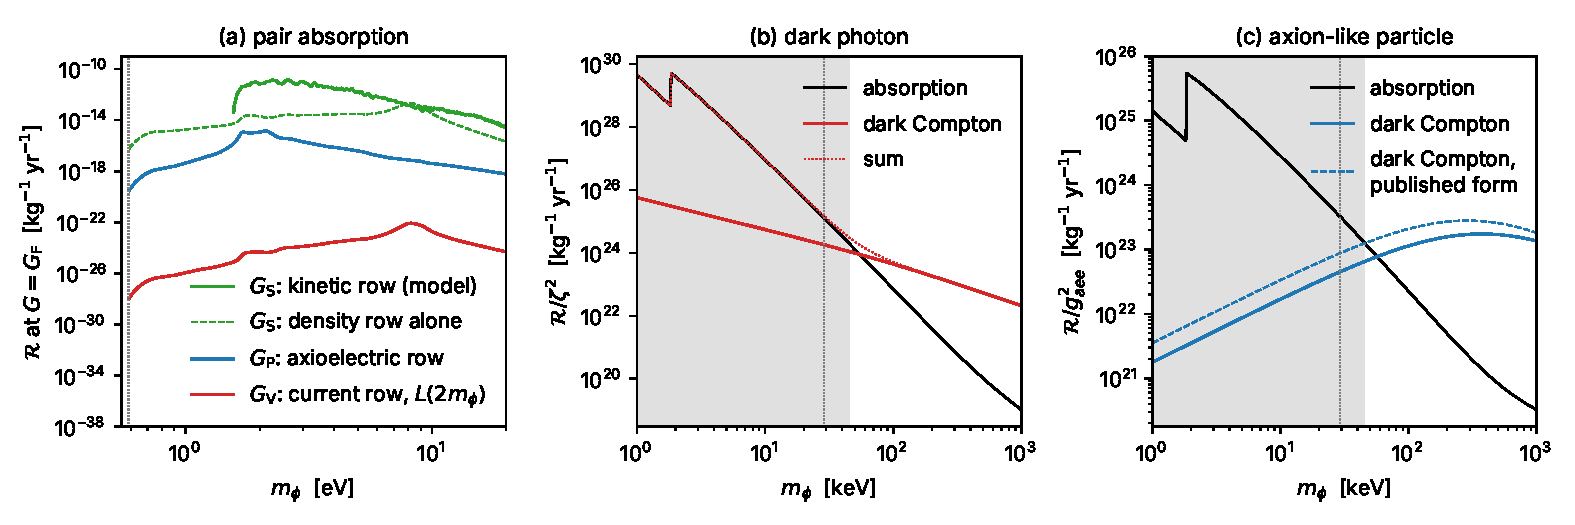
\includegraphics[width=\linewidth]{figures/ch10/fig10_7.pdf}
  \caption{Two-insertion rates of bosonic dark matter in silicon per kilogram-year, with $\rho_\chi = \SI{0.3}{GeV.cm^{-3}}$, $\rho_T = \SI{2.33}{g.cm^{-3}}$ and the halo of \cref{sec:1.2}. (a) Pair absorption of a complex scalar of mass $m_\phi$ at couplings $G = G_{\mathrm{F}}$, \cref{eq:10.8-contact}. Scalar through the kinetic row in the empirical-pseudopotential model of \cref{sec:10.7-scalar}, which has its own vertical gap at \SI{3.12}{eV} and is a model, not a prediction (solid green). Scalar through the density row alone with $\langle q^2\rangle^{1/2} = 2.14\times10^{-3}\,m_\phi$ and the measured loss function (dashed). Pseudoscalar, \cref{eq:10.8-P}, and vector, \cref{eq:10.8-V}, from the measured optical constants of float-zone silicon at \SI{300}{K}~\cite{franta2017temperature}, spliced at \SI{40}{eV} to atomic scattering factors~\cite{henke1993xray}. Dotted: $2m_\phi$ at the excitonic edge of cold silicon, \SI{1.1728}{eV} with $\Eg(0) = \SI{1.1692}{eV}$; the \SI{300}{K} data are wrong within tens of meV of it (\cref{sec:10.7-edge}). (b) Dark photon: absorption, \cref{eq:10.7-dp} (black; from the optical constants below \SI{29}{keV}, dotted line, and from the photoelectric cross section of the XCOM tables (the photon cross-section database of the National Institute of Standards and Technology)~\cite{berger2010xcom} above, with $\varepsilon = 1$), and dark Compton scattering on all 14 electrons, \cref{eq:10.8-compton} (red). (c) Axion-like particle: absorption, \cref{eq:10.7-alp} (black), and dark Compton scattering, \cref{eq:10.8-alpC} (blue). Gray in (b) and (c): $m_\phi < \SI{45}{keV}$, where the electron recoil $\omega_{\mathrm{C}}$ falls below the K-shell binding of \SI{1.84}{keV} and counting all 14 electrons as free overstates the Compton rate.}
  \label{fig:10-twoins}
\end{figure}

The reduction to \cref{eq:10.8-contact} assumes a smooth response. A target with a sharp line at $\Delta E$ resolves the kinetic energy of the pair instead: the rate is spread over $2m_\phi$ between $\Delta E - 4\bar K_{\mathrm{pair}}$ and $\Delta E$, and the peak it reaches depends on how the width of the line compares with $\bar K_{\mathrm{pair}}$. This is the regime of the atomic transitions of Ref.~\cite{bauer2026dark}, whose line shape follows the kinetic-energy distribution of the pair. In silicon the absorption continua vary on scales of meV, and \cref{eq:10.8-contact} holds; only a line narrower than $\bar K_{\mathrm{pair}}$, about \SI{1.6}{\micro eV} at $m_\phi = \SI{1}{eV}$, would resolve the kinetic energy of the pair. \Cref{lim:10.8a} shows where the reduction fails.

\begin{limitbox}[Pair absorption][lim:10.8a]
Pair absorption as single absorption at $\omega = 2m_\phi$ and $\vect{q} \to 0$, \cref{eq:10.8-contact}, with the constant coefficients $m_eG_{\mathrm{S}}$, $m_eG_{\mathrm{P}}$ and the velocity-dependent $G_{\mathrm{V,A}}(p - \bar p)^\mu$~\cite[Eqs.~(3) and (5)--(8)]{bauer2026dark}.
\par\smallskip
{\centering
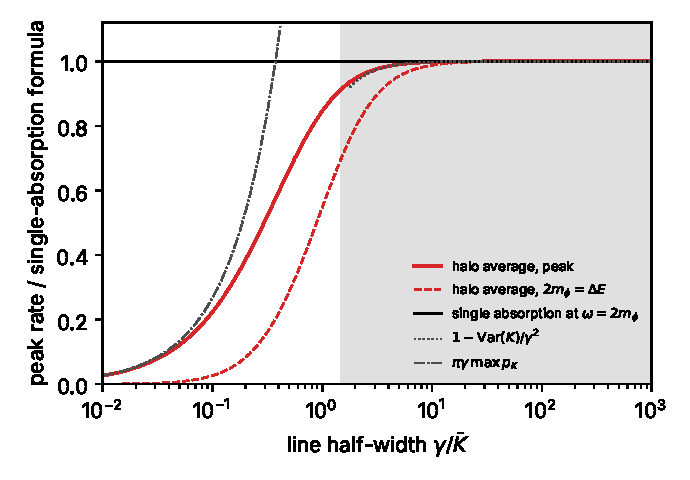
\includegraphics[width=0.72\linewidth]{figures/ch10/limit10_8a.pdf}
\captionof{figure}{Peak absorption rate of a model target with one Lorentzian line of half-width $\gamma$, as the halo average of \cref{eq:10.8-pair} over the pair kinetic energy $K_{\mathrm{pair}}$ (red), divided by the single-absorption formula \cref{eq:10.8-contact} (black), against $\gamma/\bar K_{\mathrm{pair}}$ with $\bar K_{\mathrm{pair}} = m_\phi\langle v^2\rangle = 1.60\times10^{-6}\,m_\phi$. Solid red: peak over the detuning $\Delta E - 2m_\phi$; dashed: at $2m_\phi = \Delta E$. Dotted: the leading correction for broad lines, $1 - \mathrm{Var}(K_{\mathrm{pair}})/\gamma^2$ with $\mathrm{Var}(K_{\mathrm{pair}}) = 0.253\,\bar K_{\mathrm{pair}}^2$; dash-dotted: the narrow-line limit $\pi\gamma\max p_K$, with $p_K$ the distribution of $K_{\mathrm{pair}}$, which the formula of Ref.~\cite{bauer2026dark} for a discrete transition reproduces. Halo of \cref{sec:1.2}, $2\times10^6$ velocity pairs; the dependence on $\vect{q}$ is dropped ($qa < 10^{-4}$). Gray: $\gamma \ge 1.5\,\bar K_{\mathrm{pair}}$, peak within \SI{10}{\percent} of the formula.}\label{fig:10-pair-limit}
\par}
\smallskip
For a line narrower than about $\bar K_{\mathrm{pair}}$, \SI{1.6}{\micro eV} at $m_\phi = \SI{1}{eV}$, the deposited energy follows the kinetic-energy distribution of the pair, and the formula overestimates the peak by $\bar K_{\mathrm{pair}}/\gamma$ up to a factor of order one.
\end{limitbox}

The pair-absorption rates need nothing that single absorption does not already compute: the absorption tables of the charge-like rows and the spin responses at $(\vect{q} \simeq 0, 2m_\phi)$, with the velocity moments of the vector and axial coefficients taken over two copies of the halo.

\subsection{Dark Compton scattering}\label{sec:10.8-compton}

A dark photon couples to the electrons as a photon does, with $e$ replaced by $\zeta e$ (\cref{sec:1.4}). An electron in the field of both therefore sees the total vector potential $\vect{A} + \zeta\vect{A}'$, and its Hamiltonian is $(\vect{p} + e\vect{A} + \zeta e\vect{A}')^2/2m_e$ plus the Pauli term. Expanded, it has the two linear couplings $(e/m_e)\vect{A}\cdot\vect{p}$ and $(\zeta e/m_e)\vect{A}'\cdot\vect{p}$, symmetrized, and a seagull that contains both fields at one point, $(\zeta e^2/m_e)\,\vect{A}\cdot\vect{A}'$. Absorbing a dark photon of polarization $\hat{\vect{e}}$ and emitting a photon of momentum $\vect{k}_\gamma$, energy $\omega_\gamma = |\vect{k}_\gamma|$ and polarization $\hat{\vect{e}}_\gamma$ is a process with two insertions. The seagull does it at first order, and the linear couplings at second order through \cref{eq:10.8-T2}. Per unit amplitude of each field, the target sees the transition operator
\begin{equation}
  T^{\mathrm{C}} = \frac{\zeta e^2}{m_e}\,(\hat{\vect{e}}\cdot\hat{\vect{e}}_\gamma^*)\,n_e(\vect{q})
  + \zeta e^2\Bigl[\hat{\vect{e}}_\gamma^*\cdot\vect{j}_e\,\frac{1}{E_i + m_\phi - H_0}\,\hat{\vect{e}}\cdot\vect{j}_e
  + \hat{\vect{e}}\cdot\vect{j}_e\,\frac{1}{E_i - \omega_\gamma - H_0}\,\hat{\vect{e}}_\gamma^*\cdot\vect{j}_e\Bigr] ,
  \label{eq:10.8-TC}
\end{equation}
with the momentum transfer $\vect{q} = \vect{p}_\phi - \vect{k}_\gamma \simeq -\vect{k}_\gamma$ and the current rows $\vect{j}_e$ at the momenta of their own fields. Both fields carry the factor $1/\sqrt{2\omega \Vol}$ of a quantum of energy $\omega$, as in \cref{eq:8.2-abs}. Summed over the momenta and polarizations of the photon, the golden rule gives the rate per dark photon
\begin{equation}
  \varGamma = \int\frac{\dd^3k_\gamma}{(2\pi)^3\,2\omega_\gamma}\,\frac{1}{2m_\phi}\sum_{\hat{\vect{e}}_\gamma}S_{T^{\mathrm{C}}T^{\mathrm{C}}}(\vect{q},\, m_\phi - \omega_\gamma) ,
  \label{eq:10.8-CS}
\end{equation}
averaged over the three polarizations $\hat{\vect{e}}$ of the dark photon. The target takes the energy $\omega = m_\phi - \omega_\gamma$ and the momentum $\vect{q}$, whose size is close to $m_\phi$. A dark photon of \SI{100}{keV} probes the electrons at $|\vect{q}| = \SI{92}{keV}$, or \SI{47}{\angstrom^{-1}}, far beyond every reciprocal-lattice vector and every inverse orbital radius except those of the innermost shells.

\emph{The Thomson limit.} For a free electron at rest both second-order terms vanish. If the dark photon is absorbed first, its vertex $\hat{\vect{e}}\cdot\vect{p}$ acts on an electron at rest, with $\vect{p}_\phi$ negligible. If the photon is emitted first, its vertex is $\hat{\vect{e}}_\gamma^*\cdot(\vect{p}_i + \vect{p}_m)/2 = -\hat{\vect{e}}_\gamma^*\cdot\vect{k}_\gamma/2 = 0$, since the photon is transverse. Only the seagull remains, and $S_{nn}(\vect{q},\omega) = 2\pi\nd_e\,\delta(\omega - q^2/2m_e)$ for electrons at rest. For $m_\phi \ll m_e$ each electron then scatters the dark photon with the cross section $\zeta^2\sigma_{\mathrm{Th}}$, with $\sigma_{\mathrm{Th}} = e^4/6\pi m_e^2 = \SI{6.65e-25}{cm^2}$ the Thomson cross section, isotropically, since the massive vector has three polarizations, and the electron keeps the recoil energy $m_\phi^2/2m_e$.

In a crystal the seagull row is the density at $|\vect{q}| \simeq m_\phi$, and \cref{eq:10.8-CS} needs $S_{nn}$ at large momentum. There the dark matter resolves single electrons, and the impulse approximation of \cref{we:4-gas} applies, as for the core shells of \cref{sec:10.6}. An electron whose binding is small against the recoil scatters as if free, and its deposit is a line at the free recoil, broadened by its momentum in the atom: the Compton profile of its shell. The binding corrections are the second-order terms of \cref{eq:10.8-TC}, which no longer vanish for a bound electron. An electron bound more strongly than the recoil can absorb barely contributes. In silicon the recoil reaches the K-shell binding, \SI{1.84}{keV}, at $m_\phi = \SI{45}{keV}$, and the L-shell binding, about \SI{100}{eV}, at \SI{10}{keV}. Above \SI{45}{keV} all 14 electrons count, $\nd_e/\rho_T = 3.00\times10^{23}\,\mathrm{g}^{-1}$. The medium also changes the phase space of the photon through the refractive index $n_r(\omega_\gamma) = 1 - \omega_p^2/2\omega_\gamma^2$. It differs from one by $2\times10^{-7}$ at \SI{50}{keV} with the all-electron $\omega_p = \SI{31.1}{eV}$. The in-medium mixing of the dark photon is, at these masses, the vacuum mixing (\cref{sec:10.7-darkphoton}).

\emph{The exact tree-level rate.} The relativistic amplitude of $V + e \to \gamma + e$ consists of the two Compton diagrams with one photon made massive. Squared, summed over the spins of the electrons and the polarizations of the photon, and averaged over the three polarizations of the dark photon, it is a standard Dirac trace. The term $k^\mu k^\nu/m_\phi^2$ of the massive polarization sum drops out because the electron current is conserved, $k_\mu\mathcal{M}^\mu = 0$. Hochberg, von Krosigk, Kuflik and Yu evaluated the trace and integrated it over the final states~\cite[Eqs.~(7)--(12)]{hochberg2022impact}. For a dark photon and an electron at rest the photon energy is fixed by two-body kinematics at $\omega_\gamma = m_\phi(m_\phi + 2m_e)/2(m_\phi + m_e)$, the electron takes
\begin{equation*}
  \omega_{\mathrm{C}} = m_\phi - \omega_\gamma = \frac{m_\phi^2}{2(m_\phi + m_e)} ,
\end{equation*}
and the rate per dark photon is~\cite[Eq.~(2)]{hochberg2022impact}
\begin{equation}
  \varGamma = \nd_e\,\zeta^2\,\frac{e^4}{24\pi m_e^2}\,\frac{(m_\phi + 2m_e)(m_\phi^2 + 2m_em_\phi + 2m_e^2)}{(m_\phi + m_e)^3} ,
  \label{eq:10.8-compton}
\end{equation}
with their kinetic mixing $\varepsilon$ written as $\zeta$. The event rate per unit mass is $(\rho_\chi/m_\phi\rho_T)\varGamma$. At threshold the traces give the averaged squared amplitude $|\bar{\mathcal{M}}|^2 = \frac43e^4\zeta^2(m_\phi^2 + 2m_em_\phi + 2m_e^2)/[m_e(m_\phi + m_e)]$, and with the two-body phase space, $\varGamma = \nd_e|\bar{\mathcal{M}}|^2\omega_\gamma/[16\pi m_\phi m_e(m_\phi + m_e)]$, this is \cref{eq:10.8-compton} exactly, at every $m_\phi/m_e$. It is the exact tree-level rate on a free electron at rest; it tends to the Thomson rate $\nd_e\zeta^2\sigma_{\mathrm{Th}}$ for $m_\phi \ll m_e$ and to a quarter of it for $m_\phi \gg m_e$.

\Cref{fig:10-twoins}b compares dark Compton scattering in silicon with absorption. Absorption falls with the photoelectric cross section, roughly as $m_\phi^{-3}$ per particle above the K edge, while the Compton rate per particle hardly changes below $m_e$. The two cross at $m_\phi = \SI{55}{keV}$, and at \SI{100}{keV} dark Compton scattering is 6.2 times more frequent. In germanium, whose photoelectric cross section is 15 times larger at \SI{100}{keV}, they cross at \SI{144}{keV}. The photon that leaves carries most of the energy, \SI{92}{keV} at $m_\phi = \SI{100}{keV}$, and travels about \SI{2}{cm} in silicon before it interacts~\cite{berger2010xcom}.

\emph{Axion-like particles.} An axion-like particle couples to the spin current of the electrons through $(\partial_t\phi)$, the second term of \cref{eq:1.4-alp}. Minimal coupling turns the gradient in that term into $\nabla + \ii e\vect{A}$ for an electron of charge $-e$, and the spin current $\psi^\dagger\boldsymbol{\sigma}\cdot\overleftrightarrow{\nabla}\psi$ acquires $2\ii e\vect{A}\cdot\psi^\dagger\boldsymbol{\sigma}\psi$. Multiplied by $\ii g_{aee}(\partial_t\phi)/4m_e^2$ this is a seagull for the axion-like particle,
\begin{equation*}
  H_{\mathrm{sg}} = \frac{e\,g_{aee}}{m_e^2}\,(\partial_t\phi)\,\vect{A}\cdot\vect{s}_e ,
\end{equation*}
which absorbs the particle and emits a photon at one point by flipping, or not flipping, a spin. For a free electron at rest the second-order terms of the photon's orbital coupling vanish as for the dark photon, but the Pauli coupling of the photon to the spin, joined to the spin current of the particle, adds second-order terms at relative order $x = m_\phi/m_e$. The exact tree-level rate, from the Lagrangian $g_{aee}\phi\,\bar\psi\ii\gamma^5\psi$ and the same two diagrams with the pseudoscalar vertex $\gamma^5$ (here the photon polarization sum is the only one), is
\begin{equation}
  \varGamma = \nd_e\,\frac{e^2g_{aee}^2}{16\pi m_e^2}\,\frac{m_\phi^2\,(m_\phi + 2m_e)}{(m_\phi + m_e)^3} ,
  \label{eq:10.8-alpC}
\end{equation}
whose expansion in $x$ starts as $\nd_e(e^2g_{aee}^2m_\phi^2/8\pi m_e^4)(1 - \frac52x + \frac92x^2)$, the spin seagull at leading order. The squared amplitude behind it agrees, at every mass, with the one printed in Ref.~\cite[Eq.~(15)]{hochberg2022impact}. \Cref{fig:10-twoins}c shows the rate in silicon: dark Compton scattering overtakes absorption of an axion-like particle at \SI{57}{keV}.

\begin{workedexample}{The axion-like Compton rate at \SI{100}{keV}}\label{we:10-alpcompton}
At $m_\phi = \SI{100}{keV}$, $x = 0.1957$. The photon leaves with $\omega_\gamma = m_\phi(m_\phi + 2m_e)/2(m_\phi + m_e) = \SI{91.82}{keV}$, and the electron takes $\omega_{\mathrm{C}} = \SI{8.18}{keV}$, above the K-shell binding of silicon and below that of germanium, \SI{11.1}{keV}. Per electron and per unit coupling, \cref{eq:10.8-alpC} gives $\varGamma/(\nd_eg_{aee}^2) = \SI{1.34e-25}{cm^2}$ times the speed of light.

In silicon, with $\nd_e/\rho_T = 3.00\times10^{23}\,\mathrm{g}^{-1}$ and the photoelectric cross section $\SI{0.0250}{cm^2/g}$ at \SI{100}{keV}, the Compton rate of \cref{eq:10.8-alpC} is 5.1 times the absorption rate of \cref{eq:10.7-alp}. In germanium absorption still dominates at this mass: the Compton rate is 0.30 of it.
\end{workedexample}

\subsection{Open problems}\label{sec:10.8-open}

Two pieces of the two-insertion response are not computed for any crystal. The first is the interference between a contact amplitude and a second-order one, which a dark-matter model with both kinds of coupling produces. For the stopping of a charged particle the same term is the Barkas correction, odd in the charge of the projectile. It is linear in the quadratic response of the target, a three-point function, and no reduction to two-point responses exists. The quadratic response of the electron gas is known and serves as a check. The second is the bound-state correction to dark Compton scattering for the shells whose binding is close to $\omega_{\mathrm{C}}$. They are the K shell of silicon between 45 and about \SI{100}{keV}, the K shell of germanium, whose binding of \SI{11.1}{keV} the recoil reaches at \SI{118}{keV}, and the L shells below about \SI{20}{keV}. There the second-order terms of \cref{eq:10.8-TC} no longer vanish, and the rate needs the shell Compton profiles or the large-$q$ density response, together with the refractive index at the photon energy.

\section{Inelastic and relativistic dark matter}\label{sec:10.9}

A dark-matter particle of \SI{1}{MeV} that arrives in an excited state \SI{10}{eV} above its ground state carries three times more energy in its mass splitting than in its motion, whose kinetic energy is at most \SI{3.5}{eV}. A particle accelerated by a cosmic-ray electron can move at nearly the speed of light, and a fermion that is absorbed hands over almost its whole rest energy. Each of these cases changes one ingredient of the master formula of \cref{sec:8.2} and leaves the others alone. A mass splitting changes the kinematics, through the term $-\Delta_\chi$ in $\omega_{\vect{q}}$. A relativistic particle changes the dark-matter tensor $\mathfrak{D}_{ab}$, and an outgoing light fermion changes both. The target enters, as before, through the response matrix of the rows of \cref{eq:8.1-rows}, and the silicon tables of \cref{sec:10.2} provide it.

\subsection{Inelastic and exothermic scattering}\label{sec:10.9-inelastic}

For inelastic dark matter the potential and $\sigmae$ keep their elastic form (\cref{sec:1.4}). The time component of the current that connects $\chi_1$ to $\chi_2$ reduces to one, as for the elastic current, up to corrections of order $\Delta_\chi/\mchi$ (\cref{eq:C.15-bilinears}), and the recoil term of \cref{eq:8.1-omega-inel} is smaller by the same fraction. The only change that matters is the term $-\Delta_\chi$ in $\omega_{\vect{q}}$. The derivation of \cref{sec:10.2} then goes through step by step. The angular integral of \cref{eq:A.8-eta} produces $\eta$ at the minimum velocity of \cref{eq:1.3-vmin}, taken in absolute value:
\begin{keyresult}[Inelastic electron-recoil rate]
\begin{equation}
  \frac{\dd\mathcal{R}}{\dd\omega} = \frac{\rho_\chi\,\sigmae}{8\pi^2\alpha\,\rho_T\,\mchi\,\mu_{\chi e}^2}\int\dd q\;q^3\,\eta\bigl(\vmin\bigr)\,\FDM(q)^2\,\bar L(q,\omega) , \qquad
  \vmin = \left|\frac{\omega + \Delta_\chi}{q} + \frac{q}{2\mchi}\right| ,
  \label{eq:10.9-inel}
\end{equation}
at $T = 0$, with $\bar L$ the loss function averaged over the directions of $\vect{q}$. It is exact under the conditions of \cref{eq:10.2-rate}.
\end{keyresult}
\noindent The absolute value is needed only when $\omega + \Delta_\chi < 0$, which at $T = 0$ means exothermic dark matter depositing less than $|\Delta_\chi|$.

An endothermic splitting is paid from the kinetic energy. Since $\omega \le \tfrac12\mchi v^2 - \Delta_\chi$ (\cref{eq:1.3-omegamax}), a pair across the gap needs $\mchi \ge 2(\Delta_\chi + \Eg)/v_{\mathrm{max}}^2$: \SI{0.60}{MeV} for $\Delta_\chi = \SI{1}{eV}$ and \SI{3.2}{MeV} for \SI{10}{eV}, with the step-model gap of \SI{1.11}{eV} that accompanies the tables of \cref{sec:10.2}. An exothermic splitting is paid by the dark matter, and as \cref{sec:8.2-exothermic} found, it shifts the band of allowed $(q,\omega)$ up by $|\Delta_\chi|$, down to $q \to 0$. \Cref{fig:10-inelastic} shows the consequence in silicon at \SI{10}{MeV}. With a heavy mediator, per kilogram-year at $\sigmae = \SI{e-37}{cm^2}$, the rate is 314 events for $\Delta_\chi = \SI{10}{eV}$, $5.9\times10^4$ for elastic scattering and $7.5\times10^5$ for $\Delta_\chi = \SI{-10}{eV}$. With a light mediator the three numbers are 6.2, $9.8\times10^3$ and $5.2\times10^5$, and the exothermic spectrum has a sharp peak at $\omega = |\Delta_\chi|$. Splittings of a few eV move the rate by orders of magnitude, in either direction.

\begin{figure}[tbp]
  \centering
  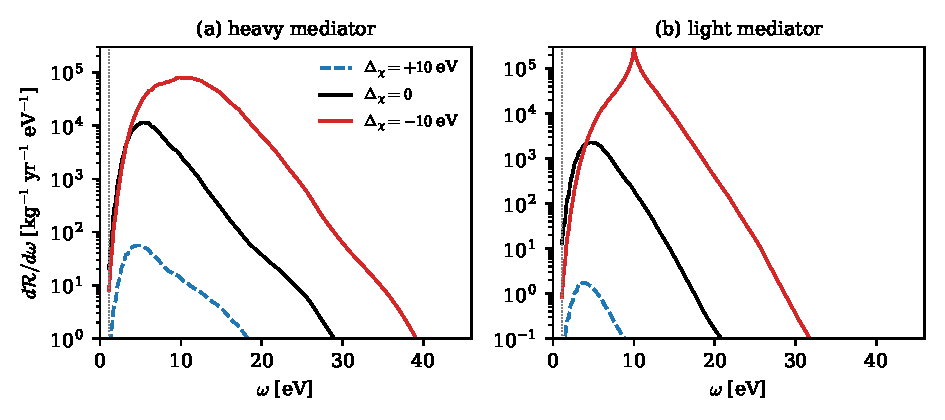
\includegraphics[width=\linewidth]{figures/ch10/fig10_8.pdf}
  \caption{Electron-recoil spectrum of silicon for inelastic dark matter of mass $\mchi = \SI{10}{MeV}$ with splittings $\Delta_\chi = \SI{+10}{eV}$ (endothermic, dashed), 0 (elastic) and \SI{-10}{eV} (exothermic), from \cref{eq:10.9-inel}. Inputs: the random-phase loss function with local fields of the tables of \cref{sec:10.2}, the standard halo of \cref{sec:1.2}, $\rho_\chi = \SI{0.3}{GeV.cm^{-3}}$ and $\sigmae = \SI{e-37}{cm^2}$. Dotted: \SI{1.11}{eV}, the step-model gap that accompanies the tables, below the low-temperature gap of \SI{1.17}{eV} to which their scissor shifts the bands. Below $|\vect{q}| = \SI{493}{eV}$, the first tabulated momentum, the loss function is held at its value there. (a) Heavy mediator, $\FDM = 1$. (b) Light mediator, $\FDM = (q_0/q)^2$; the exothermic spectrum peaks at $\omega = |\Delta_\chi|$, where the momentum transfer goes to zero.}
  \label{fig:10-inelastic}
\end{figure}

An exothermic particle is not limited by the kinetic energy of the halo, and its spectrum is set by the splitting. To see how, complete the square in $\omega_{\vect{q}}$ with $\Delta_\chi < 0$,
\begin{equation*}
  \omega_{\vect{q}} = |\Delta_\chi| + \vect{q}\cdot\vect{v} - \frac{q^2}{2\mchi} = |\Delta_\chi| + \tfrac12\mchi v^2 - \frac{|\vect{q} - \mchi\vect{v}|^2}{2\mchi} .
\end{equation*}
At fixed $\omega < |\Delta_\chi|$ the delta function of \cref{eq:8.2-spectrum} puts $\vect{q}$ on a sphere of radius $k_*$ centered at $\mchi\vect{v}$, with $k_*^2 = q_\Delta^2 + \mchi^2v^2$ and
\begin{equation*}
  q_\Delta = \sqrt{2\mchi\bigl(|\Delta_\chi| - \omega\bigr)} , \qquad v_\Delta = q_\Delta/\mchi .
\end{equation*}
For any function $G$ of $|\vect{q}|$, $\int\dd^3q\,\delta(\omega - \omega_{\vect{q}})\,G = \mchi k_*\int\dd^2\hat{\vect{n}}\,G(|\mchi\vect{v} + k_*\hat{\vect{n}}|)$. On the sphere $q^2 = k_*^2 + \mchi^2v^2 + 2k_*\mchi\vect{v}\cdot\hat{\vect{n}}$, and the term linear in $\vect{v}$ averages to zero because the sphere is centered at $\mchi\vect{v}$. The integral is therefore $4\pi\mchi q_\Delta G(q_\Delta)[1 + O(v^2/v_\Delta^2)]$, exactly $4\pi\mchi k_*G$ for constant $G$. The rate per particle no longer depends on its velocity, and the average over the halo is trivial. With $G = |\tilde V|^2\bar S$, $\bar S = (2q^2/e^2)\bar L$ and $\rho_\chi/\mchi\rho_T$ per unit mass,
\begin{keyresult}[Exothermic shell]
\begin{equation}
  \frac{\dd\mathcal{R}}{\dd\omega} = \frac{\rho_\chi\,\sigmae\,q_\Delta^3\,\FDM(q_\Delta)^2\,\bar L(q_\Delta,\omega)}{4\pi^2\alpha\,\rho_T\,\mu_{\chi e}^2}\,\Bigl[1 + O\bigl(v^2/v_\Delta^2\bigr)\Bigr] , \qquad \omega < |\Delta_\chi| ,
  \label{eq:10.9-shell}
\end{equation}
independent of the velocity distribution as long as $v_\Delta$ exceeds the speeds of the halo. The spectrum samples the response along the parabola $\omega = |\Delta_\chi| - q^2/2\mchi$.
\end{keyresult}
\noindent For constant $\bar L$ and a heavy mediator the correction is about $2.5\langle v^2\rangle/v_\Delta^2$, with $\langle v^2\rangle^{1/2} = 1.3\times10^{-3}$ in the laboratory frame: at $\mchi = \SI{0.1}{MeV}$ and $\omega = \SI{3}{eV}$, \cref{eq:10.9-inel} exceeds \cref{eq:10.9-shell} by \SI{2.9}{\percent}. Since $v_\Delta^2 = 2(|\Delta_\chi| - \omega)/\mchi$, the shell form needs $\mchi$ well below $2|\Delta_\chi|/v_{\mathrm{max}}^2$, which is \SI{2.9}{MeV} for $|\Delta_\chi| = \SI{10}{eV}$; at \SI{10}{MeV} the halo still matters, and \cref{fig:10-inelastic} uses \cref{eq:10.9-inel}.

The parabola explains where exothermic spectra peak. On a free electron at rest the response is a line, $S \propto \delta(\omega - q^2/2m_e)$, and it crosses the parabola once, at
\begin{equation*}
  \omega_{\mathrm{line}} = \frac{\mu_{\chi e}}{m_e}\,|\Delta_\chi| , \qquad q_{\mathrm{line}} = \sqrt{2\mu_{\chi e}|\Delta_\chi|} ,
\end{equation*}
the energy shared between the two recoiling particles. A heavy dark-matter particle hands the whole splitting to the electron, and a light one keeps part of it. In a crystal the electron line exists only where the free-electron picture holds, $q_{\mathrm{line}} \gg q_0$, that is $\omega_{\mathrm{line}} \gg q_0^2/2m_e = \SI{13.6}{eV}$. For smaller splittings the parabola crosses the region in which the response is that of bound electrons, and the peak sits where $q_\Delta^3\bar L$ is largest. The factor $q_\Delta^3$ falls toward $\omega = |\Delta_\chi|$, while $\bar L$ rises from the gap toward the plasma frequency, and the product peaks in between.

A light mediator turns the end of the spectrum into a line. As $\omega \to |\Delta_\chi|$, $q_\Delta \to 0$ and $\bar S \to (q^2/2\pi\alpha)L(0,\omega)$, the optical limit, so that with $\FDM^2 = q_0^4/q^4$
\begin{equation}
  \frac{\dd\mathcal{R}}{\dd\omega} \to \frac{\rho_\chi\,\sigmae\,q_0^4\,L(0,\omega)}{4\pi^2\alpha\,\rho_T\,\mu_{\chi e}^2\,q_\Delta} \propto \bigl(|\Delta_\chi| - \omega\bigr)^{-1/2} .
  \label{eq:10.9-edge}
\end{equation}
The divergence is integrable. Within $\tfrac12\mchi v^2$ of the end point, where $v_\Delta$ falls below the halo speeds, the exact kernel softens it to a logarithm, since there the momentum transfer can go to zero for every speed of the halo. Its strength is the optical loss function at $\omega = |\Delta_\chi|$: near the end point the exothermic particle acts like a boson of mass $|\Delta_\chi|$ absorbed at $\vect{q} \simeq 0$ (\cref{sec:8.2-exothermic}), and like the dark photon of \cref{sec:10.7} it reads $L$ rather than $\varepsilon_2$.

\begin{workedexample}{Exothermic lines in silicon}\label{we:10-exo}
Take $\Delta_\chi = \SI{-10}{eV}$ in silicon and the masses 0.1, 0.3, 1 and \SI{3}{MeV}. The free-electron lines would sit at $\omega_{\mathrm{line}} = 1.64$, 3.70, 6.62 and \SI{8.54}{eV}, at $q_{\mathrm{line}} = 1.29$, 1.94, 2.60 and \SI{2.96}{keV}. Every one of these momenta lies below $q_0 = \SI{3.73}{keV}$; even an infinitely heavy particle reaches only $q_{\mathrm{line}} = (2m_e|\Delta_\chi|)^{1/2} = \SI{3.20}{keV}$. A \SI{10}{eV} splitting therefore never meets free electrons in silicon.

The silicon spectrum from \cref{eq:10.9-inel}, with the random-phase loss function with local fields and a heavy mediator, peaks at 6.95, 6.19, 5.99 and \SI{7.29}{eV} for the four masses, with half-maximum edges between about 4 and \SI{8.5}{eV} (up to \SI{11.8}{eV} at \SI{3}{MeV}). At \SI{0.1}{MeV} the peak lies \SI{5.3}{eV} above the free-electron line, at \SI{1}{MeV} \SI{0.6}{eV} below it: the peak barely moves with the mass because it is set by the loss function, not by the recoil. The momentum transfer at the peak is $q_\Delta = 0.78$, 1.51, 2.83 and \SI{4.03}{keV}, from $0.21\,q_0$ to $1.08\,q_0$. Per kilogram-year at $\sigmae = \SI{e-37}{cm^2}$ the totals are $2.1\times10^5$, $3.1\times10^5$, $8.7\times10^5$ and $1.5\times10^6$. The shell form \cref{eq:10.9-shell} reproduces them to 0.91, 0.81, 0.63 and 0.73. The largest speeds of the halo reach $v_\Delta$ at the peak for $\mchi \gtrsim \SI{1}{MeV}$, with $v_{\mathrm{max}}/v_\Delta = 0.34$, 0.53, 0.94 and 1.97. At the lightest mass the residual comes from the tables: binned in \SI{100}{eV} steps of $|\vect{q}|$, the loss function varies by about \SI{15}{\percent} from bin to bin at these momenta, and the shell form samples a single $q$.

With a light mediator every mass gives a line at $\omega = \SI{10.0}{eV}$, an integrable cusp whose width is set by the energy resolution of the detector rather than by the halo. The last \SI{0.5}{eV} below $|\Delta_\chi|$ holds 40, 42, 47 and \SI{60}{\percent} of the rate, and the \SI{0.1}{eV} around $|\Delta_\chi|$ holds 15, 12, 8 and \SI{6.5}{\percent}. Its height follows from \cref{eq:10.9-edge} with $L(0,\SI{10}{eV})$, which is 0.247 measured (\cref{we:10-darkphoton}) and 0.218 in the first bin of the tables. The two mediators therefore leave different signatures for the same splitting: a broad bump near \SI{6}{eV} whose position hardly depends on the mass, or a line at the splitting itself. Neither sits at $\mu_{\chi e}|\Delta_\chi|/m_e$.
\end{workedexample}

Nothing new is needed from the material: \cref{eq:10.9-inel} uses the same loss functions as the elastic rate, now on a grid of $\omega$ that extends to $|\Delta_\chi| + \tfrac12\mchi v_{\mathrm{max}}^2$, and the light-mediator line needs the optical limit, which measurements give. Above \SI{99}{eV} the $2p$ shell of silicon opens (\cref{sec:10.6}), and the valence tables no longer suffice.

\subsection{Boosted dark matter}\label{sec:10.9-boosted}

A light halo particle can be accelerated after it leaves the halo's equilibrium. Cosmic-ray electrons and protons of MeV to GeV energies cross the dark-matter halo of the Galaxy, and a small fraction of them scatter on dark-matter particles along the way, which then carry kinetic energies comparable to their mass. The resulting flux at the Earth is the line-of-sight integral of the dark-matter density times the cosmic-ray flux and the scattering cross-section. For electrons, Liang and collaborators write it as $\dd\Phi_\chi/\dd T_\chi = D_{\mathrm{eff}}(\rho_\chi/\mchi)\int\dd T_e\,(\dd\sigma_{\chi e}/\dd T_\chi)(\dd\Phi_e/\dd T_e)$, with $T_\chi$ and $T_e$ the kinetic energies and $D_{\mathrm{eff}} = \SI{8.02}{kpc}$ an effective distance for a halo profile integrated to \SI{10}{kpc}~\cite[Eq.~(1)]{liang2025plasmon}. The flux is small, since only one halo particle in many meets a cosmic ray, but it reaches speeds close to that of light and with them energies far above $\tfrac12\mchi v_{\mathrm{max}}^2$.

The Sun accelerates a second component. Halo particles that fall into it scatter on the electrons of the solar core, at $1.57\times10^7$\,K at the center~\cite[Table~5]{bahcall2001solar}, whose thermal speed $(3T/m_e)^{1/2}$ is about 0.09. Some leave with speeds of that order, far above the escape speed of the Galaxy but well below that of light. The DAMIC-M collaboration, Dark Matter in CCDs (DAMIC) at Modane, has searched for this solar-reflected component~\cite{aggarwal2026constraints}. In both cases the halo average of \cref{eq:8.2-spectrum} is replaced by an average over the flux. For a flux that is isotropic in the laboratory, the number density per unit speed is $(\dd\Phi_\chi/\dd v)/v$, and the non-relativistic rate keeps its form with
\begin{equation*}
  \frac{\rho_\chi}{\mchi}\,\eta(\vmin) \;\to\; \int_{\vmin}\dd v\;\frac{1}{v^2}\,\frac{\dd\Phi_\chi}{\dd v} ,
\end{equation*}
the replacement of Ref.~\cite[Eqs.~(9)--(11)]{aggarwal2026constraints}. The real fluxes are anisotropic, the solar one pointing away from the Sun, and the angular average of the response that makes $\eta$ sufficient is then an assumption. For speeds near that of light the non-relativistic rows themselves must be checked.

The non-relativistic potential of \cref{sec:8.1} assumed that the energy deposited is small against the momentum transfer, so that the mediator acts instantaneously. For a relativistic particle $\omega$ can approach $q$, and the mediator must be kept whole. Take a vector mediator of mass $m_V$ coupled with strengths $y_\chi$ and $y_e$ to the dark-matter current $J^\mu_\chi = \bar u(p')\gamma^\mu u(p)$ and to the electron current $J^\mu_e = (n_e, \vect{j}_e)$. We write $\mathcal{Q} = |\vect{q}|$ for the momentum transfer, to keep it apart from the four-momentum, and $E_\chi = (p^2 + \mchi^2)^{1/2}$ for the energy, so that $\omega = E_\chi(\vect{p}) - E_\chi(\vect{p} - \vect{q})$ by \cref{eq:8.1-omega}. The amplitude is $y_\chi y_e(J^0_\chi n_e - \vect{J}_\chi\cdot\vect{j}_e)/(\mathcal{Q}^2 - \omega^2 + m_V^2)$. Both currents are conserved. For the target, \cref{eq:4.3-continuity} gives $\hat{\vect{q}}\cdot\vect{j}_e \to (\omega/\mathcal{Q})n_e$ between eigenstates; for the dark matter, the Dirac equation gives $\hat{\vect{q}}\cdot\vect{J}_\chi = (\omega/\mathcal{Q})J^0_\chi$. Splitting each spatial current into its part along $\hat{\vect{q}}$ and its transverse part, $\vect{J}_\chi\cdot\vect{j}_e = (\omega^2/\mathcal{Q}^2)J^0_\chi n_e + \vect{J}_{\chi\mathrm{T}}\cdot\vect{j}_{e\mathrm{T}}$, and the amplitude becomes
\begin{equation}
  y_\chi y_e\,\frac{J^0_\chi\,n_e\,(1 - \omega^2/\mathcal{Q}^2) - \vect{J}_{\chi\mathrm{T}}\cdot\vect{j}_{e\mathrm{T}}}{\mathcal{Q}^2 - \omega^2 + m_V^2} .
  \label{eq:10.9-amp}
\end{equation}
For a massless mediator the density term is $J^0_\chi n_e/\mathcal{Q}^2$, the instantaneous Coulomb interaction, and only the transverse term propagates at the speed of light. Retardation enters the density row of a massive mediator as the factor $(1 - \omega^2/\mathcal{Q}^2)$, and it comes from keeping the longitudinal current, which continuity ties to the density.

The density row needs the spin average of $|J^0_\chi|^2$. Write $\gamma\cdot p = \gamma^\mu p_\mu$ for the four-momentum $p = (E_\chi, \vect{p})$. The spinors of \cref{eq:C.15-spinor} obey $\sum_su(p,s)\bar u(p,s) = \gamma\cdot p + \mchi$, and the traces needed are $\Tr(\gamma^\mu\gamma^\nu) = 4g^{\mu\nu}$, $\Tr(\gamma^\mu\gamma^\nu\gamma^\rho\gamma^\sigma) = 4(g^{\mu\nu}g^{\rho\sigma} - g^{\mu\rho}g^{\nu\sigma} + g^{\mu\sigma}g^{\nu\rho})$, and zero for an odd number of matrices. Then
\begin{equation*}
  \begin{aligned}
  \frac12\sum_{s,s'}\bigl|\bar u(p',s')\gamma^0u(p,s)\bigr|^2 &= \frac12\Tr\bigl[(\gamma\cdot p' + \mchi)\gamma^0(\gamma\cdot p + \mchi)\gamma^0\bigr] \\
  &= 2\bigl(E_\chi E'_\chi + \vect{p}\cdot\vect{p}' + \mchi^2\bigr) = (2E_\chi - \omega)^2 - \mathcal{Q}^2 ,
  \end{aligned}
\end{equation*}
where the four-matrix trace gives $4(2E'_\chi E_\chi - p'\cdot p)$ with $p'\cdot p = E'_\chi E_\chi - \vect{p}'\cdot\vect{p}$, and the last step uses $E'_\chi = E_\chi - \omega$ and $2\vect{p}\cdot\vect{p}' = p^2 + p'^2 - \mathcal{Q}^2$. Dividing by the normalization $2E_\chi\cdot2E'_\chi$ of the two dark-matter states, squaring \cref{eq:10.9-amp} and writing the couplings through $\sigmae$ as in \cref{eq:1.4-Vsq},
\begin{keyresult}[Relativistic density row]
\begin{equation}
  \mathfrak{D}_{nn} = \frac{\pi\sigmae}{\mu_{\chi e}^2}\;\frac{(2E_\chi - \omega)^2 - \mathcal{Q}^2}{4E_\chi(E_\chi - \omega)}\;\Bigl(1 - \frac{\omega^2}{\mathcal{Q}^2}\Bigr)^2\left[\frac{q_0^2 + m_V^2}{\mathcal{Q}^2 - \omega^2 + m_V^2}\right]^2 ,
  \label{eq:10.9-Drel}
\end{equation}
which tends to $\pi\sigmae\FDM^2/\mu_{\chi e}^2$ as $v \to 0$. The rate per particle is \cref{eq:8.2-rate} with $S_{nn} = (2\mathcal{Q}^2/e^2)\bar L$, and per unit target mass $\dd\mathcal{R}/\dd\omega = \rho_T^{-1}\int\dd v\,v^{-1}(\dd\Phi_\chi/\dd v)\,\dd\varGamma/\dd\omega$ for an isotropic flux.
\end{keyresult}
\noindent This constructs the relativistic tensor that \cref{sec:8.2-absorption} left open, for the density row. The transverse row enters through $\vect{J}_{\chi\mathrm{T}}$, whose square for a particle much heavier than the energy deposited is $4E_\chi^2v_{\mathrm{T}}^2$, with $v_{\mathrm{T}}^2 = v^2 - (\vect{v}\cdot\hat{\vect{q}})^2 = v^2 - \omega^2/\mathcal{Q}^2$. For a massless mediator the medium answers a transverse current through its transverse dielectric function $\varepsilon^{\mathrm{T}}$ of \cref{sec:4.4}, and the propagator $1/\mathcal{Q}^2$ of the density row becomes $1/(\mathcal{Q}^2 - \omega^2\varepsilon^{\mathrm{T}})$ in the transverse row. After averaging over the directions of $\vect{q}$ the density and the transverse current are uncorrelated, and the two rows add. The loss function of the density row is replaced by
\begin{equation}
  \bar L(\mathcal{Q},\omega) \;\to\; \bar L(\mathcal{Q},\omega) + \Bigl(v^2 - \frac{\omega^2}{\mathcal{Q}^2}\Bigr)\Imag\left[\frac{-\mathcal{Q}^2}{\omega^2\varepsilon^{\mathrm{T}}(\mathcal{Q},\omega) - \mathcal{Q}^2}\right] ,
  \label{eq:10.9-fermi}
\end{equation}
the form of Fermi's energy-loss formula for a fast charge~\cite{fermi1940ionization}, which a calculation of the transverse response of silicon writes for dark matter~\cite[Eq.~(2)]{liang2026dielectric}.

We can bound the retardation factor. For any particle whose energy is a convex function of its momentum, $E_\chi(p) - E_\chi(p') \le (\dd E_\chi/\dd p)(p - p')$, and $p - p' \le \mathcal{Q}$ by the triangle inequality, so
\begin{equation}
  \omega \le v\,\mathcal{Q} , \qquad \Bigl(1 - v_{\chi,\mathrm{max}}^2\Bigr)^2 \le \Bigl(1 - \frac{\omega^2}{\mathcal{Q}^2}\Bigr)^2 \le 1 ,
  \label{eq:10.9-bound}
\end{equation}
with $v_{\chi,\mathrm{max}}$ the largest speed in the flux. A rate computed without the factor is therefore too large by at most $(1 - v_{\chi,\mathrm{max}}^2)^{-2}$. For speeds up to 0.1 this is \SI{2}{\percent}, and up to 0.2 it is \SI{9}{\percent}. For the solar-reflected flux, with typical speeds of 0.1, the non-relativistic rate with $\eta$ replaced by the flux integral therefore stands at the level of a few percent. For cosmic-ray-boosted dark matter, with $v \to 1$, the bound says nothing, and the answer depends on where in $(\mathcal{Q},\omega)$ the rate collects.

For a heavy mediator the rate of silicon collects at $\mathcal{Q}$ of keV, where $\omega/\mathcal{Q}$ is tiny: the factor $(1 - \omega^2/\mathcal{Q}^2)^2$ changes the rate by $10^{-4}$ and the transverse row by at most $10^{-4}$. For a massless mediator the density row without the factor, $q_0^4/(\mathcal{Q}^2 - \omega^2)^2$, grows without limit as $\mathcal{Q} \to \omega$, where the exact longitudinal interaction is the Coulomb $q_0^4/\mathcal{Q}^4$; this form, with the mediator form factor evaluated at the four-momentum transfer, is the one of Ref.~\cite[Eqs.~(4)--(6)]{liang2025plasmon}. For a particle of speed $v$ the exact density row of silicon is then 0.997 of the row without the factor at $v = 0.1$, 0.94 at 0.5, 0.65 at 0.9 and 0.17 at 0.99 (\cref{fig:10-boost-limit}).

The transverse row of \cref{eq:10.9-fermi} contains the Cherenkov term of Fermi's formula, standard for fast charged particles in matter and in the photo-absorption-ionization model of energy loss in silicon~\cite{fermi1940ionization,allison1980relativistic}. Between the gap and the direct gap silicon is nearly transparent, with $\varepsilon_1 = 12.5$ at the gap rising to 44.9 at \SI{3.3}{eV} in the measured data at \SI{300}{K}. A particle faster than the light of the medium, $v > \varepsilon_1^{-1/2}$, which is 0.28 at \SI{1.2}{eV} and 0.15 at \SI{3.3}{eV}, emits Cherenkov radiation. The condition $\omega^2\varepsilon_1 = \mathcal{Q}^2$ is then met inside the kinematic range $\mathcal{Q} \ge \omega/v$, and the transverse term has a pole there, broadened only by the small $\varepsilon_2$. We take the measured $\varepsilon$ in place of $\varepsilon^{\mathrm{T}}$, valid at these small $\mathcal{Q}$, and a massless mediator. Below \SI{2}{eV} the transverse row then exceeds the density row, which is suppressed there by $1/|\varepsilon|^2$, by a factor of 49 at $v = 0.3$ and 530 at $v = 0.5$. Integrated over the spectrum above the gap, the transverse share is $2.7\times10^{-5}$ at $v = 0.1$, \SI{1}{\percent} at 0.5 and \SI{5.5}{\percent} at 0.99; in the plasmon window of 10 to \SI{20}{eV} it is $7\times10^{-4}$ at 0.5 and $7\times10^{-3}$ at 0.99. The Cherenkov photons are real photons, and they make electron--hole pairs only where the crystal absorbs them, within $1/(2\omega\Imag n_r)$, which is \SI{0.4}{mm} at \SI{1.2}{eV} and \SI{12}{\micro m} at \SI{1.5}{eV} in the warm data and longer in a cold crystal (\cref{sec:10.7-edge}). Whether they count is a question of the size and temperature of the detector.

\begin{figure}[tbp]
  \centering
  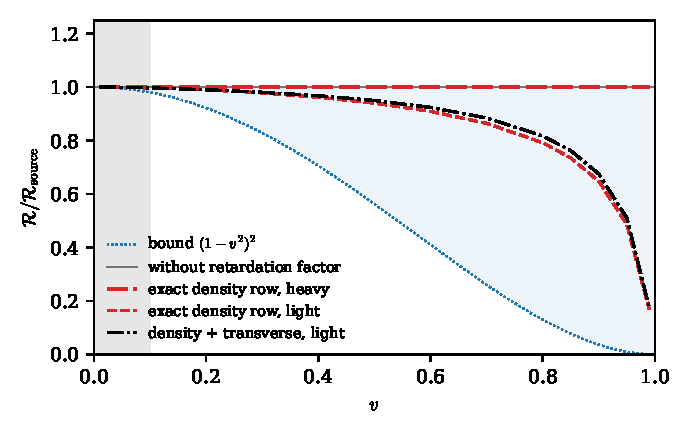
\includegraphics[width=0.82\linewidth]{figures/ch10/limit10_9b.pdf}
  \caption{Electron-recoil rate of silicon for dark matter of speed $v$, much heavier than the energy deposited, divided by the rate of the density row without the factor $(1 - \omega^2/\mathcal{Q}^2)^2$, against $v$. Red, long dashes: the exact density row \cref{eq:10.9-Drel} with a heavy mediator, which coincides with it to $10^{-4}$; red, short dashes: the same with a massless mediator; dash-dotted: the massless mediator with the transverse row of \cref{eq:10.9-fermi} added. Blue band: the range $[(1 - v^2)^2, 1]$ allowed by \cref{eq:10.9-bound}. Gray: $v \le 0.1$, where the bound guarantees agreement to \SI{2}{\percent}. Rates are integrated over $\omega$ from \SI{1.11}{eV}, the step-model gap that accompanies the tables, to \SI{89}{eV} and over $\mathcal{Q}$ from $\omega/v$ to \SI{22.5}{keV}. Loss function: random-phase with local fields, from the tables of \cref{sec:10.2}, held at its value at \SI{493}{eV} below that momentum. Transverse function: the measured $\varepsilon(\omega)$ of silicon at \SI{300}{K}~\cite{franta2017temperature}, with its Cherenkov pole integrated exactly; the transverse row counts the Cherenkov photons emitted above the gap as deposited energy, wherever they are absorbed.}
  \label{fig:10-boost-limit}
\end{figure}

\subsection{Fermionic absorption on electrons}\label{sec:10.9-fermionic}

A fermion $\chi$ of \SI{100}{keV} that is absorbed on an electron and leaves as a massless $\tilde\nu$ deposits $\omega = \mchi - q$ (\cref{eq:8.1-omega-ferm}). On a free electron at rest this is the recoil $q^2/2m_e$, so $q \simeq \mchi$ and $\omega \simeq \mchi^2/2m_e = \SI{9.8}{keV}$, a deposit that no halo particle of that mass could give by scattering. The momentum transfer is set by the rest energy and not by the speed of the dark matter, so that the rate is a single line through the response, independent of the halo. \Cref{sec:8.2-absorption} showed that the master formula holds with a sum over the momenta of $\tilde\nu$ and left the dark-matter tensor to be built here.

Take the operators $\Lambda_F^{-2}(\bar{\tilde\nu}P_L\chi)(\bar\psi\psi)$ and $\Lambda_F^{-2}(\bar{\tilde\nu}\gamma_\mu P_R\chi)(\bar\psi\gamma^\mu\psi)$ of \cref{sec:8.1-absorption}, with the chirality projectors $P_{L,R} = (1 \mp \gamma^5)/2$. Let $p = (\mchi, \vect{0})$ be the four-momentum of $\chi$ at rest and $k = (q, -\vect{q})$ that of $\tilde\nu$, so that $k\cdot p = \mchi q$. On the target side the scalar bilinear is the density row $n_e$ and the vector bilinear the current $J^\mu_e = (n_e, \vect{j}_e)$, up to terms of order $q/m_e$ (\cref{eq:C.15-bilinears}). On the dark-matter side, averaged over the spin of $\chi$ and summed over that of $\tilde\nu$, and with the trace identities of \cref{sec:10.9-boosted} together with $\Tr(\gamma^\mu\gamma^\nu\gamma^5) = 0$ and $P_L(\gamma\cdot p + \mchi)P_R = (\gamma\cdot p)P_R$,
\begin{gather*}
  \frac12\Tr\bigl[(\gamma\cdot k)P_L(\gamma\cdot p + \mchi)P_R\bigr] = k\cdot p = \mchi q , \\
  \frac12\Tr\bigl[(\gamma\cdot k)\gamma^\mu(\gamma\cdot p)\gamma^\nu P_L\bigr] = k^\mu p^\nu + k^\nu p^\mu - g^{\mu\nu}k\cdot p + \ii\epsilon^{\mu\nu\alpha\beta}k_\alpha p_\beta ,
\end{gather*}
up to the sign convention of the antisymmetric term. That term pairs with an antisymmetric current response, which a target with inversion symmetry and without magnetic order does not have, and we drop it. The relativistic normalization of the two dark-sector states divides by $2\mchi\cdot2q$. For the scalar operator the tensor is the number $\mathfrak{D}_{nn} = 1/4\Lambda_F^4$. For the vector operator, $\mathfrak{D}^{00} = 1/4\Lambda_F^4$, $\mathfrak{D}^{0i} = -q^i/(4q\Lambda_F^4)$ and $\mathfrak{D}^{ij} = \delta^{ij}/4\Lambda_F^4$, contracted with the responses of $J_\mu = (n_e, -\vect{j}_e)$. Continuity, $\hat{\vect{q}}\cdot\vect{j}_e \to (\omega/q)n_e$, turns the longitudinal current into the density, and the density, cross and longitudinal terms add to $(1 + \omega/q)^2S_{nn} = (\mchi/q)^2S_{nn}$. The transverse current, two components, keeps the weight one. With $\dd^3q/(2\pi)^3 = q^2\dd\omega/2\pi^2$ along the line $q = \mchi - \omega$, and with $\sigma_F = \mchi^2/4\pi\Lambda_F^4$,
\begin{keyresult}[Fermionic absorption on electrons]
\begin{equation}
  \begin{gathered}
  \frac{\dd\varGamma_S}{\dd\omega} = \frac{\sigma_F}{2\pi}\,\frac{q^2}{\mchi^2}\,\bar S_{nn}(q,\omega) , \\
  \frac{\dd\varGamma_V}{\dd\omega} = \frac{\sigma_F}{2\pi}\Bigl[\bar S_{nn}(q,\omega) + \frac{q^2}{\mchi^2}\,\Tr\bar S_{\vect{j}_{\mathrm{T}}\vect{j}_{\mathrm{T}}}(q,\omega)\Bigr] , \qquad q = \mchi - \omega ,
  \end{gathered}
  \label{eq:10.9-ferm}
\end{equation}
for the scalar and vector operators, at $v \to 0$ and for a massless $\tilde\nu$; the event rate per unit mass is $(\rho_\chi/\mchi\rho_T)\varGamma$, independent of the velocity distribution.
\end{keyresult}
\noindent For free electrons at rest, $\bar S_{nn} = 2\pi\nd_e\delta(\omega - q^2/2m_e)$ and the transverse current vanishes, and both rates are $\nd_e\sigma_F$ up to corrections of relative order $\mchi/m_e$, from the recoil of the electron~\cite[Eqs.~(1), (2) and (10)]{dror2021absorption}.

For an atomic shell the density response is the ionization form factor of \cref{eq:2.2-fion}: with the binding energy $E_B$ and the ejected energy $E_{\mathrm{ej}} = \omega - E_B$, the response per atom is $\pi|f_{\mathrm{ion}}(p_{\mathrm{ej}},q)|^2/2E_{\mathrm{ej}}$, both spins counted in $|f_{\mathrm{ion}}|^2$ as in Ref.~\cite[Eqs.~(A.18)--(A.21)]{essig2016direct}. The scalar rate of \cref{eq:10.9-ferm} then becomes $\dd\langle\sigma v\rangle_S/\dd E_{\mathrm{ej}} = \sigma_Fq^2|f_{\mathrm{ion}}|^2/(4E_{\mathrm{ej}}\mchi^2)$.

A light mediator changes the rate in a way that the dark-matter speed does not control. For the scalar operator mediated by a scalar of mass $m_{\mathrm{med}}$ with Yukawa couplings $y_{ee}$ and $y_{\chi\tilde\nu}$, $\Lambda_F^{-2}$ becomes $y_{ee}y_{\chi\tilde\nu}/(m_{\mathrm{med}}^2 - t)$, with $t$ the squared four-momentum transfer. On the $\tilde\nu$ leg, $t = (p - k)^2 = \omega^2 - q^2 = 2\mchi\omega - \mchi^2$, fixed by the rest energy, unlike the $-q^2$ of scattering. The rate is then the contact rate times $[m_{\mathrm{med}}^2/(m_{\mathrm{med}}^2 + \mchi^2 - 2\mchi\omega)]^2 = 1 - 2(\mchi^2 - 2\mchi\omega)/m_{\mathrm{med}}^2 + \dots$, the correction of relative order $(\mchi/m_{\mathrm{med}})^2$ that Cox, Dolan and Wood attach to the contact limit~\cite[Eqs.~(1), (2), (14) and (15)]{cox2024absorption}. It also tilts the spectrum, raising the high-$\omega$ end.

The two halves of this section meet when $\tilde\nu$ is massive. With $m_{\tilde\nu} = \mchi + \Delta_\chi$ and $|\Delta_\chi| \ll \mchi$, the outgoing fermion is slow, and \cref{eq:8.1-omega-inel} gives $\omega$ exactly as for inelastic scattering, with the recoil term computed with $\mchi$ instead of $m_{\tilde\nu}$ and the tensor multiplied by $\mchi/m_{\tilde\nu}$, both corrections of relative order $\Delta_\chi/\mchi$ (\cref{app:D.24}). Absorption into a nearly degenerate fermion is exothermic or endothermic scattering, and \cref{eq:10.9-inel} applies.

In practice the responses on the line $\omega = \mchi - q$ reach far above the valence scale. For $\mchi$ from the gap to \SI{1}{MeV} the momentum transfer runs into the cores of the atoms. The density row and the transverse current row are then needed from all-electron states, with Dirac--Hartree--Fock orbitals where $q \gtrsim m_e/3$.

\subsection{In-medium decay of an excited state}\label{sec:10.9-decay}

An excited state $\chi_2$ that survives from the early universe, or that a scattering in the Earth produces, can decay to $\chi_1$ inside the detector without touching anything, emitting a photon of energy $|\Delta_\chi|$. A transition magnetic moment $\mu_{\mathrm{M}}$ between the two states, $H = -\mu_{\mathrm{M}}\boldsymbol{\sigma}\cdot\vect{B}$ with $\boldsymbol{\sigma}$ the Pauli matrices between the spin states of $\chi_2$ and $\chi_1$, gives the vacuum rate
\begin{equation}
  \varGamma_{\mathrm{vac}} = \frac{\mu_{\mathrm{M}}^2|\Delta_\chi|^3}{\pi} ,
  \label{eq:10.9-vac}
\end{equation}
for $|\Delta_\chi| \ll \mchi$. This is the electric-dipole rate $\omega^3|\vect{d}|^2/3\pi$ of Heaviside--Lorentz units, with $|\vect{d}|^2$ replaced by the spin sum $\mu_{\mathrm{M}}^2\sum_f|\langle f|\boldsymbol{\sigma}|i\rangle|^2 = 3\mu_{\mathrm{M}}^2$. Baryakhtar and collaborators estimate the lifetime for a dipole operator $\bar\chi_2\sigma^{\mu\nu}\chi_1F_{\mu\nu}$ with coefficient $1/\Lambda_d$ as $\tau^{-1} \sim \pi|\Delta_\chi|^3/\Lambda_d^2$~\cite[Eqs.~(2.1) and (2.2)]{baryakhtar2020electromagnetic}. In the non-relativistic limit $\sigma^{\mu\nu}F_{\mu\nu} \to -2\boldsymbol{\sigma}\cdot\vect{B}$, so that $\mu_{\mathrm{M}} \simeq 2/\Lambda_d$, and \cref{eq:10.9-vac} gives $4|\Delta_\chi|^3/\pi\Lambda_d^2$, the same scaling. No operator of the target appears in the amplitude, and the master formula does not apply as it stands. The medium enters through the photon.

The decay rate follows from the golden rule with the magnetic field of the medium as the final state. At $T = 0$ the spectral density of the field is twice the imaginary part of its propagator, and in a medium the transverse propagator is $1/(\mathcal{Q}^2 - \omega^2\varepsilon^{\mathrm{T}})$, with $\vect{B} = \ii\vect{q}\times\vect{A}$. The spin average gives $\frac12\Tr(\sigma^i\sigma^j) = \delta^{ij}$, the transverse projection of $\vect{q}\times\vect{A}$ gives $2\mathcal{Q}^2$, and with $\omega = |\Delta_\chi|$, neglecting the recoil of $\chi_1$,
\begin{equation}
  \varGamma = \frac{2\mu_{\mathrm{M}}^2}{\pi^2}\int_0^\infty\dd\mathcal{Q}\;\mathcal{Q}^4\,\Imag\frac{1}{\mathcal{Q}^2 - \omega^2\varepsilon^{\mathrm{T}}(\mathcal{Q},\omega)} .
  \label{eq:10.9-decay}
\end{equation}
In vacuum $\Imag[1/(\mathcal{Q}^2 - \omega^2 - \ii0)] = \pi\delta(\mathcal{Q}^2 - \omega^2)$, and \cref{eq:10.9-decay} returns \cref{eq:10.9-vac}. In a transparent medium, $\varepsilon_2 \to 0$, the delta function sits at $\mathcal{Q} = \omega n_r$ with the refractive index $n_r = \sqrt{\varepsilon}$, and the rate is $n_r^3\varGamma_{\mathrm{vac}}$. The same calculation with the electric field, $\vect{E} = \ii\omega\vect{A}$, gives $n_r\varGamma_{\mathrm{vac}}$ for an electric dipole, local-field factors aside. The difference has a simple reason: the density of photon states grows as $n_r^2$ times the group index $n_{\mathrm{grp}}$, the electric field per photon falls as $1/(n_rn_{\mathrm{grp}})$, and the magnetic field per photon is $n_r$ times the electric one.

Where the medium absorbs, \cref{eq:10.9-decay} changes character. At large $\mathcal{Q}$ the integrand tends to $\omega^2\varepsilon_2^{\mathrm{T}}$, and the integral grows with the momentum up to which $\varepsilon_2^{\mathrm{T}}(\mathcal{Q},\omega)$ stays finite. That large-momentum part is not a photon. It is energy handed directly to the electrons near the particle through a virtual photon, a scattering $\chi_2 + \text{target} \to \chi_1 + \text{excitation}$. Its rate is the master formula with $\Delta_\chi < 0$, the magnetic-dipole operators of \cref{sec:8.1} and the transverse current row: the exothermic process of \cref{sec:10.9-inelastic} with a different vertex. The decay thus splits at an interface. The radiative part, a photon of energy $|\Delta_\chi|$ that is absorbed later or escapes, lies outside the response picture and is listed among the processes outside the framework in \cref{sec:22.3}. The non-radiative part lies inside it and needs $\varepsilon^{\mathrm{T}}$, or the transverse current response, at finite $\mathcal{Q}$.

Silicon shows the three regimes. Below the gap it is transparent, with $n_r = 3.44$ at \SI{0.5}{eV} and 3.54 at \SI{1.1}{eV}, and an excited state with a splitting there decays $n_r^3 = 41$ to 44 times faster inside the crystal than in vacuum, into a photon that the crystal does not absorb. Between 3.2 and \SI{22.5}{eV}, where $\Imag n_r > 0.1\Real n_r$, the decay is non-radiative, and its rate is the master-formula rate. Above the plasma frequency $n_r$ approaches one, from below as $1 - \omega_p^2/2\omega^2$ for a free electron gas and with small excursions at the $2p$ edge, and the vacuum rate holds within \SI{10}{\percent} for every splitting above \SI{55}{eV}.

\begin{limitbox}[In-medium decay of an excited state][lim:10.9d]
Vacuum decay through a transition dipole: $\tau^{-1} \sim \pi|\Delta_\chi|^3/\Lambda_d^2$ for the operator $(1/\Lambda_d)\bar\chi_2\sigma^{\mu\nu}\chi_1F_{\mu\nu}$~\cite[Eqs.~(2.1) and (2.2)]{baryakhtar2020electromagnetic}, in the book's form $\varGamma_{\mathrm{vac}} = \mu_{\mathrm{M}}^2|\Delta_\chi|^3/\pi$ (\cref{eq:10.9-vac}) with $\mu_{\mathrm{M}} \simeq 2/\Lambda_d$.
\par\smallskip
{\centering
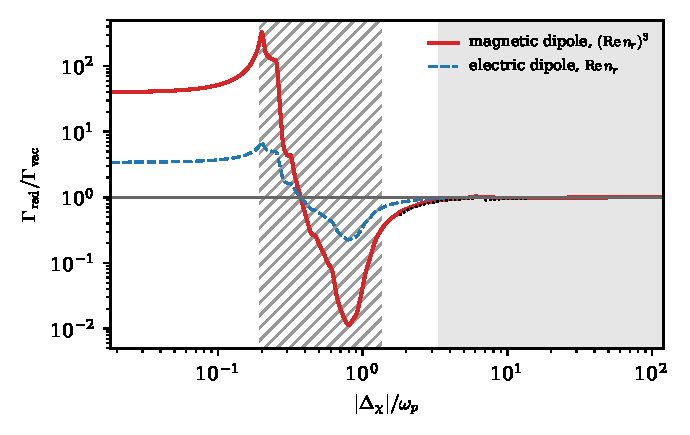
\includegraphics[width=0.82\linewidth]{figures/ch10/limit10_9d.pdf}
\captionof{figure}{Radiative decay rate of an excited state inside silicon over the vacuum rate, against the splitting $|\Delta_\chi|$ in units of the valence plasma frequency $\omega_p^{\mathrm{val}} = \SI{16.6}{eV}$. Red: magnetic dipole, $(\Real n_r)^3$; blue dashed: electric dipole, $\Real n_r$, local-field factors omitted. $n_r = \sqrt{\varepsilon}$ from the measured dielectric function of silicon at \SI{300}{K} below \SI{40}{eV}~\cite{franta2017temperature} and from atomic scattering factors above~\cite{henke1993xray}. Dotted: the free-electron-gas asymptote $n_r^3 \simeq 1 - 3\omega_p^2/2\omega^2$, with $\omega_p^{\mathrm{val}}$ below the $2p$ edge and the all-electron \SI{31.1}{eV} above. Hatched: $\Imag n_r > 0.1\Real n_r$, 3.2 to \SI{22.5}{eV}, where the radiative factor loses its meaning and the decay is a non-radiative transfer given by \cref{eq:10.9-decay} at finite $\mathcal{Q}$. Gray: splittings above \SI{55}{eV}, $3.3\,\omega_p^{\mathrm{val}}$, where $(\Real n_r)^3$ is within \SI{10}{\percent} of one.}\label{fig:10-decay-limit}
\par}
\smallskip
Below about $3\omega_p^{\mathrm{val}}$ the vacuum rate fails inside a solid: it is enhanced by $n_r^3 \approx 40$ in the transparent window of silicon below the gap and replaced by non-radiative transfer to the electrons where the crystal absorbs.
\end{limitbox}

\noindent No response of the target enters the vacuum rate; the medium acts only through $\varepsilon^{\mathrm{T}}$ at $\mathcal{Q} = \omega n_r$, and in a transparent medium the leading correction is the local field at the particle, which the macroscopic $\varepsilon$ does not contain.

\section{Nuisance parameters of the electronic rate}\label{sec:10.10}

A dark-matter particle of \SI{3}{MeV} with a heavy mediator and $\sigmae = \SI{e-37}{cm^2}$ makes $5.2\times10^4$ electron--hole pairs per kilogram-year in silicon if the electrons are independent, $2.5\times10^4$ if they screen in the random-phase approximation, and $1.85\times10^4$ once local fields are included. All three numbers come from the same published tables, counted from the low-temperature gap of \SI{1.17}{eV}, and they differ only in the many-body approximation. The last one is the best computed so far, but it is not the rate. The electron--hole attraction raises it, the conduction bands above the edge are uncertain at the level of a tenth of an eV, and two published tabulations of the same independent-particle response disagree by a third at this mass. \Cref{sec:8.8} turned each truncation into a nuisance parameter $\vartheta_k$, with the computed or estimated step to the next order as its template.

\subsection{Many-body spread}\label{sec:10.10-manybody}

The hierarchy of approximations of \cref{sec:4.6} is not an expansion in a small parameter, and its steps do not shrink. At \SI{3}{MeV} with a heavy mediator, random-phase screening lowers the independent-particle rate by \SI{52}{\percent}, and local fields lower what remains by a further \SI{26}{\percent}; for a light mediator the steps are \SI{76}{\percent} and \SI{18}{\percent}. The ratio of the independent-particle rate to the screened rate with local fields is 2.8 for a heavy mediator and 5.1 for a light one, between the values 2.3 and 9 that \cref{sec:10.2} found at 10 and \SI{1}{MeV}. A spread of this kind is not an uncertainty of the best approximation. Once an approximation is computed it becomes the central value, and the nuisance that remains is the step after it (\cref{sec:8.8}). For silicon that step is the electron--hole attraction, the excitonic (vertex) correction of the Bethe--Salpeter equation, and no finite-momentum calculation of it exists for silicon (\cref{sec:10.5}).

Its size can be estimated from the model of \cref{fig:10-xq}. At $|\vect{q}| = \SI{0.91}{keV}$ the attraction raises the screened loss function by 27 to \SI{29}{\percent} from the onset to \SI{3.5}{eV}, by \SI{49}{\percent} at \SI{4}{eV}, and by about \SI{30}{\percent} above, where part of the rise is an artifact of four conduction bands. A particle of \SI{3}{MeV} deposits at most $\tfrac12\mchi v_{\mathrm{max}}^2 = \SI{10.5}{eV}$, and the mean energy of its spectrum is \SI{4.7}{eV}. We take $\delta_{\mathcal{X}} = +0.28$ over that window, an estimate from a model at one momentum transfer, with the coupling block of \cref{eq:10.5-coupling} adding about $\pm0.10$ to it. The template has a definite sign: at $\vartheta_{\mathcal{X}} = 1$ the rate rises. By the $f$-sum identity \cref{eq:8.8-fsum} a many-body template is a tilt. Inside the \SI{10.5}{eV} window it raises the spectrum nearly uniformly and so acts like a normalization; the weight it moves comes from energies above the window, which the particle cannot reach. The same template, read at \SI{10}{MeV}, reaches \SI{35}{eV} and samples part of the compensating loss, so one $\vartheta_{\mathcal{X}}$ changes the rates at 3 and \SI{10}{MeV} by different fractions. The attraction also adds new support. The bound lines below the pair continuum carry the weight of the free continuum within $8.0\,E_x^b = \SI{0.12}{eV}$ of the edge (\cref{sec:10.5-lines}), which in the tables holds $4\times10^{-4}$ of the heavy-mediator rate at \SI{3}{MeV} and $1.5\times10^{-3}$ of the light-mediator rate. The tables resolve energies to \SI{0.2}{eV}, so these shares are orders of magnitude, and they matter only for thresholds at the gap.

A second nuisance sits inside the approximation already computed. At momentum transfers of two to three times the shortest reciprocal-lattice vector the local fields lower the per-$q$ rate of the tables by 1.67 at \SI{8}{keV} and 1.83 at \SI{10}{keV} (\cref{sec:10.2-corrections}). That size rests on a spectrum that holds only \SI{17}{\percent} of the $f$-sum below \SI{89}{eV} at \SI{10}{keV}. The model of \cref{fig:10-fcrys-limit}, built from a local pseudopotential with no input in common with the tables but the crystal structure, gives the same suppression. At \SI{5}{eV} and between 2 and $2.8\,q_0$ it finds the screened structure factor with local fields at 0.54 to 0.61 of the independent-particle one, with the head screening already within \SI{10}{\percent} of one above $2.2\,q_0$. The tables at the same energy and momenta give 0.40 to 0.48, with the head screening at 0.77 to 0.97 of the independent-particle value. Two calculations that share neither potential nor basis therefore agree that local fields hold the response near half of its unscreened value there, to within a quarter of each other. Both, however, lack the core-region oscillations of the valence states and the high-energy tail of the spectrum, and an all-electron calculation with enough bands is needed to fix the size (\cref{app:E.2,app:E.6}). The template is the change of the rate if the suppression above $2q_0 = \SI{7.46}{keV}$ were absent, $\vartheta = 1$ restoring the random-phase value there. It is $+0.067$ at \SI{3}{MeV} for a heavy mediator, where only \SI{7.5}{\percent} of the rate comes from those momenta, $+0.009$ for a light one, and $+0.24$ at \SI{10}{MeV}, where they hold \SI{29}{\percent} of the rate.

A third source is not a truncation of the label but of the numerics. The crystal form factor of \cref{sec:10.1} and the independent-particle head of the tables of \cref{sec:10.2} are the same quantity in the same approximation, computed with different codes, pseudopotentials and grids. With the same halo, each from its own onset, they give $1.60\times10^5$ and $1.36\times10^5$ events per kilogram-year at \SI{10}{MeV} for a heavy mediator, a ratio of 1.18, and 1.29 for a light one. At \SI{3}{MeV} the ratio is 1.34 for a heavy mediator and 1.55 for a light one. The difference sits at small $q$, where the lighter particle collects its rate, and the $f$-sum rule locates it. Between $0.3\,q_0$ and $0.7\,q_0$ the first moment of the form-factor table is 1.1 to 1.2 times the valence value (\cref{sec:10.1}), and that of the independent-particle head of the tables is 0.93 at every such momentum, partly because those tables end at \SI{89}{eV}. Neither table conserves the $f$-sum at small $q$, and the two violations lie on either side of it. The spread is measured with independent particles, but the central value is screened, and screening is strongest exactly at the small $q$ where the tables disagree. There a normalization error of $\varepsilon_2$ is partly screened out: if $\varepsilon_2$ and, by Kramers--Kronig, $\varepsilon_1 - 1$ are too large by $1 + \delta$ where $\varepsilon_1 \gg 1$, then $L \simeq \varepsilon_2/\varepsilon_1^2$ moves by about $1/(1 + \delta)$, opposite in sign and no larger. The independent-particle ratio is therefore an upper bound on the spread of the screened rate, and we carry it as such. \Cref{sec:8.8} named this case: for a truncation that breaks the $f$-sum the violation measures the error, and the spread between the calculations is the nuisance until a converged calculation passes the test (\cref{app:E.7}).

The Bethe--Salpeter step carries one more pitfall, an evaluation error rather than a truncation. A Bethe--Salpeter calculation that keeps only the resonant poles has the right $\varepsilon_2$ and the wrong $\varepsilon_1$, and it overstates the loss function by 2.12 at \SI{1.39}{keV} and \SI{1.3}{eV}, falling to within \SI{15}{\percent} of one above \SI{6.7}{keV} (\cref{eq:10.5-res}). Both time orderings remove it. It is listed below because a rate that inherits it is wrong by a factor that no nuisance of the correct calculation covers.

\subsection{Gap and threshold nuisances}\label{sec:10.10-gap}

The tables carry a scissor shift that places the conduction bands at the measured gap of silicon at zero temperature, \SI{1.17}{eV}~\cite[Sect.~III\,B]{knapen2021dark}, the gap a detector at millikelvin temperatures has, with the zero-point renormalization included in the measurement (\cref{sec:3.4}). The rate is counted from that gap, and the threshold mass is $m_{\mathrm{min}} = 2\Eg/v_{\mathrm{max}}^2 = \SI{0.333}{MeV}$. The \SI{1.11}{eV} that often accompanies these tables in analysis codes is a different number, the gap of the step model of pair creation with \SI{3.6}{eV} per pair (\cref{sec:1.5}), not the gap of the response. The energy nodes of the tables lie \SI{0.2}{eV} apart and do not resolve the edge itself.

What remains depends on what is measured. The edge itself is known to a few meV, and a shift of \SI{5}{meV} changes the \SI{3}{MeV} rate by \SI{0.4}{\percent}. A scissor, however, moves every conduction band by the same amount, and quasiparticle corrections in silicon differ from state to state by about \SI{0.1}{eV} (\cref{sec:3.4}). The bands above the edge are therefore uncertain at that level even when the edge is not. A shift of the whole spectrum by \SI{0.1}{eV} bounds this effect from above: it changes the \SI{3}{MeV} rate by $-7.5$ and $+8.0$ percent for a heavy mediator, by $\mp10$ percent for a light one, and the \SI{10}{MeV} heavy-mediator rate by \SI{4}{\percent}. The effect grows toward the threshold mass, where the spectrum samples only the first eV above the edge. For a target whose gap has not been measured the edge itself carries the \SI{0.1}{eV}, and $\delta\ln m_{\mathrm{min}} = \delta\ln\Eg$ turns it into \SI{8.5}{\percent} in the threshold mass of silicon (\cref{we:3-mmin-gap}). Near that mass the halo supply changes by orders of magnitude over a factor of two in $\mchi$, and the rate there depends on the gap more than on any other entry of the table below. The exciton binding of \SI{14.7}{meV} is a threshold nuisance of the same kind, which lowers the first line to \SI{1.155}{eV} (\cref{we:10-xline}), and \cref{tab:8-nuisances} carries it.

\subsection{Nuisance table of the electronic sector}\label{sec:10.10-table}

\Cref{tab:10-nuisances} lists the nuisances of the electronic sector. A next order computed in a model gives a template whose sign and shape are known and whose value may change once the real calculation is done. An estimate from a small parameter gives the size to a factor of order one. A spread between published calculations at the same order stands in for a template where the error lies outside the truncation label. An inequality gives a range without a central value, and for some items only the omission can be named.
\begin{table}[tbp]
  \caption{Electronic nuisances. Type in the classes of \cref{sec:8.8}: normalization, tilt (in $\omega$ or in $q$), threshold, new support, and class mix (weight moved between the zero-phonon and phonon-dressed sectors without changing the total). Basis of the size: ``model'' (next order computed in a model), ``tables'' (evaluated from the published tables), ``est.''\ (small-parameter estimate), ``spread'' (published calculations at the same order), ``bound'' (only an inequality is known), ``named'' (no size). Sizes are for silicon unless germanium is named, with rates at \SI{3}{MeV} for a heavy mediator. The last column gives the section where the open calculation is stated.}
  \label{tab:10-nuisances}
  \centering\small\setlength{\tabcolsep}{3pt}
  \begin{tabular}{@{}>{\raggedright\arraybackslash}p{0.26\linewidth}>{\raggedright\arraybackslash}p{0.13\linewidth}>{\raggedright\arraybackslash}p{0.34\linewidth}>{\raggedright\arraybackslash}p{0.09\linewidth}>{\raggedright\arraybackslash}p{0.12\linewidth}@{}}
    \toprule
    Truncation & Type & Size & Basis & Section \\
    \midrule
    Electron--hole attraction ($\mathcal{X}$: RPA + LF $\to$ BSE) & tilt; new support & $L$ up by 27--\SI{29}{\percent} near the edge at \SI{0.91}{keV}; rate $\delta_{\mathcal{X}} \approx +0.28$; lines $4\times10^{-4}$ of the rate & model & \cref{sec:10.5} \\
    Coupling block dropped (BSE in Tamm--Dancoff form) & tilt & about \SI{10}{\percent} of the proper $\varepsilon_2$ & est. & \cref{sec:10.5} \\
    Resonant-only real part (evaluation error) & tilt in $q$ & $L$ $\times2.12$ at \SI{1.39}{keV}, \SI{1.3}{eV}; within \SI{15}{\percent} above \SI{6.7}{keV} & tables & \cref{sec:10.5} \\
    Local fields at $q \gtrsim 2q_0$ (bands, pseudo-states) & tilt in $q$ & per-$q$ factor 1.67 (\SI{8}{keV}), 1.83 (\SI{10}{keV}); rate $+0.066$ if absent above $2q_0$ ($+0.24$ at \SI{10}{MeV}) & spread & \cref{sec:10.2} \\
    Independent-particle tabulation (code, grid, pseudopotential) & normali\-zation at small $q$ & IP rates differ by 1.34 (1.18 at \SI{10}{MeV}), an upper bound for the screened rate; $f$-sum 1.1--1.2 against 0.93 at $0.3$--$0.7\,q_0$ & spread & \cref{sec:10.1} \\
    Quasiparticle gap (rigid scissor) & threshold & edge measured, few meV; bands \SI{0.1}{eV}: rate $-7.5$/$+8.0\,\%$; $m_{\mathrm{min}}$ \SI{8.5}{\percent} without a measured gap & spread & \cref{sec:3.4} \\
    Plasmon decay into pairs with phonons ($n_g = 2$) & class mix & branching $10^{-3}$ to $10^{-2}$ & est. & \cref{sec:10.3} \\
    Local fields of the transverse current & normali\-zation & $-4$ to $-15\,\%$ (model); $-10$ to $-30\,\%$ (est.) & model & \cref{sec:10.4} \\
    Density--current cross term of a velocity coupling & normali\-zation & rate at least 16 (IP), about 29 (screened) times the static-electron formula at \SI{10}{MeV} & bound & \cref{sec:10.4} \\
    Triplet response beyond independent pairs & tilt & weight $\times2.2$ below \SI{3}{eV} (model); exchange splitting $\sim10^{-3}$ of the binding & model & \cref{sec:10.5} \\
    Final states of the germanium $3d$ shell & normali\-zation & $3d$/valence 0.07 (plane waves) against 0.69 (Fermi factor) at \SI{30}{MeV} & bound & \cref{sec:10.6} \\
    Screening of core transitions & normali\-zation & macroscopic \SI{2}{\percent} at \SI{12}{keV} (Ge); local fields not computed & est. & \cref{sec:10.6} \\
    Relativistic corrections (Pauli order) & normali\-zation & about $10^{-3}$, at most \SI{2}{\percent} (Ge $3d$); next order $3\times10^{-6}$ & est. & \cref{sec:10.6} \\
    Spin--orbit mixing at the germanium edge & tilt & up to \SI{10}{\percent} in amplitude & est. & \cref{sec:10.6} \\
    Terms of order $p_\phi^2$ in scalar absorption & new support near $\omega_p$ & density row equal to the kinetic rate at 16--\SI{18}{eV} (model) & named & \cref{sec:10.7} \\
    Room-temperature optical data near the edge ($n_T$) & threshold & more than $\times2$ within about \SI{20}{meV} of the edge & est. & \cref{sec:13.5} \\
    Bound shells in dark Compton scattering & tilt & K shell of Si at 45--\SI{100}{keV}, of Ge up to \SI{118}{keV}; L shells below \SI{20}{keV} & named & \cref{sec:10.8} \\
    Axial pair absorption with spin--orbit coupling & new support & of order $v^4$ without it & named & \cref{sec:10.8} \\
    Average over the directions of $\vect{q}$ & tilt in time & first anisotropic term $\ell = 4$ & named & \cref{sec:11.7} \\
    \bottomrule
  \end{tabular}
\end{table}

Two of these nuisances change the silicon rate at \SI{3}{MeV} by more than ten percent: the electron--hole attraction, by about a quarter, and the spread between tabulations of the independent-particle response, by a third for a heavy mediator and by half for a light one. At \SI{10}{MeV} the local fields at large momentum transfer join them, with a quarter, and the tabulation spread falls to a fifth. The gap stays below ten percent above \SI{3}{MeV} but grows without limit toward the threshold mass. Outside the density rows the largest items are not nuisances in the sense of a computed step. The cross term of a velocity coupling and the final states of the germanium $3d$ shell are known only between bounds, a factor of ten apart for germanium near \SI{30}{MeV}. A limit set on such a coupling has no central value yet, and the bound itself is what it can use (\cref{sec:10.4}).

One rule governs how the rows enter a likelihood. A truncation that two rates share acts on both with one $\vartheta_k$ (\cref{sec:8.8}). The attraction raises the rate at every mass and for both mediators at once, by different fractions, and a combination of masses or experiments that treated it as independent nuisances would let the data play one against the other. The inelastic, exothermic, boosted and fermionic rates of \cref{sec:10.9} read the same loss function and transverse current at shifted kinematics, and they carry the same nuisances with the same parameters; they add no rows of their own. Where one rate uses the tables and another the measured optical constants, as the scattering and absorption rates of \cref{sec:10.2,sec:10.7} do, the two share the many-body truncation only through what the measurement contains, and the absorption rate carries the temperature row instead.

\begin{workedexample}{The nuisance band on the silicon rate at \SI{3}{MeV}}\label{we:10-band3}
Take $\mchi = \SI{3}{MeV}$, a heavy mediator, $\sigmae = \SI{e-37}{cm^2}$ and the standard halo of \cref{sec:1.2}, with $\rho_\chi = \SI{0.3}{GeV.cm^{-3}}$. The kinematic window ends at $\omega = \SI{10.5}{eV}$ and $q = 2\mchi v_{\mathrm{max}} = \SI{15.9}{keV}$. The central value is the loss-function rate \cref{eq:10.2-rate} with the random-phase loss function with local fields of the tables of \cref{sec:10.2}, counted from the low-temperature gap of \SI{1.17}{eV}:
\begin{equation*}
  \mathcal{R}^{\mathfrak{T}} = \SI{1.85e4}{kg^{-1}.yr^{-1}} ,
\end{equation*}
about 51 events per kilogram and day. Its spectrum has a mean energy of \SI{4.7}{eV}, and \SI{10}{\percent} of it lies below \SI{3}{eV}.

Four nuisances act on this number with sizes in hand. In the power form \cref{eq:8.8-M}, $\mathcal{R}(\vartheta) = \mathcal{R}^{\mathfrak{T}}\prod_k(1 + \delta_k)^{\vartheta_k}$, each enters through $\ln(1 + \delta_k)$:
\begin{equation*}
  \begin{aligned}
  &\text{attraction, } \delta_{\mathcal{X}} = +0.28: & \ln(1 + \delta) &= +0.247, \\
  &\text{tabulation spread (bound), } +0.335: & &+0.289, \\
  &\text{band energies, } \SI{0.1}{eV}: & &-0.078, \\
  &\text{local fields above } 2q_0,\ +0.066: & &+0.064.
  \end{aligned}
\end{equation*}
The four are separate truncations with independent standard-normal $\vartheta_k$. To first order the logarithm of the rate then has the Gaussian width of \cref{eq:C.14-quadrature}, the four logarithms added in quadrature,
\begin{equation*}
  \sigma_{\ln\mathcal{R}} = \bigl(0.247^2 + 0.289^2 + 0.078^2 + 0.064^2\bigr)^{1/2} = 0.393 ,
\end{equation*}
and the rate lies between $\mathcal{R}^{\mathfrak{T}}/\ee^{0.393}$ and $\mathcal{R}^{\mathfrak{T}}\ee^{0.393}$ at one standard deviation:
\begin{equation*}
  \SI{1.25e4}{kg^{-1}.yr^{-1}} \le \mathcal{R} \le \SI{2.75e4}{kg^{-1}.yr^{-1}} ,
\end{equation*}
a factor of 1.48 either way. The attraction and the tabulation spread carry \SI{93}{\percent} of the variance. Taking the attraction at the upper value of the model, $+0.49$, widens the factor to 1.65; the coupling block, $\pm0.10$ on $\delta_{\mathcal{X}}$, changes $\ln(1 + \delta_{\mathcal{X}})$ by 0.075.

The band is not symmetric about the best guess. The attraction has a known sign, and $\vartheta_{\mathcal{X}} = 1$ moves the central value to $2.37\times10^4$; the band of the power form describes the uncertainty of where the next approximation lands, not a symmetric spread around the present one. The tabulation spread has no known sign, since the two tables miss the $f$-sum on opposite sides. For a light mediator the same steps give a central value of $6.0\times10^3$ and a factor of 1.67, with the tabulation spread at $+0.55$ and the gap at $-0.10$, and the local fields at large $q$ below one percent.

The band covers the truncations that the density response of silicon carries at this mass. It does not cover the halo, which the likelihood of \cref{eq:8.8-like} holds fixed, nor the detector, whose nuisances \cref{sec:21.4} adds. It is also wider than the step between the two best computed approximations, $2.49\times10^4$ to $1.85\times10^4$. That step is not an uncertainty, since it has been taken; the band covers the next step and the spread between calculations in the same approximation.
\end{workedexample}

\subsection{Open problems}\label{sec:10.10-open}

A finite-momentum Bethe--Salpeter calculation for silicon and germanium, with the coupling block kept and the bound lines added from computed masses and vertices, fixes the attraction, the coupling block, the triplet channel and the spin--orbit mixing at the germanium edge (\cref{sec:10.5,sec:10.6}; \cref{app:E.15}). An all-electron random-phase calculation with local fields, with enough bands to hold the $f$-sum at \SI{10}{keV} and with the current and kinetic rows carried as external rows of the Dyson equation, fixes the local fields at large $q$, the screening of core transitions, the transverse-current fields, the in-medium ratio of velocity couplings and the order-$p_\phi^2$ terms of scalar absorption (\cref{sec:10.2,sec:10.4,sec:10.7}; \cref{app:E.6,app:E.16}). Until these rows are computed, \cref{eq:10.4-band} is all a limit on a velocity coupling can use. Crystal conduction states for the germanium $3d$ shell, and a four-component response for the bound on relativistic terms, settle the core rows (\cref{sec:10.6}). A second-order electron--phonon calculation at the plasma frequency, and shell Compton profiles, settle the plasmon branching and the bound-shell correction to dark Compton scattering (\cref{sec:10.3,sec:10.8}; \cref{app:E.26}). The spread between tabulations needs no new physics, only one converged calculation that passes the $f$-sum test at small $q$.

The quadratic response, two published rates and the self-trapped excitons of NaI are open items that are not nuisances of the rates computed here. The interference between a contact amplitude and a second-order one needs the quadratic response of the crystal, which no reduction to two-point functions supplies (\cref{sec:10.8-open}). The free-electron vertex of fermionic absorption on a bound shell underestimates the rate by at least $1/r$, and the density row of cosmic-ray-boosted dark matter without its retardation factor overstates the rate at relativistic speeds (\cref{sec:10.9-open}). And the self-trapped excitons of NaI, where the Wannier picture fails, are open in every quantity that the rate needs (\cref{sec:10.5}).

\section*{Summary}

An electron--hole pair in silicon costs at least the gap, and the rate of making pairs is a contraction of the master formula with the response of the electrons (\cref{sec:10.1}). For independent electrons the structure factor is a sum over valence--conduction pairs with plane-wave vertices at the unfolded momentum transfer, and its angle average, rescaled, is the crystal form factor on which most published limits rest. Its normalization is where tabulations go wrong, and the $f$-sum rule tests it. From the published silicon form factor a \SI{10}{MeV} particle with a heavy mediator and $\sigmae = \SI{e-37}{cm^2}$ gives $1.60\times10^5$ events per kilogram-year, \SI{27}{\percent} of them from $q > 2q_0$, where pseudo-wavefunctions lose accuracy. The excess of its $f$-sum at small $q$ is only partly explained by the scissor shift.

Screening enters through one function, the loss function, and the loss-function rate is exact for a coupling to the total charge and for a coupling to the electron density at clamped nuclei or above the phonon band (\cref{sec:10.2}). In the published silicon tables the \SI{10}{MeV} rate is $1.36\times10^5$ for independent particles (two independent-particle tabulations differ by \SI{18}{\percent}, \cref{sec:10.10-manybody}), $8.6\times10^4$ with random-phase screening and $5.9\times10^4$ with local fields. The independent-particle rate is too high by 2.3 for a heavy mediator and 3.7 for a light one, and at the large momentum transfers that carry the heavy-mediator rate the local fields, not the head screening, do most of the work. The $f$-sum and the static step bound the rate of any target, loosely for silicon at MeV masses. A mediator that couples to electrons alone breaks the bound on the static step once the lattice relaxes, through the acoustic peak of the electrons that follow the nuclei.

The electron gas at the valence density reproduces the silicon rate within a factor 1.5 between 4.2 and \SI{9.5}{eV}, and fails below the absorption peaks, where it has no gap, and at large energies, where bound electrons carry momenta the gas lacks (\cref{sec:10.3}). Its plasmon is the pole of the inverse dielectric function, but halo dark matter cannot reach it: the slowest plasmon needs a particle faster than \SI{2860}{km.s^{-1}}. A plasmon made otherwise decays into pairs, and into pairs with phonons with a branching estimated at $10^{-3}$ to $10^{-2}$.

Couplings to the electron spin and current need responses beyond the density (\cref{sec:10.4}). Continuity, spin rotation and the product of inversion and time reversal reduce them to twelve real functions per momentum and energy in silicon and germanium, in a singlet block, screened, and a triplet block, unscreened. A velocity coupling adds the transverse current to the density, and a formula that keeps only the dark matter's velocity underestimates its rate in silicon at \SI{10}{MeV} by at least a factor 16 for independent particles, and about 29 with the density row screened.

The electron--hole attraction moves weight toward the gap and adds bound lines below it (\cref{sec:10.5}). In silicon the $1s$ line lies at \SI{1.155}{eV}, below the low-temperature gap of \SI{1.17}{eV}. In a model at \SI{0.91}{keV} the attraction raises the screened loss function by 27 to \SI{29}{\percent} near the edge. An evaluation that drops the antiresonant poles overstates the loss function by a factor 2.12 at small momentum transfer, and dropping the coupling block costs about \SI{10}{\percent}. The triplet channel has the singlet's lines without its local fields or screening.

Core shells enter at large momentum transfer (\cref{sec:10.6}). The germanium $3d$ shell opens at \SI{11.3}{keV} and overtakes the valence at \SI{12.5}{keV}; whether it dominates a rate depends on its final states, and with crystal states it does so above about \SI{30}{MeV} at a one-pair threshold. A filled, flat shell responds as a sum of independent atoms, without interference with the valence. Relativistic corrections to the response are about $10^{-3}$ and at most \SI{2}{\percent} for the shells halo dark matter reaches, and they shift the $f$-sum by $-0.24$ and $-0.76$ percent in silicon and germanium.

Absorbed bosons sample the response at zero momentum (\cref{sec:10.7}). A dark photon is absorbed with the loss function at its mass, suppressed 761 times at \SI{3}{eV} in silicon and enhanced 20 times at the plasmon, \SI{16.4}{eV}. An axion-like particle couples to the spin current, whose response without spin--orbit coupling is three quarters of the current response and is not screened; in a static magnetic field it converts like a dark photon. A scalar couples to the kinetic energy of the electrons, and mixes with the photon only at order $p_\phi^2$ in crystals without a polar axis.

Two insertions of the dark field reach rates that one insertion forbids (\cref{sec:10.8}). The absorption of a particle and its antiparticle is single absorption at twice the mass, and the pseudoscalar pair is absorbed through the axioelectric row without velocity suppression. Dark Compton scattering is the main signal of a dark photon in silicon above \SI{55}{keV}; its seagull form is exact to \SI{1}{\percent} below \SI{165}{keV}, and the published axion-like rate is too large by $(m_\phi + 2m_e)/(m_\phi + m_e)$, 1.836 at \SI{100}{keV}.

Inelastic, exothermic, boosted and fermionic dark matter use the same responses at other kinematics (\cref{sec:10.9}). An endothermic splitting of \SI{1}{eV} raises the lightest mass that makes pairs to \SI{0.60}{MeV}, and an exothermic one turns the spectrum into a halo-independent shell. For boosted particles with a massless mediator the exact density row is 0.65 of the published one at $v = 0.9$, and above $v = \varepsilon_1^{-1/2}$ the transverse row adds Cherenkov emission. An excited state below the gap decays radiatively 41 to 44 times faster inside silicon than in vacuum.

Each approximation of the chapter is a nuisance with a size (\cref{sec:10.10}). At \SI{3}{MeV} with a heavy mediator the silicon rate at the low-temperature gap is $1.85\times10^4$ events per kilogram-year, uncertain by a factor of 1.48 at one standard deviation. The electron--hole attraction and the spread between published independent-particle tables dominate; the gap and the local fields at large $q$ add less than ten percent each. Outside the density rows, the cross term of velocity couplings and the final states of the germanium $3d$ shell are known only between bounds. Throughout the chapter the nuclei were held fixed. \Cref{chap:11} releases them, and the energy a light particle deposits goes into phonons.


\printbibliography[heading=subbibliography]
